\chapter{MULTI-FACETED EVALUATION}
\label{ch:eval}

\section{Introduction}
%\lipsum[1]
%\ttfamily\lipsum[1]

%\paragraph{Evaluation.} 
Unsupervised learning systems like Multimorph are inherently difficult to evaluate. 
%This is because, supervised learning, the correct answers--e.g., the correct
%categories for the input examples are basically unknown. They are not supplied to the learner, at any rate. 
%This is because an unsupervised learning system is not provided with explicit learning targets.
Arguably, the main advantage of unsupervised learning is that it can discover novel and potentially useful categories and associations \citep{parsons:2004}. 
On the other hand, it is very difficult to evaluate previously unknown 
categories according to precision and recall. % and other measures that rely ``answer keys." 
The previously unknown categories in this study were morphological 
categories that would perhaps embody Aronoff's notion of the morphome \citep{aronoff:1994}.  
However, we did not know the precise form these categories would take. 

%---recall from REF that we use the term morph to avoid suggesting equivalence with he were unknown because we had  units were not conventional morphemes 
%or morphosyntactic categories. 

%Instead, MCMM-generated clusters corresponded roughly to Aronoff's 
%\emph{morphomes} \citep{aronoff:1994}, 
%which can be described as 
%\emph{pre-morphosyntactic} units, i.e., units that have been assembled from 
%phonemes, but have not yet been assigned 
%a syntactic or semantic meaning. I use the term \emph{morph} to refer to such units in what follows, since it is a less loaded term than either
%either \emph{morpheme} or \emph{morphome}.
%\emph{morphome}, since MCMM-generated clusters may not correspond 
%precisely to morphomes in every case (see section REF). %~\ref{sec:targets}).

Thus, the evaluation itself presented an important research question, namely that 
of how to evaluate the output of an unsupervised morphological clustering algorithm, 
particularly one that considers only features of word-internal form, having no 
access to morphosyntactic features that exist outside of the word, e.g., person, gender, and 
number of surrounding words.

%Multimorph is an unsupervised machine learning system, which makes it 
%intrinsically difficult to evaluate, and thus no single 
%evaluation method is likely to be perfect. 

I thus devised a multi-faceted approach to evaluating Multimorph's output, one comprising both
a qualitative and a quantitative component. The quantitative component, moreover, 
was itself a \emph{dual-paradigm}
evaluation approach, as it consisted of complementary \emph{intrinsic} and \emph{extrinsic} methods. 
%and  thus devised a dual-paradigm method for evaluating Multimorph's output, i.e., an approach consisting of two complementary methods, %I would thus rather not rely on a single method.
%not only because is it an unsupervised learning system, which are notoriously challenging to evaluate,  it learns unconventional morphological units, namely morphs. Indeed, it would be very difficult to come up with a gold standard for the morphs because we do not know what the morphs are supposed to look like; i.e., the ``right answers" are not obvious at the outset. 
%In particular, I will use 
%one \emph{intrinsic} and one \emph{extrinsic}. 
%The evaluation also included a \emph{qualitative} component, which served to complement the quantitative 
%utput of the MCMM was evaluated \emph{qualitatively}. The  which is intended to complement the quantitative
% intrinsic an extrinsic methods. 
 We will discuss each of these components in what follows. For the sake of simplicity,
we will only be using examples from the transcribed, stress-marked data (TS),
 but the discussion is equally applicable to
the other two types of data.


\section{Qualitative Evaluation} \label{sec:qualitative}
The qualitative component of the evaluation consisted mainly in manually examining the clusters generated by Multimorph's MCMM generated. These clusters are words grouped together according to shared elements of form. These shared elements can be immediately apparent to the human eye, especially to the eye of a linguist, but even in such cases they can be lost in an automated evaluation. %shared elements of form are immediately obvious to the human eye, but they can easily become lost in automated  
The qualitative component was meant to catch relationships---subtle or obvious---that might elude the automated 
quantitative evaluation. 
%A qualitative componentmponent is advantageous is that the automaticl,kl quantative procedures may not catch everything. 
%Humans also have linguistic intuition, and since we are dealing with linguistic data, which can be very useful in interpreting a cluster. Since we are dealing with unsupervised learning, there is basically no telling what the clusters will come to represent. The qualitative component is meant to address this lack of predictability.

\section{Quantitative Evaluation}
\subsection{Intrinsic Evaluation}
\label{sec:intrinsic}
An \emph{intrinsic} evaluation regards a system as a stand-alone system whose output is an end unto itself. An intrinsic evaluation thus judges a system's output directly as opposed to indirectly via the performance of a downstream system. However, intrinsic evaluations still require some \emph{externally-generated} standard against which to measure a system's performance. Such a \emph{gold standard} generally consists of a set of ``correct answers'' that humans have had some part in creating.
This study's intrinsic evaluation component thus required a 
set of \emph{gold-standard classes} against which to evaluate 
Multimorph's clusterings\footnote{Note the use of the word \emph{class} 
instead of \emph{cluster} in the phrase \emph{set of gold-standard classes}. 
By convention, gold-standard clusters are not actually called clusters, but rather 
(gold-standard) \emph{classes}} and measure the precision 
and recall of Multimorph's clusterings. 

In supervised learning, the training process requires that each learning example 
(or data point) have a target label, i.e., the ``correct answer.'' The target labels 
later serve as the gold-standard labels during the evaluation of the trained model. 
In supervised learning, therefore, it is trivial to obtain a gold-standard 
for evaluation; if a model was trained at all, then the gold standard 
already exists. By contrast, in unsupervised learning, obtaining a gold-standard 
dataset can be much less straightforward. One problem, as mentioned above, 
is that unsupervised learning is by nature open-ended; it is 
supposed to result in the discovery of categories and relationships.  

Another problem---one more specific to Multimorph 
itself---is
Multimorph's form-centric learning domain. Multimorph learns morphs, 
which are autonomous morphological categories, as discussed in chapter~\ref{autonomous}. 
They mediate between phonology and morphosyntax, but are at the same time independent 
of both of these levels of structure. It is thus not always clear what the morphs are in a 
given data set. As intermediate, \emph{pre-}morphosyntactic units, morphs are void 
of---and thus unconstrained by---meaning. They can thus be whatever they 
need to be in order to bridge the gap between phonological units 
and meaning (i.e., syntax and semantics).  There are not many morphomic lexicons 
or corpora wherein autonomous morphological units are annotated. There are no 
such resources for Hebrew.

There was in fact no ideal choice for a gold-standard dataset for Multimorph, 
not at the present time, at any rate. One of motivations behind this 
thesis was the lack of knowledge about the autonomous morphologies 
of individual languages, along with the notion that unsupervised learning could contribute to the 
process of discovering autonomous morphological categories. On the other hand, the lack
of corpora annotated with autonomous morphological categories meant 
that gold-standard datasets were not going to be readily available. Hebrew, at any rate,
lacks such a corpus. 
I chose to include this intrinsic evaluation component largely as means 
to supplement and support the highly experimental extrinsic evaluation 
component (see section~\ref{sec:eval-extrinsic}).  It was an exercise in maximizing the utility of less-than-ideal 
data---data that was not entirely
suitable for the present study's purposes.

\begin{figure}[t]
\begin{mdframed}
\begin{tabbing}
\hspace{1in} \= \hspace{5.5in} \kill
\vdots \> \vdots \\
hes\a'{i}gu \> pos:v\&root:nsg\&ptn:hifil\&tense:past\&pers:3\&gen:unsp\&num:pl \\
hev\a'{a}nt \> pos:v\&root:byn\&ptn:hifil\&tense:past\&pers:2\&gen:fm\&num:sg \\
hev\a'{a}nti \> pos:v\&root:byn\&ptn:hifil\&tense:past\&pers:1\&gen:unsp\&num:sg \\
hev\a'{e}\textipa{P}nu \> pos:v\&root:bw\textipa{P}\&ptn:hifil\&tense:past\&pers:1\&gen:unsp\&num:pl \\
hev\a'{e}\textipa{P}t \> pos:v\&root:bw\textipa{P}\&ptn:hifil\&tense:past\&pers:2\&gen:fm\&num:sg \\
hev\a'{e}\textipa{P}ta \> pos:v\&root:bw\textipa{P}\&ptn:hifil\&tense:past\&pers:2\&gen:ms\&num:sg \\
hev\a'{e}\textipa{P}tem \> pos:v\&root:bw\textipa{P}\&ptn:hifil\&tense:past\&pers:2\&gen:ms\&num:pl \\
hev\a'{e}\textipa{P}ti \> pos:v\&root:bw\textipa{P}\&ptn:hifil\&tense:past\&pers:1\&gen:unsp\&num:sg \\
hev\a'{i}n \> pos:v\&root:byn\&ptn:hifil\&tense:past\&pers:3\&gen:ms\&num:sg \\
hev\a'{i}na \> pos:v\&root:byn\&ptn:hifil\&tense:past\&pers:3\&gen:fm\&num:sg \\
\vdots \> \vdots \\
\end{tabbing}
\caption{Morphological analyses extracted from the Berman Longitudinal Corpus}
\label{fig:verb-analyses}
\end{mdframed}
\end{figure}

The source of Multimorph's input words was the 
Berman Longitudinal Corpus, as described in chapter~\ref{ch:experi}. Each word in this corpus is both (quasi-)phonetically 
transcribed as well as morphologically annotated, as described in chapter~\ref{ch:experi} 
(see in particular section~\ref{sec:morph-annotation}).
The first major step in 
building the gold-standard data was to extract each word's morphological analysis 
or analyses (section~\ref{sec:extr}). Figure~\ref{fig:verb-analyses} shows an excerpt from the full list
of analyses extracted from the corpus. The words in this excerpt happen to be verbs of the \textit{Hif`il}
\emph{binyan}. The lines of text in figure~\ref{fig:verb-analyses} are the 
beginnings of gold-standard morphological analyses, i.e., 
mappings from words to sets of gold-standard classes, with individual classes delimited by the 
\texttt{\&} symbol.  However, many of the BLC's categories are morphosyntactic and thus too abstract for our purposes, having little 
to do with actual form. I thus modified the BLC's categories, mapping them onto gold-standard classes that were
more form-based. We describe this mapping in section~\ref{sec:gld-std-classes}. 

The other major preliminary step in the intrinsic evaluation was to convert the MCMM's output, namely, the 
the $\mathbf{M}$ and $\mathbf{C}$ matrices, to an actual clustering of words. This was accomplished via
the process outlined in algorithm~\ref{alg:members}. The key principle governing this process was the following:
In order for a word to be counted as a member of a cluster, that cluster must be
responsible for at least one active reconstruction (or surface) unit in the word's reconstruction vector.
Clusters take responsibility for reconstruction units by ``voting'' for them. As described in chapter~\ref{ch:MCMM}, 
the votes of clusters
take the form $m_{i,k}c_{j,k}$, where $m_{i,k}$ is the activity of the $k$th hidden unit, that is, the $k$th cluster, and
$c_{j,k}$ is the weight between the $k$th hidden unit and the $j$th reconstruction unit.
%\textsc{Clusters-And-Members} algorithm\label{alg:members}
%The $\mathbf{M}$ and $\mathbf{C}$ matrices together provide all the information necessary 
%to derive a list of word-to-cluster mappings: The $\mathbf{M}$ 
%matrix tells us the indices of the clusters to which a given data point (or word) 
%belongs, and the $\mathbf{C}$ matrix provides a meaningful cluster label for each 
%cluster index. Each word-to-cluster mapping thus 
%consists of a word followed by a list of cluster labels.  
%as in ``runs: run, -s,"  where \textit{runs} is the word, and \textit{run} and \textit{-s} 
%are the labels of the clusters to which \textit{runs} belongs. These labels also represent 
%morphs. That is, e.g., \emph{-s} represents a cluster whose words end with the morph 
%\emph{-s}. 
%We will have more to say about gold-standard classes in section~\ref{sec:gld-std-classes}. 
\begin{algorithm}[t]
\DontPrintSemicolon % Some LaTeX compilers require you to use \dontprintsemicolon instead 
\KwIn{$\mathbf{M}$,  $\mathbf{C}$, input words $\mathbf{w}$, \text{threshold} $\theta$, $I$ $J$,$K$} 
\KwOut{$\mathbf{U}$, a list of \emph{clusters}, in which each cluster is a list of words. Let $\{\mathbf{u}_k$ denote the $k$th cluster, i.e., the list of \emph{words} that are the members of the $k$th cluster.}
Initialize cluster member lists: $\mathbf{U} = \{\mathbf{u}_0, \mathbf{u}_1, \mathbf{u}_2,\ldots, \mathbf{u}_K\}$ where each $\mathbf{u}_k \gets \emptyset$\;
\For {$ i \gets 0$ \textbf{to} $I$}{
	\For {$ k  \gets 0$ \textbf{to} $K$}{
	$j \gets 0$\;
		\While {$m_{i,k}c_{j,k} < \theta$ \textbf{and} $j < J$}{  \label{line:vote-thresh}
			$j \gets j + 1$\;
		}
	\If{$m_{i,k}c_{j,k} \geq \theta$}{
		$\mathbf{u}_k \gets \mathbf{u}_k \cup w_i$\; \label{line:append}
	}
	}
}
\Return $\mathbf{U}$\;
\caption{\textsc{Clusters-and-Members}}
\label{alg:members}
\end{algorithm}
% Recall also from chapter~\ref{ch:MCMM} that 
%% \emph{votes} 
%%% in an MCMM 
%% are products of the form $m_{i,k}c_{j,k}$, and that 
%the
As explained in chapter~\ref{ch:MCMM}, the 
 Noisy-OR mixing function requires at least one `\textsc{yes}' vote 
 in order to activate a given reconstruction unit.
 %, where votes are products 
 %of the form $m_{i,k}c_{j,k}$. 
 For Multimorph's 
 purposes, a vote is treated as a `\textsc{yes}' vote as long as it meets 
 %or exceeds the threshold $\theta_{\text{mc}}$.
 the criterion 
 \begin{equation}\label{eq:vote-criterion}
 m_{i,k}c_{j,k} \geq \theta_{\text{mc}}
 \end{equation}
 where $\theta_{\text{mc}}$ is the membership threshold. %In preliminary 
 In this study's experiments, $\theta_{\text{mc}}$ 
 was 
 set to 0.5.
 In algorithm~\ref{alg:members}, the \textsc{while}-loop condition on line~\ref{line:vote-thresh} enforces the threshold criterion. 
% ~\ref{line:vote-thresh}
%requires the current vote to be greater than (or equal to) to the membership threshold. 
 
 This \textsc{while} loop always begins with a particular $k$ index (that is, the index of the current cluster), which is supplied 
 by the loop within which the \textsc{while} loop is nested.
 The \textsc{while} loop proceeds to increment the index $j$ and thereby descend the cells of the ($k$th) 
 column in $\mathbf{C}$, that is,  $\mathbf{c}_k$, the current cluster's centroid vector. 
 Each  $j$ corresponds 
 to a different cell, i.e., a different  $c_{j,k}$, and thus a different vote 
 $m_{i,k}c_{j,k}$. 
The procedure visits each cell in turn until it finds a `\textsc{yes}' vote.
The Noisy-OR mixing function requires only one \textsc{yes} vote to verify that the data 
point (or word) in question is an active member of the $k$th cluster,
(see section~{\ref{sec:mixing-function}). The \textsc{while} loop thus terminates immediately upon finding 
 such a vote, whereupon
the current word is appended to the current cluster's list of active members (line~\ref{line:append}). 
This \textsc{while} loop is executed for each word in the input wordlist until the input words are exhausted, whereupon the procedure outputs a clustering in the form of a list of lists. Each inner list is a list of words and represents a cluster. 
 
If a vote $m_{i,k}c_{j,k}$ is greater than $0$ but \emph{less than} $\theta_{\text{mc}}$,
%for some $k$ and some feature $j$, 
we say that this vote indicates \emph{inactive} membership in the $k$th cluster; it is insufficient to
establish \emph{active} membership. If no \textsc{yes} vote exists for a data point, the data point is not an active member of 
%If data point is not an active member of any cluster,  be attributed to a cluster, that data point is not an active member
any cluster. We say that such a data point is not \emph{covered} by the clustering.  
%\threshold-exceeding vote for any $k \in K$ or $j \in J$---i.e., if \emph{none} of its features can be attributed
%to any cluster, then the data point is not an active member of any cluster, in which case, we say the data point (or word) is not \emph{covered} by the clustering. 
The concept of a clustering's \emph{coverage} will be relevant to our discussion of the results in chapter~\ref{ch:results}.
 
%In this way, the $\mathbf{M}$ and $\mathbf{C}$ matrices together provide all the information necessary 
%to derive a list of word-to-cluster mappings: The $\mathbf{M}$ 
%matrix tells us the indices of the clusters to which a given data point (or word) 
%belongs, and the $\mathbf{C}$ matrix provides a meaningful cluster label for each 
%cluster index. Each word-to-cluster mapping thus 
%consists of a word followed by a list of cluster labels.  
%as in ``runs: run, -s,"  where \textit{runs} is the word, and \textit{run} and \textit{-s} 
%are the labels of the clusters to which \textit{runs} belongs. These labels also represent 
%morphs. That is, e.g., \emph{-s} represents a cluster whose words end with the morph 
%\emph{-s}. 


\subsection{Gold-Standard Classes}
\label{sec:gld-std-classes}
As mentioned above, many of the BLC's categories are morphosyntactic in nature; for example, \emph{person}, \emph{number}, and \emph{gender} are independent categories in the BLC's morphological analyses. In Hebrew morphology, however, such categories are often not representative of autonomous morphological categories, i.e., categories based on form rather than syntax or semantics (see section~\ref{autonomous}). The problem in evaluating Multimorph, as mentioned above, is that Multimorph finds autonomous morphological categories rather than morphosyntactic ones. For this reason, I modified some of the BLC's categories to obtain gold-standard classes that were more directly tied to form. This section describes these modifications.  

\subsubsection{Verbs} 

 The Berman Longitudinal Corpus (BLC) uses the conventional conjugational categories for verbs exemplified in  
 tables~\ref{tab:hifil-paradigms} and \ref{tab:qal-paradigms}, 
  %tables~\ref{subtab:hifil-tensed} and \ref{subtab:hifil-part}, 
 which are essentially instances of Stump's \emph{content paradigm} \citep{stump:2001}. The content paradigm, as we discussed in section~\ref{sec:morpho-theories}, is to be distinguished from Stump's \emph{form paradigm}, since there is often a gap between these paradigms. We illustrated this gap in the case of the English present tense in table~\ref{tab:engverbpres}. As discussed in chapter~\ref{autonomous}, form-paradigm cells tend to be unnatural and thus morphomic. They are also therefore better suited than content cells to serve as form-based gold-standard classes. 

\begin{table}[!t] 
 %\label{tab:hifil-paradigms}
\centering
 %\footnotesize
 %\subtable[Tensed verb forms\label{subtab:hifil-tensed}]{
  \centering
 \setlength{\extrarowheight}{4pt}
 \begin{tabular}{lcccc}
 \toprule
 %\multicolumn{3}{c}{{\small \textit{Hif`il} Tensed Forms}} \\
    & \multicolumn{2}{c}{\small Past} & \multicolumn{2}{c}{\small Future} \\
    & \textsc{sg} & \textsc{pl} & \textsc{sg} & \textsc{pl} \\
\cmidrule{2-3}  \cmidrule{4-5}
   \textsc{1.m/f} & hi-tx\'{i}l-ti & hi-tx\'{i}l-nu & \textipa{P}e-tx\'{i}l & na-tx\'{i}l \\
   \hline
   \textsc{2.m} &  hi-tx\'{i}l-ta & hi-tx\'{i}l-tem  &  ta-tx\'{i}l & \\
  \textsc{2.f} & hi-tx\'{i}l-t & hi-tx\'{i}l-ten &  ta-txil-\'{i} & \raisebox{8pt}[0pt]{ta-txil-\'{u}}\\
   \hline
 \textsc{3.m} & hi-tx\'{i}l &   &  ya-tx\'{i}l & \\
 \textsc{3.f} & hi-txil-\'{a} & \raisebox{8pt}[0pt]{hi-txil-\'{u}} &  ta-tx\'{i}l & \raisebox{8pt}[0pt]{ya-txil-\'{u}} \\
   \bottomrule
 \end{tabular} \\\vspace{5pt}
 %} \\
  %\subtable[Participle forms\label{subtab:hifil-part}]{
  %\multicolumn{3}{c}{{\small \textit{Hif`il} Tensed Forms}} \\
 \centering
 \setlength{\extrarowheight}{4pt}
      \begin{tabular}{ccc}
      %\multicolumn{3}{c}{\textit{mzkir}  `he reminds'} \\
      %\toprule
      \multicolumn{3}{c}{{\small Participle (or Present)}} \\
       & \textsc{sg} & \textsc{pl} \\
      \midrule
      \textsc{m} & ma-tx\'{i}l & ma-txil-\'{i}m \\
      \textsc{f} & ma-txil-\'{a} & ma-txil-\'{o}t \\
      \bottomrule
      \end{tabular}
 %}
 \caption{Paradigms for the root \textit{t.x.l} in the \textit{Hif`il} binyan.}
 \label{tab:hifil-paradigms}
 \end{table}
 
 \begin{table}[!t]
 \vspace{12pt}
 \centering
 %\subtable[Tensed verb forms\label{subtab:qal-tensed}]{
 \centering
 \setlength{\extrarowheight}{4pt}
 \begin{tabular}{lcccc}
 \toprule
 %\multicolumn{3}{c}{{\small \textit{Qal} Tensed Forms}} \\
    & \multicolumn{2}{c}{\small Past} & \multicolumn{2}{c}{\small Future} \\
    & \textsc{sg} & \textsc{pl} & \textsc{sg} & \textsc{pl} \\
\cmidrule{2-3}  \cmidrule{4-5}
   \textsc{1.m/f} & gam\'{a}r-ti & gam\'{a}r-nu & \textipa{P}e-gm\'{o}r & ni-gm\'{o}r \\
   \hline
   \textsc{2.m} &  gam\'{a}r-ta & gam\'{a}r-tem  &  ti-gm\'{o}r & \\
  \textsc{2.f} & gam\'{a}r-t & gam\'{a}r-ten &  ti-gmer-\'{u} & \raisebox{8pt}[0pt]{ti-gmer-\'{u}}\\
   \hline
 \textsc{3.m} & gam\'{a}r &   &  yi-gm\'{o}r & \\
 \textsc{3.f} & gamr-\'{a} & \raisebox{8pt}[0pt]{gamr-\'{u}} &  ti-gm\'{o}r & \raisebox{8pt}[0pt]{yi-gmer-\'{u}} \\
   \bottomrule
 \end{tabular} \\\vspace{5pt}
 %}\\
 %\subtable[Participle forms\label{subtab:qal-part}]{
	 \centering
 	\setlength{\extrarowheight}{4pt}
      \begin{tabular}{ccc}
       %\toprule
     \multicolumn{3}{c}{\small Participle (or Present)}\\
       & \textsc{sg} & \textsc{pl} \\
      \midrule
      \textsc{m} & gom\'{e}r & gomr-\'{i}m \\
      \textsc{f} & gom\'{e}r-et & gomr-\'{o}t \\
      \bottomrule
      \end{tabular}
 %}
 \caption{Paradigms for the root \textit{g.m.r} in the \textit{Qal} binyan}
    \label{tab:qal-paradigms}
 \end{table}
I thus devised form-based gold-standard classes by grouping Hebrew verb inflections into form-based equivalence classes (essentially, form-paradigm cells). Table~\ref{tab:verb-cat-descriptions} summarizes the mappings from the BLC's conventional verb conjugational categories onto my form-based gold-standard classes. For example, the ``content" categories
\begin{center}
past-tense, 3rd-person plural \\
future-tense, 2rd-person masc plural \\
future-tense, 2rd-person fem plural \\
future-tense, 3rd-person plural \\
\end{center}
all map onto the single form-based class
\begin{center}
\texttt{(past\%3\%Pl)|(fut\%23\%Pl)}
\end{center}
where the \texttt{|} symbol means `or', and \texttt{\%} is a delimiter.

Note also the morphomic phenomena among the stems of the paradigms in tables~\ref{tab:hifil-paradigms} and \ref{tab:qal-paradigms}.
For instance, the future-tense forms in tables~ %\ref{subtab:hifil-tensed} and \ref{subtab:qal-tensed} 
\ref{tab:hifil-paradigms} and \ref{tab:qal-paradigms}.
have different stems from their past-tense counterparts. Following \citet{vance:2004}, we will refer to the future-tense stems as \emph{prefix stems} and the past-tense stems as \emph{suffix stems}. We do this for two main reasons: First, the prefix stems really do tend to take prefixes, while the suffix stems tend to take suffixes. Second, these stems are not always associated with past and future tenses, as participles take the prefix stem in some \emph{binyanim} (singular \emph{binyan}), e.g., the \textit{Hif`il} binyan; see the \textit{Hif`il} participles in table~\ref{tab:hifil-paradigms}. 
%thus added the gold-standard classes \texttt{prefix\_stem} and \texttt{suffix\_stem}, the former for future-tense stems, and the latter for past-tense stems. These classes are so named because in addition to their stem-internal differences, the ``prefix stems'' tend to take prefixes, while the ``suffix stems'' tend to suffixes (see \citet{vance:2004}). 
Moreover, the future stems in table~\ref{tab:hifil-paradigms} on the one hand differ from the future stems in table~\ref{tab:qal-paradigms} on the other. That is, 
%while there are prefix stems and suffix stems \emph{within} each of the two binyan paradigms.  
the prefix and suffix stems in table~\ref{tab:hifil-paradigms} differ as a group from those in table~\ref{tab:qal-paradigms} as group. The difference between paradigm-set~\ref{tab:hifil-paradigms} on the one hand and paradigm-set~\ref{tab:qal-paradigms} on the other is that these two groups are of different binyanim, namely the \emph{Hif`il} binyan and \emph{Qal} binyan, respectively.
 
 Thus, to fully specify a given verb stem, one needs to give both its \emph{binyan} and say whether it is a prefix or suffix stem. I thus added the \emph{derivational} gold-standard verb classes to complement the inflectional classes in table~\ref{tab:verb-cat-descriptions}. These follow the template
 \begin{equation}\label{eq:stem-temp}
\textit{binyan}  \, \texttt{\%} \, \{ \texttt{prefix\_stem}, \texttt{suffix\_stem} \}
 \end{equation}
 where \textit{binyan} can be any of the seven binyanim. For example, in the case of the \emph{Hif`il} verb \textit{hirb\'{a}cta}, this template would be filled in as 
  \begin{center}
    \texttt{hifil\&suffix\_stem}
  \end{center}
 A verb's full gold-standard instantiation for template~\eqref{eq:stem-temp} comprises its root, its stem type, and its inflectional class. Thus, for \textit{hirb\'{a}cta}, we have:
% is combined with the inflectional gold-standard class as well as the root as well 
% \textit{hirb\'{a}cta} is mapped onto gold-standard classes as follows:
\begin{center}
%\texttt{ pos:v\&root:rbc\&ptn:hifil\&tense:past\&pers:2\&gen:m\&num:sg} \newline
%\quad \mapsto \quad 
\texttt{root:rbc\&hifil\%suffix\_stem\&past\%2\%M\%Sg}
 \end{center}
 
 
\begin{table}[tb]
\centering
\subtable[One-to-one mappings from paradigm cells to categories\label{subtab:cats-one-to-one}]{
 \setlength{\extrarowheight}{6pt}
\begin{tabular}{lcl}
\toprule
Paradigm Cell &  & Gold-Standard Class \\
\midrule
past-tense, 1st-person singular & $\to$ & \texttt{past\%1\%Sg}\\ \hline
past-tense, 1st-person plural & $\to$ & \texttt{past\%1\%Pl}\\ \hline
past-tense, 2nd-person masc. singular & $\to$ & \texttt{past\%2\%M\%Sg} \\ \hline
past-tense, 2nd-person fem. singular & $\to$  & \texttt{past\%2\%F\%Sg} \\ \hline
past-tense, 3rd-person fem. singular & $\to$  & \texttt{past\%3\%F\%Sg} \\ \hline
future-tense, 1st-person singular & $\to$  & \texttt{fut\%1\%Sg} \\ \hline
future-tense, 1st-person plural & $\to$  & \texttt{fut\%1\%Pl}\\ 
\bottomrule
\end{tabular}
} \\
\subtable[Many-to-one mappings from paradigm cells to categories\label{subtab:cats-many-to-one}]{
 \setlength{\extrarowheight}{6pt}
\begin{tabular}{lcl}
\toprule
Paradigm Cells & &  Gold-Standard Class \\
\midrule
past-tense, 3rd-person plural & \multirow{4}{*}{$\to$} & \multirow{4}{*}{\texttt{(past\%3\%Pl)|(fut\%23\%Pl)}} \\
future-tense, 2rd-person masc plural & & \\
future-tense, 2rd-person fem plural & & \\
future-tense, 3rd-person plural & &\\
\hline
future-tense, 2rd-person masc. singular & \multirow{6}{*}{$\to$} & \multirow{6}{*}{\texttt{fut\%(2\%M)|(23\%F)}} \\
future-tense, 2rd-person masc plural &   & \\
future-tense, 2rd-person fem singular & &  \\
future-tense, 2rd-person fem plural & & \\
future-tense, 3rd-person fem singular & & \\
future-tense, 3rd-person fem plural & &\\
\bottomrule
\end{tabular}
}
%\label{tab:verb-cat-descriptions}
\caption{Mappings from conventional paradigm cells to form-based gold-standard classes} 
%and \ref{subtab:qal-tensed}) to gold-standard classes for Multimorph's intrinsic evaluation}
\label{tab:verb-cat-descriptions}
\end{table}
  
\subsubsection{Nominals}
\begin{description}
\item[Basic inflections.] Hebrew nominals, i.e., adjectives and nouns, 
inflect for gender and number. However, as discussed in chapter~\ref{autonomous}, 
particularly section~\ref{sec:heb-example}, the Hebrew inflectional endings 
for nominals are \emph{fusional}; it is impossible to separate the masculine plural suffix\textit{-im}, for instance, into 
distinct singular and plural components.
%\begin{figure}[t]
%\begin{mdframed}
%\begin{tabbing}
%\hspace{1in} \= \hspace{5.5in} \kill
%\vdots \> \vdots \\
%pas \> pos:n\&gen:ms\&num:sg\&stat:unsp\\
%pas\a'{e}y \> pos:n\&gen:ms\&num:pl\&stat:cstr pos:n\&gen:ms\&num:pl\&stat:bound\\
%pas\a'{i}m \> pos:n\&\&gen:ms\&num:pl\&stat:abs\\
%%qi\v{s}q\a'{u}\v{s} \> pos:n\&gen:ms\&num:sg\&stat:u\\
%%qi\v{s}u\textipa{P}\a'{i}m \> pos:n\&root:q\v{s}	extipa{P}\&ptn:CiCuC\&gen:ms\&num:pl\&stat:abs\\
%%qi\v{s}u\UTF{1E6D}\a'{i}m \> pos:n\&root:q\v{s}\UTF{1E6D}\&ptn:CiCuC\&gen:ms\&num:pl\&stat:abs\\
%%qi\v{s}\a'{u}\textipa{P} \> pos:n\&root:q\v{s}\textipa{P}\&ptn:CiCuC\&gen:ms\&num:sg\&stat:u\\
%%qi\v{s}\a'{u}\UTF{1E6D} \> pos:n\&root:q\v{s}\UTF{1E6D}\&ptn:CiCuC\&gen:ms\&num:sg\&stat:u\\
%qvuc\a'{a} \> pos:n\&root:qbc\&ptn:CCuCa\&gen:fm\&num:sg\&stat:unsp\\
%qvuc\a'{o}t \> pos:n\&root:qbc\&ptn:CCuCa\&gen:fm\&num:pl\&stat:bound \\
%zriq\a'{a} \> pos:n\&root:zrq\&ptn:CCiCa\&gen:fm\&num:sg\&stat:unsp \\
%zriq\a'{a}t	 \> pos:n\&root:zrq\&ptn:CCiCa\&gen:fm\&num:sg\&stat:bound \\
%%qlaf \> pos:n\&root:qlp\&ptn:CCaC\&gen:ms\&num:sg\&stat:u\\
%%qlaf\a'{i}m \> pos:n\&root:qlp\&ptn:CCaC\&gen:ms\&num:pl\&stat:abs\\
%%siman\a'{i}m \> pos:n\&root:sym\&ptn:CiCan\&gen:ms\&num:pl\&stat:abs\\
%%sim\a'{a}n \> pos:n\&root:sym\&ptn:CiCan\&gen:ms\&num:sg\&stat:u\\
%%sin\a'{a}r \> pos:n\&root:snr\&ptn:CiCaC\&gen:ms\&num:sg\&stat:u\\
%%sin\a'{o}r \> pos:n\&root:snr\&ptn:CiCoC\&gen:ms\&num:sg\&stat:u\\
%%sipr\a'{a} \> pos:v\&root:spr\&ptn:piel\&tense:past\&pers:3\&gen:fm\&num:sg\\
%%sipr\a'{u} \> pos:v\&root:spr\&ptn:piel\&tense:past\&pers:3\&gen:unsp\&num:pl\\
%%sipur\a'{e}y \> pos:n\&root:spr\&ptn:CiCuC\&gen:ms\&num:pl\&stat:cstr\\
%%sipur\a'{i}m \> pos:n\&root:spr\&ptn:CiCuC\&gen:ms\&num:pl\&stat:abs\\
%%sip\a'{a}rnu \> pos:v\&root:spr\&ptn:piel\&tense:past\&pers:1\&gen:unsp\&num:pl\\
%%sip\a'{a}rt \> pos:v\&root:spr\&ptn:piel\&tense:past\&pers:2\&gen:fm\&num:sg\\
%%sip\a'{a}rta \> pos:v\&root:spr\&ptn:piel\&tense:past\&pers:2\&gen:ms\&num:sg\\
%%sip\a'{a}rti \> pos:v\&root:spr\&ptn:piel\&tense:past\&pers:1\&gen:unsp\&num:sg\\
%%sip\a'{e}r \> pos:v\&root:spr\&ptn:piel\&tense:past\&pers:3\&gen:ms\&num:sg\\
%%wilon\a'{o}t \> pos:n\&root:wln\&ptn:CiCoCa\&gen:fem\&num:pl\&stat:u\\
%%wil\a'{o}n \> pos:n\&root:wyl\&ptn:CiCon\&gen:ms\&num:sg\&stat:u\\
%%tmun\a'{a} \> pos:n\&root:mnh\&ptn:CCuCa\&gen:fm\&num:sg\&stat:u\\
%%tmun\a'{o}t \> pos:n\&root:mnh\&ptn:CCuCa\&gen:fm\&num:pl\&stat:u\\
%\vdots \> \vdots \\
%\end{tabbing}
%\label{fig:blc-nouns}
%\caption{BLC morphological analyses for nouns}
%\end{mdframed}
%\end{figure}
   
   \begin{table}[t]
      \small
      \centering
       \setlength{\extrarowheight}{6pt}
      \begin{tabular}{ccc} 
 \toprule
 &  \textsc{sg} & \textsc{pl}\\
\cmidrule{2-3} 
\textsc{m} & pas & pas\'{i}m \\
\textsc{f}  &	qvuc\'{a}	& qvuc\'{o}t \\	
    \bottomrule
    \end{tabular}
    \caption{Fusional noun endings.}
    \label{tab:abs-only}
    \end{table}
 The same is true 
of the feminine plural suffix \textit{-ot}. (See section~\ref{sec:heb-example} for the full argument.)
We thus modify these atomic categories to make them match 
Hebrew's fusional suffixes. That is, we merged \texttt{masculine} 
and \texttt{plural} into the single category \texttt{m\%pl}. Likewise, 
\texttt{feminine} and \texttt{plural} became \texttt{f\%pl}, and \texttt{feminine} 
and \texttt{singular} became \texttt{f\%sg}.
We discard the part-of-speech category \emph{noun} because of its morphological vagueness; it corresponds to many different morphological exponents, but no \emph{particular} exponent.

\item[Construct State.]
The forms in table~\ref{tab:abs-only} are \emph{absolute} or \emph{free} forms. 
Nouns can also take \emph{construct} forms, i.e., the form used to create compound 
nouns and express genitive relationships. The construct state is characterized by 
certain changes in form with respect to the absolute forms. 
Examples~(\ref{ex:free-state}) and (\ref{ex:construct-phrase})
illustrate these changes.
In example~(\ref{ex:free-state}), the masculine plural form \textit{pas-\'{i}m} is an independent noun phrase 
and thus appears in the absolute state. In example~(\ref{ex:construct-phrase}), however, it is the head 
of a \emph{construct phrase} and thus takes the construct form \emph{pas-\'{e}y}. 
All of the four nominal inflectional categories are subject to stress loss and consequent 
vowel reduction/deletion, but only two of the four---the masculine plural and 
feminine singular---take distinctly construct suffixes, as shown in table~\ref{tab:cstr-endings}. 

\begin{exe}
\ex \textit{pas\'{i}m \quad weharaq\'{e}vet} \\ \label{ex:free-state} 
pas-\'{i}m \quad we-ha-raq\'{e}vet \\
stripe-\textsc{pl} \quad and-the-train \\
`stripes and the train'
\ex  \textit{pas\'{e}y \quad ha-raq\'{e}vet} \\ \label{ex:construct-phrase}
pas-\'{e}y \quad ha-raq\'{e}vet \\
stripe-\textsc{cstr.pl} \quad \textsc{def}-train \\
`the train tracks'
\end{exe}

   \begin{table}[t]
      \centering
      \setlength{\extrarowheight}{8pt}
         \small
      \begin{tabular}{ccccc} 
 \toprule
 &  \multicolumn{2}{c}{masculine} & \multicolumn{2}{c}{feminine} \\
 &  \textsc{sg} & \textsc{pl} & \textsc{sg} & \textsc{pl} \\
 \cmidrule{2-3} \cmidrule{4-5}
   \textsc{absolute} & pas & pas\'{i}m  & qvuc\'{a}	& qvuc\'{o}t \\
     \textsc{construct} & pas & pas\'{e}y & qvuc\'{a}t	& qvuc\'{o}t\\
    \bottomrule
    \end{tabular}
     \caption{Masculine and feminine construct forms}
             \label{tab:cstr-endings}
    \end{table}
    
%The formal difference between construct and absolute states is not always apparent 
In the other two categories, the masculine singular and feminine plural, 
the construct and absolute states are not always morphologically distinguished. 
Because these categories lack distinct construct suffixes, any formal distinction must 
be provided by vowel reduction/deletion. However, in Modern Hebrew, vowels are 
not uniformly subject to reduction and deletion, a consequence of the 
persistent influence of Biblical Hebrew prosody \citep{morag:1959, bolozky:1997, ravid-and-shlesinger:2001}. 
For instance, some vowels are protected from deletion because their 
Biblical Hebrew antecedents were intrinsically (and thus unchangeably) long. 
Other vowels are protected if they occur in a closed syllable.\footnote{Sometimes 
a vowel in an open syllable is protected because the syllable \emph{would have been} 
closed in Biblical Hebrew, which recognized geminate consonants as a sequence of two 
moras. For instance, the word \textit{tabbax} `cook, chef,' is pronounced [tabax] in Modern Hebrew---without the geminate /b/. Nevertheless, historical geminate \textit{b} protects the initial /a/ from deletion in the construct phrase [tabax  mi\v{s}k\'an] `resident chef' \citep[see][p. 43]{bolozky-and-schwarzwald:1990}.}

Thus, in the transcriptional data (both with and without stress marking), there 
is sometimes no formal marker (or exponent) of the construct state in the masculine singular 
and feminine plural categories. 
Moreover, in the orthographic data, there is \emph{never} a distinction between 
the absolute and construct states in these 
two categories, since the vowels that are subject to reduction/deletion are not represented in the 
orthographic data in the first place.
Therefore, when the BLC category \textit{stat:bound} (i.e., construct state) 
is associated with a masculine singular or feminine plural nominal, we discard it, 
as in examples~(\ref{ex:cstr:m-sg}) and (\ref{ex:cstr:f-pl}). Otherwise, we fuse 
it to the \textsc{gender}\%\textsc{number} categories as \textit{cstr}, as 
in examples~(\ref{ex:cstr:m-pl}) and (\ref{ex:cstr:f-sg}).

\begin{exe}
\ex  
\begin{xlist}
		\ex gen:ms\&num:sg \&stat:bound \quad $\to$ \quad \texttt{m\%sg} \label{ex:cstr:m-sg}
		\ex gen:ms\&num:pl\&stat:bound \quad $\to$ \quad \texttt{cstr\%m\%sg} \label{ex:cstr:m-pl}
		\ex gen:fm\&num:sg\&stat:bound  \quad $\to$ \quad \texttt{f\%pl} \label{ex:cstr:f-sg}
		\ex gen:fm\&num:pl\&stat:bound \quad $\to$ \quad \texttt{cstr\%f\%pl} \label{ex:cstr:f-pl}
	\end{xlist} \label{ex:cstr-cats}
\ex  
\begin{xlist}
		\ex pos:adj\&gen:ms\&num:sg \quad $\to$ \quad \texttt{adj\&m\%sg} \label{ex:adj:m-sg}
		\ex pos:adj\&gen:ms\&num:pl \quad $\to$ \quad \texttt{adj\&m\%pl} \label{ex:adj:m-pl}
		\ex pos:adj\&gen:fm\&num:sg \quad $\to$ \quad \texttt{adj\&f\%sg} \label{ex:adj:f-sg}
		\ex pos:adj\&gen:fm\&num:pl \quad $\to$ \quad \texttt{adj\&f\%pl} \label{ex:adj:f-pl}
	\end{xlist} \label{ex:adj-cats}
\end{exe}

\item[Adjectives.]
As discussed in chapter~\ref{autonomous} (section~\ref{sec:heb-example} in particular), 
a large number of Modern Hebrew adjectives are derived by attaching the 
suffix -\textit{i}
to a noun. Thus, unlike nouns, many adjectives have a formal exponent, i.e., a particular aspect of form that distinctly corresponds to the category \emph{adjective}---at least the adjectives derived via -\textit{i} do, anyway. 
We therefore retained
\texttt{pos:adj} (i.e., \textit{part-of-speech: adjective}) as a gold-standard class.
(Recall that we discarded the \emph{noun} category because it lacked particular formal exponent.) 
However, this treatment of adjectives is imperfect because many adjectives, such as
\textit{nexm\'{a}d} `pleasant' (see table~\ref{tab:non-y-adjs}),
lack a distinctive adjectival marker.  This is one of many ways in which the category mapping described in this section is an imperfect solution to the problem of obtaining suitable gold-standard classes.  
% he masculine-singular category is generally unmarked. However, masculine-singular adjectives derived via the \textit{-i} suffix, corresponds to masculine-singular infectional category; the other
%three categories bear the \textit{-i} suffix along with an additional ending. 
 
%\begin{figure}[t]
%\begin{mdframed}
%\begin{tabbing}
%\hspace{1in} \= \hspace{5.5in} \kill
%nexmad\a'{a} \> pos:adj\&root:xmd\&ptn:niCCaC\&gen:fm\&num:sg\&src:deverb\\
%nexmad\a'{i}m \> pos:adj\&root:xmd\&ptn:niCCaC\&gen:ms\&num:pl\&src:deverb\\
%nexmad\a'{o}t \> pos:adj\&root:xmd\&ptn:niCCaC\&gen:fm\&num:pl\&src:deverb\\
%nexm\a'{a}d \> pos:adj\&root:xmd\&ptn:niCCaC\&gen:ms\&num:sg\&src:deverb\\
%\end{tabbing}
%\label{fig:non-y-analyses}
%\caption{Morphological analyses extracted from the Berman Longitudinal Corpus. These entries are the inflections
%of the adjective \textit{nexmad} `pleasant.'}
%\end{mdframed}
%\end{figure}

   \begin{table}[t]
      \small
      \centering
       \setlength{\extrarowheight}{8pt}
      \begin{tabular}{ccc} 
 \toprule
 & \textsc{sg} & \textsc{pl} \\
\cmidrule{2-3}
    \textsc{m} & nexmad & nexmad-\'{i}m \\
   \textsc{f} &  nexmad-\'{i} & nexmad-\'{o}t \\
    \bottomrule
    \end{tabular}
    \caption{Inflections of the adjective \textit{nexmad} `pleasant'}
        \label{tab:non-y-adjs}
    \end{table}

%\begin{table}[ht]
%\begin{center}
%\subtable[maqomi `local' \label{subtab:fusion:1}]{
%\setlength{\extrarowheight}{8pt}
%{\begin{tabular}{lcc}
%\  & masc & fem  \\
%\hline 
%sg & maqom-i & meqom-i-t  \\
%pl & meqom-iy-im & meqom-iy-ot  \\
%\end{tabular}}
%}
%\subtable[gadol `big' \label{subtab:fusion:2}]{
%\setlength{\extrarowheight}{8pt}
%{\begin{tabular}{lcc}
%\  & masc & fem  \\
%\hline 
%sg & gadol & gdol-a  \\
%pl & gdol-im & gdol-ot  \\
%\end{tabular}}
%}
%\label{tab:fusion}
%\caption{Fusional suffixes in Hebrew nominals}
%\end{center}
%\end{table}

\begin{table}[bt]
\centering
\small
\setlength{\extrarowheight}{8pt}
\begin{tabular}{lcc}
\toprule
& \textsc{sg} & \textsc{pl}  \\
\cmidrule(lr){2-3}
\textsc{m} & maqom-\'{i} &  meqom-iy-\'{i}m\\
\textsc{f} & meqom-\'{i}-t  & meqom-iy-\'{o}t  \\
\bottomrule
\end{tabular}
\caption{Inflections of the adjective \textit{maqom\'{i}} `local,' derived from the noun for \textit{maqom} `place' via the suffix \textit{-i}/\textit{-y}}
\label{tab:der-adjs}
\end{table}

%\texttt{cstr\%f\%mass}
%\texttt{cstr\%f\%sg}
%\texttt{cstr\%m\%mass}
%\texttt{cstr\%m\%pl}
%\texttt{cstr\%m\%sg}
%\textit{state} \% \textit{gender} \% \textit{number}
%\textit{adj}\%\textit{m}\%\textit{sg}

%\begin{exe}
%\ex \label{ex:cstr:pasey}
%	\textsf{pas\'{e}y+ha+rak\textipa{\'{e}}vet} \\
%	\textsf{n:det|+n|pas\&gen:ms\&num:pl\&stat:comp-\'{e}y+det|ha+n|rak\textipa{\'{e}}vet}
%\ex \label{ex:cstr:shaat} 
%	\textsf{\v{s}\textglotstop{at}+sip\'{u}r .} \\
%	\textsf{n|+n|\v{s}a\textipa{Q}\'a\&gen:fm\&num:sg\&stat:comp-\'at+n|sip\'ur .}
%\ex \label{ex:cstr:bdiqat} 
%	\textsf{bdiq\'{a}t+\textipa{P}ozn\'{a}yim} \\ 
%	\textsf{n|bdiq\'{a}\&root:tbd\&ptn:tbd\&gen:fm\&num:sg\&stat:bound-\'{a}t}
%\end{exe}

%Therefore, when the BLC category \textit{stat:bound} is associated with a masculine singular or feminine plural nominal, we discard it, as in examples~{ex:cstr:m-sg} and {ex:cstr:f-pl}. Otherwise, we fuse it to the \textsc{gender}\%\textsc{number} categories as \textit{cstr}, as in examples~{ex:cstr:m-pl} and {ex:cstr:f-sg}.

\item[Participles.]
As in English, participles in Hebrew can function as nouns and adjectives.
All binyanim except the \textit{Qal} and \textit{Nif`al} use 
the prefix stem to form the participle. The \textit{Nif`al} uses the prefix stem, 
and the \textit{Qal} uses a different set of stems altogether to form the 
participle.\footnote{The participle functions as the present-tense verb form in modern Hebrew, but it inflects as a nominal category.}
For \textit{Qal} and \textit{Nif`al} participles, we add the categories \texttt{qal:participle} 
and \texttt{nifal:suffix\_stem}.  In general, the BLC category \texttt{pos:part} 
is combined with the fusional gender and number endings to categories like \texttt{part\%m\%sg}.

%def analysisFilter(analyses_str):
%	new_analyses = list()
%	analyses=analyses_str.split()
%	if "pos:part" in analyses_str:
%		####print "**",analyses_str
%		for analysis in analyses:
%			if "pos:v" in analysis:
%				continue
%			elif "pos:adj" in analysis:
%				continue
%			elif "pos:n" in analysis:
%				continue
%			else: new_analyses.append(analysis)
%		return new_analyses
%	else:
%		return analyses
%	elif pos == "part":
%		#pat = ur"(ptn:)([a-zC]+)(&tense:)(past)(&pers:3&gen:f&num:sg)(&|$)"
%		#pat = ur"(pos:)(part)(&[^\s]*)(&ptn:)([a-zC]*)(&[^\s]*)(&gen:)([mfu])(&num:)([sgplundoma]+)(&|$)"
%		#pat = ur"(pos:)(part)(&root:[^\s]+&ptn:)([a-zC]*)(&[^\s]*)(gen:)([mascfemunsp]+)(&num:)([sgplundoma]+)(&|$)"
%		pat = ur"(pos:)(part)([^\s]*&root:[^\s]+)(&ptn:)([a-zC]*)(&[^\s]*)(gen:)([mascfemunsp]+)(&num:)([sgplundoma]+)(&|$)"
%		re_part = re.compile(pat, re.UNICODE)
%		#analysis = re_part.sub(ur"\5%prefix_stem&\8%\10\11\6", analysis)
%		if ptn == "qal":
%			#1 (pos:)
%			#2 (part)
%			#3 ([^\s]*&ptn:)
%			#4 ([a-zC]*) the actual pattern
%			#5 (&[^\s]*)
%			#6 (gen:) 
%			#7 ([mascfemunsp]+)  # gender val
%			#8 (&num:)
%			#9 ([sgplundoma]+)    # number val
%			#10(&|$)
%			analysis = re_part.sub(ur"\3&\5%participle&\8%\10\6", analysis)
%			# stemFeature = binyan + "%participle"
%			# processedFeatures.append(stemFeature)
%		elif ptn == "nifal":
%			analysis = re_part.sub(ur"\3&\5%suffix_stem&\8%\10\6", analysis)
%			# stemFeature = binyan + "%suffix_stem"
%			# processedFeatures.append(stemFeature)
%		else:
%			analysis = re_part.sub(ur"\3&\5%prefix_stem&\8%\10\6", analysis)
			
\item[Free-standing pronouns] include the personal and demonstrative pronouns presented in 
tables~\ref{tab:pers-pronouns} and \ref{tab:dem-pronouns}, respectively.
Like verbs, personal pronouns have person, number, and gender, each of which is treated as 
an atomic morphosyntactic feature in the BLC analyses, as illustrated in 
table~\ref{tab:pers-pronouns}. For each personal-pronoun morphological analysis, 
we map the person, gender, and number categories onto
two gold-standard classes: one combining person and gender 
into a single class, e.g., \texttt{pro:pers\%2\%m} (2nd-person $\land$ masculine), 
and another combining person, gender, and number, 
e.g., \texttt{pro:pers\%2\%m\%sg} (2nd-person $\land$ masculine $\land$ singular). 
The former type of gold-standard class
thus corresponds to a particular row in table~\ref{tab:pers-pronouns}, 
while the latter corresponds to a particular \emph{cell} in this table.
\begin{table}[tb]
\centering
%[Personal pronouns\label{tab:pers-pronouns}]{
\setlength{\extrarowheight}{6pt}
\begin{tabular}{lcc}
\toprule
      & \textsc{sg} & \textsc{pl} \\
     \midrule
    \textsc{1.m/f} & \textipa{P}an\'{i} & $\{$ \textipa{P}an\'{a}xnu, \textipa{P}\'{a}nu $\}$ \\
    \midrule
 \textsc{2.m} &  \textipa{P}at\'{a}  &  \textipa{P}at\'{e}m\\
   %\textit{2.m}  & fem & \textipa{P}at  &  \textipa{P}at\'{e}n\\
  \textsc{2.f} & \textipa{P}at  &  \textipa{P}at\'{e}n\\
   \midrule
 \textsc{3.m} & hu\textipa{P} & hem\\    
   %\raisebox{1.5ex}[0pt]{3} & fem  & hi\textipa{P} &  hen \\
   \textsc{3.f} & hi\textipa{P} &  hen \\
    \bottomrule
\end{tabular}
\caption{Personal pronouns}
\label{tab:pers-pronouns}
\end{table}

\begin{table}[tb!]  
\setlength{\extrarowheight}{6pt}
\centering
\begin{tabular}{lcc}
\toprule
 & \textsc{sg} & \textsc{pl} \\
  \cmidrule{2-3}   
 \textsc{m} & ze & {\textglotstop}\'{e}le \\ 
   %\raisebox{1.5ex}[0pt]{3} & fem  & hi\textipa{P} &  hen \\
\textsc{f} & \{ zo, zo\textipa{P}t \}  &  {\textglotstop}\'{e}lu \\
   \bottomrule
  \end{tabular}
\caption{Demonstrative pronouns}
  \label{tab:dem-pronouns}
  \end{table}
  
%  \begin{exe}
%\ex \label{ex:pro-pers-2f}\begin{xlist}
%		\ex \texttt{pro:person\&pers:2\&gen:fm\&num:sg} \quad $\to$ \quad \texttt{pro:person\%2\%f\&pro:person\%2\%f\%sg}
%		\ex \texttt{pro:person\&pers:2\&gen:fm\&num:pl} \quad $\to$ \quad \texttt{pro:person\%2\%f\&pro:person\%2\%f\%pl}
%	\end{xlist}
%\ex \label{ex:pro-pers-2m} \begin{xlist}
%		\ex \texttt{pro:person\&pers:2\&gen:ms\&num:sg} \quad $\to$ \\ $\qquad \qquad$ \texttt{pro:person\%2\%m\&pro:person\%2\%m\%sg}
%		\ex \texttt{pro:person\&pers:2\&gen:ms\&num:pl} \quad $\to$ \\ {} $\qquad \qquad$ \texttt{pro:person\%2\%m\&pro:person\%2\%m\%pl}
%	\end{xlist}
%\end{exe}

%  \begin{figure}[t]
%  \begin{mdframed}
% \begin{tabbing}
%\hspace{1in} \= \hspace{5.5in} \kill
%\v{s}ehem \> pre:sh\&pre:sh\&pos:pro:person\&pers:3\&gen:ms\&num:pl \\
%\v{s}ehen \> pre:sh\&pre:sh\&pos:pro\_person\&pers:3\&gen:fm\&num:pl\\
%\v{s}e\textipa{P}an\a'{i} \> pre:sh\&pos:pro:person\&pers:1\&num:sg \\
%\v{s}e\textipa{P}at\a'{a} \> pre:sh\&pre:sh\&pos:pro\_person\&pers:2\&gen:ms\&num:sg\\
%\v{s}e\textipa{P}at\a'{e}m \> pre:sh\&pre:sh\&pos:pro\_person\&pers:2\&gen:ms\&num:pl\\
%\textipa{P}an\a'{a}xnu \> pos:pro:person\&pers:1\&num:pl\\
%\textipa{P}an\a'{i} \> pos:pro:person\&pers:1\&num:sg\\
%\textipa{P}at\a'{e}m \> pos:pro:person\&pers:2\&gen:ms\&num:pl\\
%\textipa{P}at\a'{e}n \> pos:pro:person\&pers:2\&gen:fm\&num:pl\\
%hu\textipa{P} \> pos:pro:person\&pers:3\&gen:ms\&num:sg \\
%hi\textipa{P} \> pos:pro:person\&pers:3\&gen:fm\&num:sg \\
%\end{tabbing}
%\caption{Personal-pronoun analyses extracted from the BLC}
%\end{mdframed}
%\label{fig:pers-pronoun-analyses}
%\end{figure}

\item[Pronominal suffixes] can attach to both nouns and prepositions. When attached to nouns, they function as genitive---or possessive---pronouns, as in \textit{\textsubdot{t}ipot-\'{a}y} `my drops' (cf. \textsubdot{t}ip\'{o}t `drops').
In the latter case, they serve as the NP complement (i.e., the object) of the preposition 
in question, as in, for instance \textit{\textipa{Q}al-\'{a}y} `on me' (cf. \textipa{Q}al `on').
\begin{table}[ht]
\centering
\subtable[Pro. Suffixes for Sg. Nouns\label{subtab:pron-suf-sg}]{
 \setlength{\extrarowheight}{6pt}
\begin{tabular}{lcc}
\toprule
      & \textsc{sg} & \textsc{pl} \\
     \midrule
    \textsc{1.m/f} &  -\'{i} &  -\'{a}nu  \\
    \midrule
 \textsc{2.m} &  -\textsubdot{k}\'{a}  &  -\textsubdot{k}\'{e}m\\
   %\textit{2.m}  & fem & \textipa{P}at  &  \textipa{P}at\'{e}n\\
  \textsc{2.f} & -\'{e}y\textsubdot{k}  & -\textsubdot{k}\'{e}n\\
   \midrule
 \textsc{3.m} & -\'{o} & -\'{a}m\\    
   %\raisebox{1.5ex}[0pt]{3} & fem  & hi\textipa{P} &  hen \\
   \textsc{3.f} & -\'{a}h & -\'{a}n \\
    \bottomrule
\end{tabular}
}
\subtable[Pro. Suffixes for Pl. Nouns\label{subtab:pron-suf-pl}]{
\setlength{\extrarowheight}{6pt}
\begin{tabular}{lcc}
\toprule
      & \textsc{sg} & \textsc{pl} \\
     \midrule
    \textsc{1.m/f} &  -\'{a}y &  -\'{e}ynu  \\
    \midrule
 \textsc{2.m} &  -\'{e}y\textsubdot{k}a  &  -ey\textsubdot{k}\'{e}m\\
   %\textit{2.m}  & fem & \textipa{P}at  &  \textipa{P}at\'{e}n\\
  \textsc{2.f} & -\'{a}yi\textsubdot{k}   & -ey\textsubdot{k}\'{e}n\\
   \midrule
 \textsc{3.m} & -\'{a}yw & -eyh\'{e}m\\    
   %\raisebox{1.5ex}[0pt]{3} & fem  & hi\textipa{P} &  hen \\
   \textsc{3.f} & -\'{e}yha & -eyh\'{e}n \\
    \bottomrule
\end{tabular}
}
\caption{Pronominal suffixes}
\label{tab:pro-suffixes}
\end{table}

There are two sets
of pronominal suffixes: one set for singular noun stems and another for plural noun stems. 
That is, the members of the first set, presented in table~\ref{subtab:pron-suf-sg}, 
attach to singular nouns, while the members of the second set, shown in table~\ref{subtab:pron-suf-pl} 
attach to plural nouns, 
even though prepositions themselves have no number (nor person or gender). 
Nevertheless, some prepositions, e.g., the prefixal preposition \textit{le-}, 
take singular-stem pronominal suffixes, while others, e.g., \textit{\textipa{Q}al} `on,'
take plural-stem-attaching suffixes. Thus, in example~(\ref{ex:prep-pro-to}), 
\textit{le-} takes 1st-person singular pronominal suffix for \emph{singular} stems, 
while \textit{\textipa{Q}al} in example~(\ref{ex:prep-pro-on}) takes the 1st-person 
for \emph{plural} nouns. In both of these examples, the person and number of 
the suffix is the same: 1st-person singular. (There is no gender specification in the first person.)
The only functional difference between these two suffixes is that the former 
attaches to singular nouns (and certain prepositions), whereas the latter 
attaches to the plural nouns (and the other prepositions). 
\begin{exe}
{\fontfamily{cmtt}\selectfont \small
\ex \label{ex:prep-pro-to}
li \qquad \textrm{(i.e., \textit{le-} + \textit{-i})} \\
prep:pro|le\&pers:1\&gen:unsp\&num:sg-i=to
}
\ex \label{ex:prep-pro-on}
{\fontfamily{cmtt}\selectfont \small
\textipa{Q}al\'{a}yw  \\
prep:pro|\textipa{Q}al\&pers:3\&gen:ms\&num:sg-\'{a}yw=on
}
\ex \label{ex:prosuf-3ms}
{\fontfamily{cmtt}\selectfont \small
yad\'{o} \\
n|yad\&gen:fm\&num:sg\&poss:3mascSG-\'{o}=hand
}
\ex \label{ex:prosuf-3mpl}
{\fontfamily{cmvtt}\selectfont \small
yad\'{a}yw \\
n|yad\&gen:fm\&num:sg\,\&\,poss:3mascSG-\'{a}yw=hand
}
\end{exe}

When a noun bears a pronominal suffix, both the noun and the suffix have their 
own distinct gender and number features. In addition, the suffix has a person feature. 
In such cases, the BLC treats the noun's gender and number as separate, atomic
categories in the usual way. To avoid additional and possibly conflicting gender 
and number features in the same
analysis, the BLC combines the suffix's person, gender, and number categories into 
a single composite category labeled \texttt{poss} for \textit{possessive}, as in 
examples~(\ref{ex:prosuf-3ms}) and (\ref{ex:prosuf-3mpl}).

On the other hand, when a preposition bears a pronominal suffix, there is no gender 
or number associated with the stem, and thus the BLC treats the gender and 
number of the suffix (as well as its person) 
as the primary morphosyntactic features of the word, as illustrated in 
examples~(\ref{ex:prep-pro-to}) 
and (\ref{ex:prep-pro-on}). The BLC analyses for such suffix-bearing 
prepositions look much 
like its analyses for free-standing pronouns. 
In our category mappings, therefore, we treat the analyses of suffix-bearing 
prepositions as we do those 
of personal pronouns. That is, we map person and gender onto a person-and-gender gold-standard
category, and then person, gender, and number onto another gold-standard class.
Thus, the BLC analysis for \textit{\textipa{Q}al-\'{a}yi\textsubdot{k}}, 
which consists of the categories \texttt{prep:pro}, \texttt{pers:2}, \texttt{gen:m}, and \texttt{num:3}, 
is mapped onto the two gold-standard classes \texttt{prep:pro\%2\%m} and 
\texttt{prep:pro\%2\%m\%sg}.

We retain the BLC's possessive person-number-gender feature, so that \texttt{poss:3mascSG},
for example, became \texttt{pro\_suf:3mascSG}.\footnote{The replacement of \texttt{poss:} with 
\texttt{pro\_suf:3mascSG} was merely aesthetic and thus had no real effect.}
We additionally introduced the gold-standard class \texttt{pro\_suf\_state}, a class that applies to
all nouns bearing a pronominal suffix, regardless of the suffix's particular
morphosyntactic features. 
\begin{exe}
\ex \label{ex:mapping-pron-suf}
\texttt{poss:3mascSG}  $\,\,\to\,\,$ \texttt{pro\_suf\_state\&pro\_suf:3mascSG}, 
\end{exe}

%In the BLC analyses of nouns bearing a pronominal suffix, the noun stem has gender and number features
%attach to singular the noun it selects for. One set attaches to singular nouns;
%the other to plural nouns (table~\ref{tab:pron-suf-pl}).
%
%
%set consists of suffixes  members attach to singular nouns and one whose members attach to plurar nouns. 
% the other attaches to plural nouns. For example, -ay attaches to plurals, as in xxx ‘my cars’, while -i attaches to the singular form , as in `my car.’ 


%as the prepothey function as the Outside of the nominative function, pronouns occur as suffixes, e.g., in xxx, -ay is a pronominal suffix with a genitive function; it corresponds to the possessive pronoun ‘my’. There are two sets of pronominal suffixes, one set attaches to singular nouns, while the other attaches to plural nouns. For example, -ay attaches to plurals, as in xxx ‘my cars’, while -i attaches to the singular form , as in ’my car.’ 

%Pronominal suffixes also attach to prepositions. Prepositions by nature do not have number. They arbitrarily select either the suffixes in table~\ref{} or those in table~\ref{}. For example, \textipa{Q}al `on’ takes the suffixes for plural nouns, as in  \textit{\textipa{Q}al-ay} `on me’, while \textit{le-} takes the set for singular nouns, as in \textit{li} `to/for me.’
%The BLC annotates possessive pronominal suffixes differently from those that act as objects of prepositions. The BLC assigns the latter to the \texttt{prep:pro} category, treating them essentially as a class of pronouns. See table~\ref{} for a sample.

%\begin{tabbing}
%\hspace{1in} \= \hspace{5.5in} \kill
%hazo\textipa{P}t \> pre:ha\&pro_dem\&pers:3\&gen:fm\&num:sg\\
%hem \> pos:cop\&tense:present\&pers:3\&gen:ms\&num:pl pos:pro_person\&pers:1\&num:sg pos:pro_person\&pers:3\&gen:ms\&num:pl pos:part\&root:rcy\&ptn:qal\&gen:ms\&num:pl\\
%hem\v{s}\a'{e}\textsubdot{k} \> pos:n\&num:sg\&stat:u\\
%hen \> pos:cop\&tense:present\&pers:3\&gen:fm\&num:pl pos:pro_person\&pers:3\&gen:fm\&num:pl\\
%\textipa{P}\a'{a}nu \> pro_person\&pers:1\&num:pl 
%haze \> pre:ha\&pro\_dem\&pers:3\&gen:ms\&num:sg\\
%\v{s}em\a'{a}\v{s}ehu \> pre:sh\&root:m\v{s}h\&ptn:CaCeC\&pre:sh\&pro\_indef\&gen:ms\&num:sg\\
%\v{s}em\a'{i}\v{s}ehu \> pre:sh\&root:m\v{s}h\&ptn:CiCeC\&pre:sh\&pro\_indef\&pers:3\&gen:ms\&num:sg\\
%\end{tabbing}			
%\end{itemize}

\item[Particles.]
A distinct gold-standard class was created for each formally distinct prefixal particle, as well as three additional categories for the composite
prefixes \textit{la-} (`to the'), \textit{ba-} (`in the'), and \textit{ka-} (`as the'), 
which result from the blending of the prefixal prepositions \textit{le-} (`to'), 
\textit{be-} (`in'), and \textit{ke-} (`as') with the definite-article prefix \textit{ha-}.
and \text{be-} `in'. See table~\ref{tab:mappings-prefixes} for a listing of the prefixal-particle mappings.
\end{description}

\begin{table}[t]
\centering
\setlength{\extrarowheight}{6pt}
\begin{tabular}{ccc}
\toprule
Prefix & Gloss & Gold-Std Class \\
\midrule
\textit{be-} & `in'	& \texttt{pre:be}   \\                    
\textit{ba-}	&`in the' &  \texttt{pre:be\raisebox{-1.2mm}{\textasciitilde}pre:ha}   \\                              
\textit{ke-}	&`as'  & \texttt{pre:ke} \\                
\textit{ka-}	& `as the' & \texttt{pre:ke\raisebox{-1.2mm}{\textasciitilde}pre:ha} \\          
\textit{le-}	& `to' & \texttt{pre:le}  \\               
\textit{la-}	& `to the' & \texttt{pre:le\raisebox{-1.2mm}{\textasciitilde}pre:ha} \\
\textit{ha-}	& `the' & \texttt{pre:ha}  \\      
\textit{mi(n)-} &`from' & \texttt{pre:mi}  \\               
\textit{\v{s}e-}	& `that, which' & \texttt{pre:sh} \\
\textit{we-} & `and' & \texttt{pre:we} \\
\bottomrule
\end{tabular}
\caption{Mappings for prefixal particles}
\label{tab:mappings-prefixes}
\end{table}
%		pat = ur"(pos:)(adj)([^\s]*)(\&gen:)([a-z+])(\&num:)([a-z:]+)(\&stat:)(cstr)"
%		re_cstr = re.compile(pat, re.UNICODE)
%			
%		if gen == "f" and num == "pl":
%			analysis=re_cstr.sub(ur"\2\&\5\%\7\3", analysis)
%			analysis=re_cstr.sub(ur"\2\&\5\%\7\3", analysis)
%		else:
%			analysis=re_cstr.sub(ur"\2\&\9\%\5\%\7\3", analysis)
%			adj\&cstr%[gen]%[num]
%			analysis=re_cstr.sub(ur"\2\&\9\%\5\%\7\3", analysis)
%		1 (pos:)
%		2 (adj)
%		3 ([^\s]*)
%		4 (&gen:)
%		5 ([a-z+])
%		6 (&num:)
%		7 ([a-z:]+)
%		8 (&stat:)
%		9 (cstr)
%		
%		pat = ur"(pos:)(n)([^\s]*)(\&gen:)([a-z])(\&num:)([a-z:]+)(\&stat:)(cstr)"
%		re_cstr = re.compile(pat, re.UNICODE)
%		
%		if gen == "f" and num == "pl":
%			analysis=re_cstr.sub(ur"\5\%\7\3", analysis)
%			analysis=re_cstr.sub(ur"\5%\7\3", analysis)
%		gen([a-z+])
%		num([a-z:]+)
%		([^\s]*)
%		else:
%			analysis=re_cstr.sub(ur"\9\%\5\%\7\3", analysis)
%			analysis=re_cstr.sub(ur"\9\%\5\%\7\3", analysis)
%		(cstr)	
%		gen([a-z+])
%		num([a-z:]+)
%		([^\s]*)
%
%		pat = ur"(pos:)(n)([^\s]*)(&gen:)([a-z]+)(&num:)([a-z:]+)(&stat:u)?"
%		# 1: (pos:)
%		# 2: (n)
%		# 3: ([^\s]*)
%		# 4: (&gen:)
%		# 5: ([a-z]+)
%		# 6: (&num:)
%		# 7: ([a-z:]+)
%		# 8: (&stat:u)?
%		re_abs = re.compile(pat, re.UNICODE)
%		analysis=re_abs.sub(ur"\5%\7\3", analysis)
%		gen([a-z:]+)num([a-z:]+)([^\s]*)
%		
%		#print "analysis nominal", 2, ": ", analysis
%		pat = ur"(pos:)(adj)([^\s]*)(&gen:)([fmunsp]+)(&num:)([a-z:]+)(&stat:u)?"
%		# 1: (pos:)
%		# 2: (adj)
%		# 3: ([^\s]*)
%		# 4: (&gen:)
%		# 5: ([fmunsp]+)
%		# 6: (&num:)
%		# 7: ([a-z:]+)
%		# 8: (&stat:u)
%		re_abs = re.compile(pat, re.UNICODE)
%		#analysis=re_abs.sub(ur"\2&\5\%\7\3", analysis)
%		analysis=re_abs.sub(ur"\2&\5\%\7\3", analysis)
%		adj&[gen]\%[num]([^\s]*)
%\end{description}
	
%To measure precision and recall, one needs a gold standard. Supervised
%% learners train on a body of human-labeled examples, and thus come with
%% a ready made gold standard, namely some subset of the human-labeled
%% examples themselves. But unsupervised learning algorithms like the
%% MCMM do not train on pre-labeled data, and so they come with no
%% obvious gold standard against which their output can be extrinsically
%% evaluated.
%
%% \marginpar{MD: Should we mention transliterating Hebrew into Latin?
%%   It doesn't really affect the algorithm, though.}
%
%Our data is the same Hebrew word list used by \cite{daya-et-al:2008}
%in their study of automatic root identification.
%This list comprises 6888 unique words with an average length of 5.4 characters. About two-thirds are derived from consonantal roots.
%The dataset gives root annotations for the words that have roots, but specifies no other morphological information. 
%
%We thus use the output of an automatic
%finite-state morphological analyzer, namely the MILA Morphological
%Analysis tool (\textsc{mila-ma}) \citep{hebrew-resources:2008}.
%% \textsc{mila-ma} is in essence a finite-state transducer, a variation
%% of the finite-state automaton. 
%Because its morphological knowledge has been manually coded and its
%output is deterministic, \textsc{mila-ma} provides a fairly close
%approximation to human annotation. This is especially true in the case of the present study. That is, because we consider only the absolute, context-independent analyses of \emph{word
%types}, the problem of disambiguation, the usual source of uncertainty, does not arise.
%
%%group together features from different analyses.
%
%To obtain the the gold-standard dataset for a given experiment, 
%we run \textsc{mila-ma} on every word in the MCMM's output. 
%\textsc{mila-ma} gives
%at least one analysis for each word, and more than one for ambiguous words.
%For example, the form \textit{mniyim} can be
%a \textit{Hif`il} participle (`motivating'), a noun (`motivation'), or a noun bearing the prefixal preposition
%\textit{m-} (`from movement').
%% For each word, \textsc{mila-ma} produced at least one analysis, and
%% multiple analyses if the word in question is morphologically
%% ambiguous.
%\textsc{mila-ma} outputs a separate analysis for each of these possibilities; the analysis corresponding to the third possibility is displayed in 
%% possibilities;
%figure~\ref{fig:mila-output}, with brackets delimiting features and values.
%% .  As illustrated, a \textsc{mila-ma} analysis is string of categories
%% delimited by \texttt{[+}.  Each category in turn consists of a feature
%% and value delimited by \texttt{]}. 
%
%Then, in our evaluation of the MCMM's output, we examine each cluster that contains \textit{mniyim} (if any). In each case, we compare \textit{mniyim}'s \textsc{mila-ma} analyses with those of the other words in its cluster to determine the extent to which \textit{mniyim} has been grouped with similar words. Each cluster should correspond to a single predominant property. Therefore, the ideal case, at least according to our gold-standard, is that \textit{mniyim} should appear in three distinct clusters, one for each of the three \textsc{mila-ma} analyses for\textit{mniyim}.
%%other masculine plural nouns, for example, other words that begin
%%prepositional prefixes, other \textit{Hif'il} participles, or it appears in With some modifications (described next),
%%these feature-value pairs become our gold categories.
%%mniyim	[	+participle][+id]205[+undotted]hniy
%%  [+transliterated]hniy[+root]nwy[+binyan]+Hif'il
%%  [+register]+formal[+tense]+beinoni[+person]+any
%%  [+gender]+masculine[+number]+plural
%%  [+construct]+false[+definiteness]+false
%\begin{figure}[htb!]
%\footnotesize
%\begin{verbatim}
%mniyim	[+preposition]m[+noun][+id]7888
%  [+undotted]niy[+transliterated]niy
%  [+gender]+masculine[+number]+plural
%  [+definiteness]+false[+register]+formal
%  [+construct]+false
%\end{verbatim}
%%	mniyim	[	+noun][+id]6406[+undotted]mniy[+transliterated]mniy[+gender]+masculine[+number]+plural[+definiteness]+false[+register]+formal[+construct]+false
%%	mniyim	[+preposition]m[+noun][+id]7888[+undotted]niy[+transliterated]niy[+gender]+masculine[+number]+plural[+definiteness]+false[+register]+formal[+construct]+false
%\caption{One of the three analyses that \textsc{mila-ma} outputs for the word \textit{mniyim}}
%\label{fig:mila-output}
%\end{figure}
%
%\subsection{Category Mappings}
%\label{subsec:mappings}
%\textsc{mila-ma} outputs 22 possible feature labels. Four of these
%(\texttt{id}, \texttt{undotted}, \texttt{transliterated},
%\texttt{register}) are irrelevant to the present study and are thus discarded.  Each of the
%18 remaining features has at least two values,
%%(\textsc{true} and \textsc{false}), 
%and some have many more.  
%Each feature-value combination is a distinct gold-standard class.
%% Since \textsc{mila-ma} is run on the MCMM's output to obtain the gold
%% standard categories, the size of the gold standard varies with number
%% of words that the MCMM manages to cluster in a given experiment. 
%For a sense of the number of categories involved, consider that in one experiment, 
%our model assigned 4244 of the 6888 words to one or more clusters.
%%one or more clusters.
%Not counting the four irrelevant features mentioned above,
%\textsc{mila-ma}'s 
% output for these 4244 words contained 778 distinct feature-value
%combinations, i.e., categories.
%
%However, many of these original \textsc{mila-ma} categories are
%ill-suited to the purpose of evaluating an MCMM. 
%%We provide a sketch here
%%of our modifications to \textsc{mila-ma}'s category set.  
%%Space precludes a complete discussion, but it should be noted that 
%%while some mappings make the task easier, 
%%It should be noted that these linguistically-motivated mappings make the evaluation more rigorous:
%%By removing very broad categories, such as \texttt{verb} or
%%\texttt{construct:false}, we decrease the chances of receiving credit
%%for accidental clusterings.
% For example, \textsc{mila-ma}'s output contains negative categories
% like \texttt{definiteness:false} and \texttt{construct:false},
% %and \texttt{person/number/gender:-},
% but an MCMM is only capable of recognizing
% positive attributes, i.e., attributes that are actually present in
% forms. 
%% In other words, an MCMM can group together marked forms on the
%% grounds that they share a marker, but there would simply be no 
%% grounds for grouping forms that are not united by a common marker.
% %unmarked forms, since unmarked forms by definition have no formal
% %element in common. 
% Thus, while an MCMM might succeed in grouping
% \texttt{definiteness:true} forms on the basis of their shared
% definite prefix \textit{h-}, it would have no means of discovering 
% a category like
% \texttt{definiteness:false}, whose members would have no common marker.
% %for which there is no marker.
% %because the forms tha since there is no positive
% %attribute that unites them.
% 
% We thus modify \textsc{mila-ma}'s category set in certain ways. 
% The following is a summary of our modifications.
% It should be noted that in most cases these linguistically-motivated mappings make the evaluation more rigorous:
%By removing very broad categories, such as \texttt{verb} or
%\texttt{construct:false}, we decrease the chances of receiving credit
%for accidental clusterings.  
%% %For example, Hebrew makes words
%% %definite by attaching the prefix "h-". Thus, any word that has this prefix will belong to the 
%% %"definiteness:true" category, and likewise all words in the "definiteness:true" will begin with an "h-". Now, it is possible for the mcmm to cluster together all words that begin with "h-", for this is a positive formal property. But what about the "definiteness:false" words? These words all lack the definite marker, so there will be nothing that is the same across all "definiteness:false", and there will thus be no grounds for grouping them together. Note also: having negative categories inflates the results.
%% Other morphological categories may not seem at first glance seem to be negatively defined, but are nonetheless unmarked. For example, Hebrew \textsc{3.m.sg} verb forms are ``distinguished," as it were, by the absence of a marker (see the paradigm in figure \ref{fig:paradigms}).
%
%% \begin{itemize}
%% \itemsep0em
%%\item 
%%For POS labels, we retain \texttt{adverb}s, \texttt{adjective}s,
%%and \texttt{numeral}s, ignoring other categories because they are super-categories (e.g.,
%%\texttt{verb} covers seven \texttt{binyan} categories (verb classes))
%%or lack systematic marking (e.g., \texttt{preposition}).
%%%\item 
%%Atomic categories are combined where appropriate, to capture
%%  fusional morphology (e.g., \texttt{masculine} +
%%  \texttt{plural} $\mapsto$ \texttt{M\%Pl}).
%%%\item
%%Verb inflections are mapped to composite categories 
%%%based on overlapping prefixes and suffixes 
%%(cf. non-3rd-singular verbs in English).
%%  % (e.g., \texttt{{future\%(2\%M)\textbar(2\textbar3\%F)}}), akin to
%%  % non-3rd-singular verbs in English.
%%%\item 
%%For verb stems, the \texttt{binyan} and
%%  \texttt{tense} features are mapped from 21 combinations into 15
%%  features 
%%  %encoding \texttt{binyan} and 
%%  incorporating \texttt{stem\_type}.
%%%\item 
%%For participles, adjective and noun analyses are discarded
%%  (cf. \textit{-ing} forms in English).
%%%\item 
%%We use \texttt{rootless:Nominal} 
%%%  and \texttt{rootless}, 
%%  to capture the regularities of loan words.
%%%  (e.g., use of vowel letters)
%%%  , more frequent usage of \textit{v} (\textit{tet})).
%%%\item 
%%Negative categories (e.g., \texttt{construct:false}) and
%%  unmarked forms (e.g., \texttt{M/Sg} in nominals) are discarded.
%%%\end{itemize}
%
% \paragraph{POS labels.}
% Of \textsc{mila-ma}'s POS labels, we retain only \texttt{adverb}, \texttt{adjective}, and \texttt{numeral} (including cardinal and ordinal subtypes), which often bear distinctive markers. We discard each of the other POS categories for one of the following reasons: 
% \begin{itemize}
%   \item The category is a super-category of other categories and is therefore redundant. For example, \texttt{verb} is a super-category of the seven \textit{binyan} categories (verb classes). If a word is a member of any binyan, it is necessarily also a member of the \texttt{verb} category.
%   \item The category lacks a distinctive form (i.e., it is not systematically marked). Examples include \texttt{preposition} and \texttt{properName}.
%   \item The category is associated with many marginally systematic markers, but it has no predominant marker; e.g., there are many patterns by which nouns are derived, but no predominant pattern.
%%   \item The category does exhibit systematic marking, but its markers coincide with those of another category. For example, numerals bear the same markings as found on nouns and adjectives. 
% \end{itemize}
%
% \paragraph{Negative categories and unmarked forms.} 
% %As discussed above \dots
%
% As mentioned above, an MCMM can only recognize the presence of attributes, not their absence.
% We thus discard negatively defined categories such as \texttt{definiteness:false} and \texttt{construct:false}, as such categories tend to indicate the \emph{absence} of some specific marker. 
% Note again that we do not make the evaluation easier by discarding such categories because in most cases, given a positive and a negative category, the majority of words will trivially belong to the negative category.
% 
% A category does not have to negative to be unmarked, however. The \texttt{M/Sg} in nominals and \texttt{3/M/Sg} in verbs, for example, are unmarked forms. In general, we discard any category that is not associated with an overt marker. 
%
% % . In other words, an MCMM can group together marked forms on the basis
% % of some shared marker, but 
%% [it has no basis for grouping together unmarked forms, since unmarked
%% forms have no formal element in common.  Thus, while the MCMM might
%% succeed in grouping \texttt{definiteness:true} forms together on the
%% basis of the shared prefix \textit{h-}, it has no means to group
%% together \texttt{definiteness:false} words, since no positive
%% attribute unites them.]
% %
%% In general, we discard categories that are not associated with an overt
%% marker. These include \texttt{M/Sg} in nominals, the \texttt{M/Sg} and
%% \texttt{F/Pl} nominal construct states,
%% % (in that they are, in the absence of context, indistinguishable from
%% % their absolute-state counterparts),
%% and \texttt{3/M/Sg} in verbs.
%
%% % %We thus mapped the raw categories to a modified category set better suited to the present study.
% \begin{figure}[tb!]
% \begin{center}
% %\footnotesize
% \begin{tabular}{lcccc}
%    & \multicolumn{2}{c}{Past} & \multicolumn{2}{c}{Future} \\
%    & \textit{Sg} & \textit{Pl} & \textsc{sg} & \textsc{pl} \\
%   \hline
%   \textit{1.m/f} & htxil-ti & htxil-nw & a-txil & n-txil\\
%   \hline
%   \textit{2.m} & & htxil-tm  &  t-txil & \\
%   \textit{2.f} & \raisebox{1.5ex}[0pt]{htxil-t} & htxil-tn &  t-txil-i & \raisebox{1.5ex}[0pt]{t-txil-w}\\
%   \hline
%   \textit{3.m} & htxil &   &  itxil &\\
%   %\cline{1-2}
%   \textit{3.f} & htxil-h & \raisebox{1.5ex}[0pt]{htxil-w} &  t-txil & \raisebox{1.5ex}[0pt]{i-txil-w} \\
% \end{tabular}
% \caption{Past and future-tense paradigms for the root \textit{t.x.l} in the \textit{Hif'il} binyan.}
% \label{fig:paradigms}
% \end{center}
% \end{figure}
%
% \paragraph{Atomic categories.} 
% %For verbs, \textsc{mila-ma} combines person, number, and gender into a composite \texttt{person/gender/number} feature taking values such as \texttt{3/F/Sg}. However, 
% For nouns, adjectives, and participles, \textsc{mila-ma} expresses gender and number as separate atomic categories, e.g. \texttt{gender:masculine} and \texttt{number:plural}, even though Hebrew is fusional in its gender/number
% markings (see section~\ref{sec:intro}). Most masculine singular nominal forms are unmarked in Hebrew, while most masculine 
% nominals take the ending \textit{-im}. 
% On the other hand, most feminine plurals take the ending \textit{-wt}. 
% Since the masculine plural \textit{-im} has nothing in common with either the masculine singular or the feminine plural forms, it cannot be split into distinct masculine and plural components. We modify \textsc{mila-ma}'s atomic categories so that they better reflect Hebrew's fusional suffixes. That is, we merge \texttt{masculine} and \texttt{plural} into the single category \texttt{M\%Pl}. Likewise, \texttt{feminine} and \texttt{plural} become \texttt{F\%Pl}, and \texttt{feminine} and \texttt{singular} become \texttt{F\%Sg}.
%
%
% \paragraph{Verb Inflections.}
% %For every cell in figure~\ref{fig:paradigms}, there is a 
% \textsc{mila-ma} represents verbal inflections for person, number, and gender in %composite 
% \texttt{person/gender/number} (or \texttt{PGN}) features taking values like \texttt{3p/F/Sg} and \texttt{2p/M/Sg}. However, there is not always a one-to-one correspondence between such category labels and the actual distinctions in form. Consider, for example, the verb \textit{ttxil} `she/you will begin'. In the absence of context, this form is entirely ambiguous; it can be either \textsc{2.m.sg} or \textsc{3.f.sg}. \textsc{mila-ma} produces a separate analysis for each possibility, giving rise to two distinct \texttt{PGN} categories, namely \texttt{PGN:2/M/Sg} and \texttt{PGN:3/F/Sg}, where only one form exists. This is similar to the problem of negative and unmarked categories: an MCCM has no means of making a distinction where none exists in the feature representations.
% %The strictly word-internal feature sets that we use in our experiments provide the MCMM with no means of mapping a single form to more than one category.
% 
% We thus map \textsc{mila-ma}'s verb-inflection categories to composite categories based on overlapping prefixes and suffixes. For example, compare the future-tense forms \textit{t-txil-i} (\textsc{2.f.sg}) and \textit{t-txil} (\textsc{2.m.sg}/\textsc{3.f.sg}) (see figure~\ref{fig:paradigms}). Except for the addition of the \textit{-i} suffix, the \textsc{2.f.sg} form is identical to the \textsc{2.m.sg}/\textsc{3.f.sg} form. Noting both the overlap in prefixes and the difference in suffixes (i.e., \textit{-i} vs. $\emptyset$), we create the categories \texttt{future\%(2\%M)\textbar(2\textbar3\%F)} and \texttt{future\%2\%F\%Sg)}\footnote{
%The \texttt{\%} sign delimits tense, person, gender, and number, and the symbol \texttt{\textbar} means `or'.}
%The former corresponds to the prefix \textit{t-} and the latter to the suffix \textit{-i}. Both are thus necessary to represent the 
%\textsc{2.f.sg} future.
%% We define both past and future-tense inflectional features because past tense and future tense differ systematically in form.
%% In the past tense, \textsc{2.m.sg}, \textsc{3.f.sg}, and \textsc{2.f.sg} each map to a separate category, 
%% namely, \texttt{past\%2\%F\%Sg}, \texttt{past\%2\%M\%Sg}, and \texttt{past\%3\%F\%Sg}, respectively. 
%% \marginpar{Note that the 2ms and 2fs past-tense forms are orthographically identical, so
%% they should be combined in our category set. I overlooked this.}
%% We similarly derive the following categories:
%% %the \textsc{mila-ma} categories
%% \begin{itemize}
%% \item \texttt{past\%3\%F\%Sg} and \texttt{future\%3\%Sg} (We define no feature for the 3.m.sg past tense, since it is the unmarked form.)
%% \item \texttt{past\%1\%Sg}, \texttt{past\%1\%Pl}, \texttt{future\%1\%Sg}, and \texttt{future\%1\%Pl}
%% \item \texttt{past:2\%F\%Sg}, \texttt{past:2\%M\%Sg}
%% \marginpar{We still need past:2\%M\%Pl and past:2\%F\%Pl}
%% \item \texttt{(past\%3\%Pl)\textbar(future\%2\textbar3\%Pl)}
%% \end{itemize}
%% %\texttt{3p/MF/Pl}, \texttt{PGN:3p/MF/Pl}, \texttt{PGN:2p/MF/Pl}, \texttt{tense:past}, \texttt{tense:future} $\to$ 
%% %\texttt{(past\%3\%Pl)\textbar(future\%(2|3)\%Pl}
%% %\begin{itemize}
%% %\item 
%% %\item
%% %\item
%% %\end{itemize}
%% %\texttt{future:1p/MF/Sg}
%% %\texttt{future:1p/MF/Pl}
%% %\texttt{future:2p/F/Sg}
%% %\texttt{future:2p/MF/Pl}
%% %\texttt{future:} 
%% %\texttt{participle_prefix}
%% %	future:(2%M)|(2|3%F)
%% %	future:1%Pl
%% %	future:1%Sg
%% %	future:2%Sg
%% %	future:3%M
%% %	participle_prefix
%% %	past:1%Pl
%% %	past:1%Sg
%% %	past:2%f%sg
%% %	past:2%m%sg
%% %	past:3%f%sg
%% %	past|future:2|3%Pl
%	
% \paragraph{Verb stems.}
% The forms of Hebrew verb stems vary along two dimensions:
% \begin{description}
% \item \textit{binyan:} There are seven \textit{binyanim}, or verb classes, each having a certain vowel pattern and taking a particular set of inflectional affixes (although person-gender-number markings are to some extent consistent across the binyanim).
% \item \textit{stem type:} Each binyan has a ``suffix stem" and a ``prefix stem." The former appears in paradigms dominated by suffixes (mainly the past tense), and the latter in paradigms dominated by prefixes (e.g., the future tense and (in most binyanim) the participle).
% \end{description} 
%% (1) There are the seven binyanim, and 
%% (2) each binyan generally has both a ``suffix" stem and a ``prefix" stem. 
%% The former is used
%% in the past tense, which has suffixes but no prefixes.
%% The latter is used in the future tenses, which takes prefixes in addition to suffixes.
% The suffix and prefix stems of the \textit{Hif'il} binyan are evident in figure \ref{fig:paradigms}; respectively, these are 
% %\verb*|h  i | 
% $h\Box \Box i \Box$
% (in the past tense) 
% and 
% %\verb*|  i | 
% $\Box \Box i \Box$
% (in the future tense).
%% \textit{h\underline{\hspace{1.5ex}} \underline{\hspace{1.5ex}} i \underline{\hspace{1.5ex}}} and \textit{\_\_i\_}, respectively.
% In every binyan except the \textit{Pa'al} and \textit{Nif'al}, the prefix stem is also used in the participle (i.e., present tense). The \textit{Pa'al} participle has its own unique stem, 
% and the \textit{Nif'al} participle uses the \textit{Nif'al} suffix stem.
% 
% The main idea is that tenses are in part identified by their stems; each tense uses a particular type of stem. 
% However, the shapes of these stem types depend on the binyan.
% \textsc{mila-ma} has separate \texttt{binyan} and \texttt{tense} feature types. 
% The former takes seven values, and the latter three.
% Since stem shape depends on \texttt{binyan} and \texttt{tense} jointly, we first combined these feature types, yielding 21 composite 
% textit{binyan}\texttt{:}\textit{tense} categories. However, noting that the future tense and participle often share the same stem type,
% we mapped these 21 categories to 15 \textit{binyan}\texttt{:}\textit{stem\_type} categories. (There are 15 instead of 14 because an additional category is necessary for the unique \textit{Pa'al} participle stem.) 

% \paragraph{Participles.}
% In Hebrew, a participle, can function as a noun, an adjective, or as a participle/present-tense verb. Thus, whenever a word is a participle, \textsc{mila-ma} outputs not just a participle analysis, but also a noun analysis and an adjective analysis.
% %at least three separate analyses---one for each of these possibilities.
%%  whenever a word is a participle: one for the noun reading, one for the adjective reading, and one for participle/present-tense verb reading. However, we cannot expect the MCMM to find three distinct categories in a single form in the absence of the necessary contextual evidence for these categories.
% Moreover, we note that if word \textit{w} is a participle, then it is also (at least potentially) an adjective and a noun. But the converse is not true; that is, \textit{w} may be an adjective or a noun without also being a participle.
% Thus, whenever \textsc{mila-ma} gives participle, adjective, and noun analyses for a word, we discard the adjective and noun analyses---i.e., the \emph{entire} analyses, not just the \texttt{adjective} and \texttt{noun} categories, but all categories composing these analyses---because the participle analysis implies the other two.   
% %If a word w is a participle, then it is also an adjective. But the converse is not true. Consider the words bwgd, awhl, lwmd. These are all participles, but they are also all adjectives. But if there are two categories here, there should also be two clusters. And yet we cannot expect the algorithm to produce two identical clusters, one denoting 
% %"adjective" and the other "participle". This would be redundant, whereas the mcmm is seeking to compress the original data.
%
%\paragraph{Roots.}
%
%  \textsc{mila-ma} provides roots only for verbs, even though
%  nouns, adjectives, and adverbs often
%  contain roots. 
%  We retain \textsc{mila-ma}'s root categories, but union them with
%  the annotations
%%accompanying our data, i.e., the annotations of
%of \cite{daya-et-al:2008}. 
%
%% Root categories are thus the union of these two sets of word-to-root
%% mappings.
%
%\paragraph{Rootless words.} 
% There are two classes of words in Hebrew that generally lack roots: function words and loan words. The latter are usually nominals, e.g. \textit{svwdnt} `student' and \textit{ainvlqvwali} `intellectual'.
% Loan words are to some extent marked orthographically:
% \begin{itemize} 
% \item Whenever a pair of letters is homophonous, loan words systematically prefer one letter over the other. 
% \item For instance, loan words always use \textit{v} (\textit{tet}) 
% instead of \textit{t} (\textit{tav}) for the sound /t/, \textit{s} 
% (\textit{samex}) instead of \textit{e} (\textit{sin}) for the sound /s/, 
% and \textit{q} instead of \textit{k} for the sound /k/. 
%\item Most loan words are of English origin, and thus, due to the phonotactic patterns of English, certain character sequences such as \textit{sv} (i.e., /st/) occur over and over again. 
%\item %Moreover, 
%Loan words use the so-called \textit{vowel letters} to represent vowels more frequently and regularly than do native words, and unlike native words, they regularly use the letter \textit{a} (\textit{alef}, historically a glottal stop) to demarcate vowel-initial syllables, which were unknown in past forms of Hebrew. 
% \item %Finally, 
% Loan words tend to be longer than native words.
% \end{itemize}
%Function words, in contrast, such as particles and prepositions, are native to Hebrew and thus do not exhibit these distinctive orthographic patterns.
% To see if the MCMM is able to recognize any of the regularities observed in borrowed nominals, we introduce the category \texttt{rootless:Nominal}. 
% %We introduce the category \texttt{rootless} for all other rootless words.
%
%\paragraph{Definite prefix.}
%When the definite article prefix \textit{h-} follows the prefixal prepositions \textit{b-} (`in'), \textit{l-} (`to'), or \textit{k-} (`as, like'), it is deleted. Consequently, definite and indefinite forms are indistinguishable when they begin with any of these three prefixal prepositions. For example, 
%\texttt{bbit} can be `in the house' or `in a house' (because underlying \textit{b-h-bit} $\to$ \textit{bbit}). Because of this ambiguity,
%\textsc{mila-ma} outputs both the \texttt{definiteness:true} and \texttt{definiteness:false} analyses in such cases.
%We discard \texttt{definiteness:true} in these cases, since the deletion of the definite marker makes \texttt{definiteness:true} an unmarked category.
%The category \texttt{definiteness:false} is also discarded, since we discard all negative categories (as discussed above). 
%%The remaining categories in these two analyses may be discarded, modified, or left intact.
%% although the word in question remains definite. 
%
%\paragraph{Compound prefixes.}
%Modern Hebrew grammars and language-eduation textbooks often treat the prefix \textit{ke-} `when, while' as a single unanalyzable unit (cf. English words like \textit{into} and \textit{whenever}, which, while not prefixed clitics, are nonetheless compound function morphemes). 
%This is indeed the treatment adopted by \textsc{mila-ma}. However, the more traditional treatment is that \textit{ke-} is composed of the ``atomic" prefixal clitics \textit{k-} `as' and \text{e-} `that'. Without features pertaining to syntactic context, an MCMM would lack the evidence for merging \textit{k-} and \text{e-} into a single morpheme. We thus map the feature \texttt{temporalSubConj:ke} to the features 
%\texttt{prefix:k} and \texttt{prefix:e} wherever \texttt{temporalSubConj:ke} occurs in an analysis. We handle other compound prefixes similarly.


%\texttt{prefix:ke} $\mapsto$ \texttt{prefix:k} and \texttt{prefix:e}.
% (Notice that a lot of properties are packed into the suffix \textit{-s}).
% Let us consider  
% briefly the nature of an MCMM's output. One can represent a 
% clustering (or categorization) as a table in which the rows 
% correspond to the clustered (or categorized) items, and 
% the columns to the clusters (or categories) themselves. Now, 
% in the proposed dissertation, the items is feature-vector 
% representations of words, and the clusters is morphs. Each 
% $\text{cell}_{i,k}$ contains either 1 or 0: 1 if $\text{word}_i$ has 
% morph $k$, and 0 if it does not. 
%%What we have just described is essentially the MCMM's $\mathb{M}$ matrix. 
% Each 1 thus represents the presence of a particular morph. 
 
% If we wanted to get away from the matrix format, i.e., the grid 
% of 1's and 0's, we could replace each 1 with its morph and eliminate the 0's altogether. 
% Suppose, for example, 
% that $\text{word}_{1253}$ is \textit{runs}, which has two morphs, namely the stem 
% \textit{run} and the suffix \textit{-s} 3rd-person (\textsc{3p}), present-tense (\textsc{Pres}) singular (\textsc{Sg}) s.
% (Notice that a lot of properties are packed into the suffix \textit{-s}). 
% Suppose further that \textit{run} is cluster 87 and \textit{-s} is cluster 6, and the overall clustering 
% has a total of $K=500$ clusters, in which case $\mathbf{M}$ has 500 columns, and
% row 1253 has 498 zeros and only two 1's, one at column 6 and the other at column 87.
%We can replace the 
%1 in column 6 with \textit{-s} and the 1 in column 87 with \textit{run} 
%and discard the zeros, yielding ``runs: run, -s," which is tantamount a 
%morphological segmentation. 
%---
%Notice that the suffix \textit{-s} maps to three 
%``atomic" morphosyntactic categories, 
%namely 3rd-person (\textsc{3p}), present-tense (\textsc{pres}), 
%and singular (\textsc{sg}). 
%My system cannot learn abstract morphosyntactic labels like \textsc{3p} 
%and \textsc{sg}. Rather, it learns \emph{morphs}, 
%%the pre-morphosyntactic units of form. We will call these units \emph{morphs}, 
%which may or may not correspond to morphosyntactic categories (see the discussion in section~\ref{sec:targets}). 
%When there \emph{is} a 
%correspondence between morphs and morphosyntactic categories, it is often a 
%one-to-many mapping because the same morph can be
%requisitioned by more than one morphosyntactic category.
%---
 %can lay claim to the same morph. 
%In ``runs: run, -s," for example, the suffix \textit{-s} 
%represents the union of three ``atomic" morphosyntactic categories, namely \textsc{3p}, \textsc{pres}, and \textsc{sg}. 

%Thus, the output of an MCMM, after a little post-processing, can look like ``runs: run, -s." It is essentially a list of morphological segmentations. But more accurately, it is a list of word-to-cluster mappings; for each word, it will specify the cluster(s) to which it belongs. Note that the morphs \emph{run} and  \emph{-s} are essentially the labels of particular morphological clusters.
%The output of an MCMM is thus essentially a list of word-to-cluster mappings. Each item in this list is a word followed by a list of the clusters in which it has membership.
%%After little post-processing, it can look like ``runs: run, -s." 
%Morphs like \emph{run} and \emph{-s} are essentially cluster labels. 
%That is, \emph{-s} represents a cluster whose words predominantly end in  \emph{-s}.

%\subsubsection{Orthographic data.}

%To obtain morphological analyses for the wordlist O, I will use the 
%MILA Morphological Analysis tool (\textsc{mila-ma}) \citep{hebrew-resources:2008}.
%Because \textsc{mila-ma} requires that input words be spelled 
%according to Modern Hebrew standard orthography, it can only be
%used to create a gold standard for orthographic wordlist O. The 
%gold-standard morphological analyses for the transcribed wordlists TS and TR 
%must come from a different source (see below).
%\textsc{mila-ma} is essentially a finite-state transducer. Because its morphological 
%knowledge has been manually coded by humans and its output is
%deterministic, it provides a good approximation to human
%annotation. 
%
%However, many of the original \textsc{mila-ma} categories are ill-suited to the purpose
%of evaluating an MCMM's clustering. The \textsc{mila-ma} categories are
%often atomic and abstract, e.g., \texttt{feminine} and \texttt{masculine}. 
%Such categories are purely morphosyntactic; they are meaningless at the 
%word-internal level because they can only be observed in agreement phenomena. 
%Moreover, there is no morphological unit in Hebrew that means strictly `feminine,' %(i.e., nothing more than `feminine' and nothing less). 
%nor is there one that means strictly ``masculine." Hebrew inflectional affixes 
%tend to be fusional, having meanings like ``feminine plural" and ``masculine plural."
%
%For this and similar reasons, \textsc{mila-ma}'s categories need to be mapped 
%to a modified set of gold-standard classes, i.e., categories that correspond 
%more closely to actual differences in form.
%The MCMM's clustering will then be quantitatively compared to the modified 
%\textsc{mila-ma}-based gold-standard categorization. 
%In particular, I used the measures \emph{average cluster-wise purity}, 
%\emph{BCubed precision} and \emph{BCubed recall}. The latter two are important 
%because they are specifically designed for cases of overlapping clusters 
%\citep{amigo-et-al:2009}.

%\subsubsection{Transcribed data.} Gold-standard category mappings for the 
%transcribed words were obtained by extracting morphological analyses from the Berman 
%Longitudinal Corpus (BLC). Recall that for each utterance in the BLC, 
%there is a transcription tier and a morphological-analysis tier. The latter provides a 
%morphological analysis for each word in the utterance, including roots for the words 
%that have roots. I extracted the morphological analyses and used them to create a list of 
%word-to-category mappings. % resembling created from \textsc{mila-ma}'s analyses.

\subsubsection{Evaluation Metrics} 
\label{sec:metrics}
We evaluate the intrinsic results according to three metrics: \textbf{average purity}, \textbf{BCubed precision}, and
 \textbf{BCubed} recall. For the purpose of describing these metrics,
 let $\mathbf{U}$ denote a \emph{clustering}, i.e., the complete set of $K$ clusters $\mathbf{u}_k$
 discovered by an unsupervised clustering system. Let
 $\mathbf{V}$ denote the set of $J$ gold-standard classes and $X$ the set of $N$ data points 
 that supplies the clusters in $\mathbf{U}$ with their members. 

\paragraph{Average purity.}
The standard purity metric seeks to calculate the global correctness of a 
given clustering by determining the proportion of data points that have 
assigned to the correct cluster. Each individual data point has at some 
point been associated with a gold-standard \emph{category} label. Thus, 
in any given cluster, there are in effect as many gold-standard class 
labels as there are data points. Standard purity assumes that most frequent 
 gold-standard class in a given cluster $\mathbf{u}_k$ is the gold-standard label for the entire cluster. The number of correctly clustered data points in $\mathbf{u}_k$ is thus equal to the frequency of  $\mathbf{v}_j$ in cluster $\mathbf{u}_k$. Standard purity sums up the correctly clustered data points over all clusters, and divides this sum by $N$, the total number of distinct data points in the clustering
 %The reason $v_j$ is the most frequent category in $u_k$ is that it is associated with more of $u_k$'s members than any other data point .in the cluster is the same as the frequency of data points that bear the label. 
% Thus, the frequency of the most common gold-standard class in a cluster $U_k$  is deemed the number of correctly clustered items in $U_k$ x$ instances of this category label in the cluster, there are also $x$ data points associated the course equal to the number of data points associated with this category. data points he purity of this particular is thi
 The standard version of purity is computed as 
\begin{equation} \label{eq:pur1}
\text{purity}(\mathbf{U}, \mathbf{V}) = \frac{1}{N} \sum_{k \in K} \text{max}_{j \in J} |\mathbf{u}_k \cap \mathbf{v}_j|
\end{equation}
In other words, 
the problem for our purposes is that this version of purity assumes 
that each datapoint belongs to exactly one gold-standard class. In fact, it requires that this be so, for if any data point should belong to more than one cluster, the numerator in \eqref{eq:pur1} would be greater than 1, and thus the resulting purity would exceed 1.
In the present study, each data point is a word, and the categories are morphological categories. In natural languages, words frequently belong to multiple morphological categories at once.
%however, which contains multi-category examples, this assumption can yield purities greater than 1. 

To avoid purities that exceed 1, we modify equation \eqref{eq:pur1} as follows: 
\begin{equation} \label{eq:pur2}
\text{purity}_{\text{avg}}(\mathbf{U}, \mathbf{V}) =  \frac{1}{K} \sum_{k \in K} max_{j \in J} |\mathbf{u}_k \cap \mathbf{v}_j|
\end{equation}
This new equation represents an \emph{average cluster-wise purity}; i.e., it computes each cluster's internal purity and then averages over these purities. %the mean of the $K$ clusters’ internal purities. 
While this equation yields purities within $[0, 1]$, even 
when clusters overlap, it retains %the well-known bias of the 
purity metric's bias toward small clusters. We thus incorporate other metrics. 

\paragraph{BCubed precision and recall}
The metrics \emph{BCubed precision} (BP) and \emph{BCubed recall} (BR) \citep{bagga-and-baldwin:1998} evaluate a clustering by checking one 
pair of data points at a time, comparing the relationships that the algorithm has posited for each pair against their 
gold-standard relationships. These metrics are well-suited to cases of overlapping 
clusters \citep{amigo-et-al:2009}. 
In such cases, it is possible for two data points $x$ and $y$ to overlap both in their algorithm-assigned clusters and their 
gold-standard classes. Suppose that $x$ and $y$ overlap in $m$ clusters and $n$ categories. Ideally, $m$ would 
equal $n$, in which case there would be a one-to-one correspondence between clusters and gold-standard classes. 
In imperfect cases, however, either $m$ will be less than $n$ or vice versa. BCubed precision essentially 
measures the extent to which $m \leq n$; for if $m>n$, i.e., if $x$ and $y$ co-occur in more clusters than gold-standard classes, then the algorithm has posited at least one 
spurious relationship between $x$ and $y$. BCubed precision thus penalizes false co-memberships between pairs of data points.

By contrast, BCubed recall measures the extent to which $m \geq n$; for if $n<m$, then the algorithm 
has missed at least one gold-standard relationship between $x$ and $y$. BCubed recall thus 
penalizes missing co-memberships.
At the core of BCubed precision is the measure multiplicity precision ($\text{MultiP}$):

\begin{equation}\label{eq:multi-p}
\text{MultiP}(x,y) = \frac{\text{min}(|\mathbf{U}(x) \cap \mathbf{U}(y)|, |\mathbf{V}(x) \cap \mathbf{V}(y)|)}{|\mathbf{U}(x) \cap \mathbf{U}(y)|}
\end{equation}
where $x$ and $y$ are data points in $X$; $\mathbf{U}(x)$ is the set the clusters that contain $x$, 
and $\mathbf{U}(y)$ is the set of clusters containing $y$.
Finally, 
$\mathbf{V}(x)$ and $\mathbf{V}(y)$ are the sets of gold-standard classes for $x$ and $y$. 
Notice that $\text{MultiP}(x,y)$ is a comparison of two items $x$ and $y$, neither of which is the 
particular focus of the measure. $\text{MultiP}(x,y)$ is thus a joint description $x$ and $y$. 
To obtain a precision value that describes $x$ alone, one must compute $\text{Avg}_{y}(\text{MultiP} (x,y))$, the 
average $\text{MultiP}(x,y)$ over $y \in X$, by computing $\text{MultiP}(x,y)$ for every $y$ that shares a cluster with $x$ 
and averaging the resulting values. To obtain a precision value that describes the whole dataset (not just a single $x$), 
one must compute $\text{Avg}_y(\text{MultiP}(x,y))$ for every $x$ in $X$ and then take the average of these averages. 
This average of averages is BCubed Precision. 

\begin{equation}\label{eq:bp}
\text{BP}=\text{Avg}_x [\text{Avg}_{y.\mathbf{U}(x) \cap \mathbf{U}(y) \neq \emptyset}(\text{MultiP}(x,y))]
\end{equation}
The measures multiplicity recall (MultiR) and BCubed recall (BR) are analogous to multiplicity precision and
 BCubed precision. The computation of MultiR is identical to that of MultiP \eqref{eq:multi-p}
 except that gold-standard classes replace clusters in the denominator: 
\begin{equation}\label{eq:multi-r}
\text{MultiR}(x,y) = \frac{\text{min}(|\mathbf{U}(x) \cap \mathbf{U}(y)|, |\mathbf{V}(x) \cap V (y)|)}{|\mathbf{V}(x) \cap \mathbf{V}(y)|}
\end{equation}
Likewise, BCubed recall is is nearly identical to BCubed precision \eqref{eq:bp}, except that MultiR replaces MultiP, 
and the set $\mathbf{V}$ replaces $\mathbf{U}$ in the $\text{Avg}$ function's subscripted expression.
\begin{equation}\label{eq:br}
\textrm{BR} = \textrm{Avg}_x [\textrm{Avg}_{y.\mathbf{V}(x) \cap \mathbf{V}(y) \neq \emptyset}(\text{MultiR}(x,y))]
\end{equation}

\subsection{Extrinsic Evaluation} \label{sec:eval-extrinsic} An \emph{extrinsic evaluation} 
views a system as an embedded component of a larger system, that is, as an ``upstream'' system that feeds a ``downstream''
system. An extrinsic evaluation makes sense as a means of evaluating Multimorph because of the intermediate nature of Multimorph's output. In particular, Multimorph  learns autonomous morphological units, or \emph{morphs}, which occupy a level between phonology and syntax. % are neither are intermediate by nature (see chapter~\ref{autonomous}).
It is difficult to evaluate intermediate units on their own merits because they exist only to serve higher levels of processing. 
It does not matter what they are, as long as they are useful to subsequent processing. 
One could even call them \emph{hidden units} because they will take the form that 
the downstream process needs them to take in order to realize the end goal, which, in the case of language, is communication.

In chapter~\ref{autonomous}, we described autonomous morphological units as units that mapped from the level of meaning and morphosyntactic properties to the level of raw phonological form. This mapping direction was the \emph{generative} direction. For our present purposes, we need to view the process as one of \emph{recognition}, however. In other words, we need to reverse the mapping direction so that we can regard morphs as mapping from raw form (sequences of phonological units) to words. 
The purpose of the extrinsic evaluation is to evaluate Multimorph's discovered clusters (or morphs) as \emph{intermediate units}, that is, to ask and attempt to answer the question, \emph{Are Multimorph's morphs useful to a downstream process?}

For Multimorph's downstream process, we would ideally use an unsupervised learning system that learns to assemble fully-fledged words from morphs. However, no such system currently exists to my knowledge. I therefore used another unsupervised learner of morphology, namely Morfessor \citep{creutz:2003, creutz-and-lagus:2005, creutz-et-al:2006, creutz-and-lagus:2007}, a ULM
system that takes a list of words as input, induces a lexicon of morphs 
for these words, and divides each input word into its component morphs.

Morfessor and Multimorph represent \emph{different types} of ULM system; 
%is of a different type of ULM system than Multimorph; 
in particular, Morfessor is a nonlinear sequential (NLS) system, whereas Multimorph is a nonlinear nonsequential (NLNS) system (see chapter~\ref{ch:lit-review}). 
%(see sections~\ref{subsec:seq-nonlin} and \ref{sec:what-exactly}) 
Even so, Morfessor is a ULM system in the standard understanding of ULM (see section~\ref{sec:what-exactly}), just as Multimorph is. 
That is, like Multimorph, it takes as input a list of contextless word tokens. Consequently, it is restricted to the domain of autonomous morphology, just as Multimorph is.
% But both are nevertheless ULM sytems, and thus Morfessor is as restristed to the domain of autonomous morphology as Multimorph is. 

Despite this restriction, I nevertheless decided to incorporate Morfessor into the extrinsic evaluation as
the downstream process. My reasoning in doing so was as follows:
If Multimorph succeeds in finding useful morphological categories, its analysis will have presumably reduced the complexity of the original input wordlist. If Morfessor then acts as the downstream system, taking Multimorph's output as input (after some preparatory post-processing), it should benefit in some way from Multimorph's pre-analysis, even though it is ultimately just another ULM system. Its task should be made easier, which should lead to better evaluation scores.
% 2. Because Morfessor is not a nonlinear nonsequential system as Multimorph is, but rather a linear nonsequential 
% system (see section~\ref{subsec:seq-nonlin}), it cannot induce nonconcatenative morphs. Perhap's Multimorph's ability to model 


% \emph{morphomes} as units that mediated between the level of meaning and the level of phonological form. We are using the term \emph{morph} to refer to basically the  This is the generative sequence. For our present purposes, how, we need to view the process as one of recognition. This reverses its direction: 
%   or vice versa, depending on one's point of view. 
% For our current purposes, we take the recognition point of view (as opposed to its generative counterpart).


%whether one views the process as one of recognition as 
%are hidden units in a way: 
% Multimorph is thus naturally conducive to functioning as an embedded system---as 
% an intermediate step in a larger process. 

% Even though the ultimate purpose of an extrinsic evaluation is to evaluate the embedded---or upstream---system,
% it does so by evaluating the downstream' system, since the
%  performance of the downstream system depends on that of the upstream system. 
%  The assumption is thus that an evaluation of the downstream system is tantamount to an evaluation of the upstream system.
% the upstream system performs poorly, and 
%an extrinsic evaluation  if the downstream system scores highly,
%the upstream system (the system under evaluation), 
%scores highly. 
%Multimorph learns morphs, which which are intermediate nature (see \ref{autonomous}).
%Multimorph is thus naturally conducive to functioning as an embedded system, as an intermediate step in a larger process.
% In this study, the upstream system was Multimorph. The downstream system was
%  Morfessor
% \citep{creutz:2003, creutz-and-lagus:2005, creutz-et-al:2006, creutz-and-lagus:2007}, an 
% unsupervised morphological segmentation 
% system takes a list of words, induces a lexicon of morphs 
% for these words, and divides each input word into its component morphs.
%Multimorph learns autonomous morphological units---i.e., \emph{morphs}---which are intermediate nature (see \ref{autonomous}). Multimorph is thus naturally conducive to functioning as an embedded system---as an intermediate step in a larger process
%facilitate the learning of morphemes. %My system is thus meant to be an embedded component of a larger process. 
%\item It is very difficult to come up with gold-standard morphs, but gold-standard morphemes are relatively easy to produce, since morphemes, in contrast to morphs, are already well-defined. 
%As intermediate units, the value of morphs lies in their utility, i.e., in their capacity for yielding correct morphemes. What they look like is not important as long as they are effective. is evaluate \emph{morphemes} that have been induced from morphs. 
%On the other hand, it is relatively easy to come up with gold-standard morphemes, since morphemes, in contrast to morphs, are well-defined. 
%\end{enumerate}
%The extrinsic evaluation consisted of the four stages described in the 
%Stages 1 to 3 prepare the output of an MCMM to be fed to Morfessor in Stage 4. 
%To obtain the gold-standard datasets for Morfessor, I manually segmented 
%$\frac{1}{10}$ of the original, unprocessed wordlists, i.e., both the transcribed 
%and orthographic wordlists. Note that this four-stage extrinsic evaluation only considers 
%stem-external, concatenative morphology. This is because Stage 3 effectively removes 
%interdigitation. Morfessor is not even capable of handling interdigitation, since it is 
%a sequential algorithm.
%But how is one to assess the output's quality? How do we tell 
%how \emph{good} it is? I need a way to evaluate the clusters produced by the MCMM.
%But a cluster is just a group of words that Multimorph has seen fit to put together according to criteria of its own devising.
%These criteria could be virtually anything, as Multimorph is directed solely 
%by an algorithm, not by any previously attained knowledge concerning
%the workings of morphology or human language. 
%Thus, the \emph{meaning} of one of Multimorph's 
%clusters may not be immediately obvious.
%\subsection{} \label{sec:paradigms}
%\subsection{Four-stage process.} 
%\label{sec:four-stage-process}
%\label{sec:extrinsic}
%The complete extrinsic-evaluation process required a substantial 
%The extrinsic evaluation of
%Multimorph's output required some post-processing; that is, it had to be prepared to be fed to
%the downstream application Morfessor. The complete 
%The complete extrinsic-evaluation process---beginning with Multimorph's raw output (i.e., the MCMM's clustering) and culminating in Morfessor's output and (crucially) the evaluation of this output---can be broken down into four stages. Basi
%The extrinsic evaluation is a process that takes as input the raw \emph{output} of Multimorph, i.e., the clustering
%encoded in the 
%%raw output is the cluster 
%MCMM's $\mathbf{M}$ and $\mathbf{C}$ matrices. Each experimental trial produced such a
%clustering. 
%The extrinsic evaluation took each experiment's clustering, and through
%through a succession of post-processing \emph{stages}, molded it into a format acceptable to Morfessor and then fed to Morfessor as \emph{input}. Morfessor \citep{creutz:2003, creutz-and-lagus:2005, creutz-and-lagus:2007} thus served as the ``downstream" application in extrinsic evaluation. was an unsupervised morphological segmentation system, takes a list of words as input and induces a morphological segmentation for each word. \
% The extrinsic evaluation in this study was thus intended to test the following hypothesis:
% \begin{quotation}\noindent
% Multimorph finds \emph{useful} intermediate morphological units, i.e., units that reduce the
% complexity of an input wordlist in a way that could be helpful to a downstream process.
% \end{quotation}
% where the downstream process was Morfessor in our case.
%The central assumption here was that ``helpfulness to a downstream process''  would manifest as an improved performance in the downstream process (i.e., Morfessor). %the downstream system, namely in our case. 
% systMorfessor's task by \emph{pre-processing} its input wordlist---that is, by identifying intermediate morphological units and thus producing a less complex \emph{intermediate wordlist} that will be easieMorfessor to n analyze for can analyze more easily and effectively than the original wordlist.
%\end{quotation}
%The purpose of the extrinsic evaluation was essentially to test this hypothesis. 

The extrinsic evaluation thus had to include a process for taking Multimorph's raw output---the MCMM's
$\textbf{M}$ and $\textbf{C}$ matrices, deriving from it an intermediate wordlist---i.e.,
a list of intermediate strings corresponding to the original input words---that could %The resulting intermediate
%wordlist could 
then be fed to Morfessor. 
This intermediate wordlist was the experimental wordlist for its experimental trial
and was thus accompanied by a \emph{control wordlist}, i.e., an unaltered wordlist.
Because the different experimental trials---i.e., 
the different combinations $\delta$ and $s$---covered
different sets of input words, a particular pair of experimental and control wordlists had to be created for each
experimental trial.
Morfessor processed both the experimental and control wordlists, 
thus inducing two distinct unsupervised segmentation 
models, one experimental and one control. 
These two models were evaluated
against the same gold-standard dataset. 


The extrinsic evaluation process comprised four main stages, as illustrated in figure~\ref{fig:four-stages-flowchart}. These stages were as follows:
\begin{enumerate}
\item Interpret clusters as morphs
\item Match morphs to words
\item Compress and encode
\item Decompress and evaluate
\end{enumerate}
Stages 1 to 3 prepared the output of an MCMM to be fed to Morfessor in Stage 4. 
%To obtain the gold-standard datasets for Morfessor, I manually segmented 
%$\frac{1}{10}$ of the original, unprocessed wordlists, i.e., both the transcribed 
%and orthographic wordlists.
%Note that this four-stage extrinsic evaluation only considers 
%stem-external, concatenative morphology. This is because Stage 3 effectively removes 
%interdigitation. Morfessor is not capable of handling interdigitation, since it is 
%a sequential algorithm.
It what follows we discuss these four stages in
 greater detail. %, describing each in turn.
%input 
%wordlists from Multimorph's raw output, i.e., from MCMM clusterings. 
%For each intermediate---or \emph{experimental}---wordlist, I needed 
%or corresponding ordinary wordlist---i.e., a wordlist that Multimorph 
%had not touched---to serve as a control. Morfessor was then run on both 
%experimental and control files, inducing two unsupervised segmentation 
%models. Both models were evaluated against a gold-standard segmentation 
%and the results compared. 
%Morfessor was run on both the  or \emphMor   determine whether or not Morfessor such intermediate wordlists beanalyze such intermediate, or experimental, wordlist more efficaciously than an ordinary wordlist, I also needed 
%to create control wordlists 
%Multimorph's output is an MCMM
% In then induces a It culminates with Morfessor's output and, crucially, the evaluation of this output. The central 
%As discussed in chapter~\ref{ch:MCMM}, particularly 
%section~\ref{subsec:example}, Multimorph's raw output consists of the matrices $\mathbf{M}$ and $\mathbf{C}$, the 
%former comprising cluster-membership vectors, and the latter cluster centroids. 
%%\mathbf{M}$. 
%Together, these matrices encode a clustering. 
%Before it can be fed to Morfessor, such a clustering must be molded 
%into the prescribed format for a Morfessor training file. This means 
%Multimorph's clustering of input words generated must be 
%converted into a set of word \emph{segmentations}.
%%, i.e., a segmentation for each input word. 
%The complete process comprises
%four major stages. The first three are concerned with 
%preparing the training and test files for Morfessor: 
%First, each of the MCMM's clusters, by way of the cluster centroids 
%in $\mathbf{C}$, must be converted into an explicit morph, 
%i.e., into a form that can be searched for within a string. 
%These morphs then must matched to words and aligned 
%with the characters within each word to yield ultimately a 
%morphological segmentations for each word. 
% each word to compute the segmentations on which Morfessor is trained.  
% In Stage 3, the morphs in the word \textit{hicl\'{a}xti} are replaced 
% by atomic CJK characters.
 %ultimately give rise to segmentations and ultimately 
%including the training and testing of Morfessor models, comprises four major stages. 
%substantial amount of preprocessing; it must be molded   ---can be broken down into four stages. Basi
%We will now discuss each of these stages in turn.

\begin{figure}[t]
\tikzstyle{block} = [rectangle, draw, text width=7em, text centered, rounded corners, minimum height=4em]
%\begin{tikzpicture}[node distance = 3cm, auto]
\begin{tikzpicture}[node distance=3cm, auto, >=stealth]
    % Place nodes
    \node [block] (stage1) {\textsc{\small\textsf{\textbf{Stage 1}}} \\ Interpret clusters as morphs};
    \node [block, right of=stage1, node distance=4cm] (stage2) {\textsc{\small\textsf{\textbf{Stage 2}}} \\ Match morphs to words};
    \node [block, right of=stage2, node distance=4cm] (stage3) {\textsc{\small\textsf{\textbf{Stage 3}}} \\ Compress and encode};
    \node [block, right of=stage3, node distance=4cm] (stage4) {\textsc{\small\textsf{\textbf{Stage 4}}} \\ Decompress and evaluate};
   \draw[->] (stage1) -- (stage2);
   \draw[->] (stage2) -- (stage3);
   \draw[->] (stage3) -- (stage4);
\end{tikzpicture}
\caption{The four stages of the extrinsic evaluation process.}
\label{fig:four-stages-flowchart}
\end{figure}


%It begins with the raw output of Multimorph's MCMM, namely the matrix of cluster centroids $\mathbf{C}$ and the matrix of cluster-membership vectors $\mathbf{M}$, 
%raw output to Morfessor's output and its evaluation, can be broken down into four stages. We describe each of these stages in this section. 

%i.e., the clustering defined by the values in the $\mathbf{M}$ and $\mathbf{C}$ matrices, to the output of Morfessor (and crucially, the evaluation of this output) can be broken down into four stages. 
%
%had to be processed before it could be undergo. This subsection 
%will describe each of the four stages. The input to Stage 1 is a cluster centroid vector, 
%i.e., one the $K$ columns in the $J \times K$ matrix $\mathbf{C}$. The $k$th column 
%corresponds to the $k$th cluster. Each $j \in J$ corresponds to a particular feature; the 
%$J$ rows correspond to the same $J$ features present in each original data point 
%$\mathbf{x}_{i}$ as well as each reconstructed data points $\mathbf{r}_{i}$, where 
%$0 \ge i < I$, and $I$ is the total number of data points (original and reconstructed).

\subsubsection{\textsc{Stage 1:} Interpret clusters as morphs} 
%Each cluster 
%%ultimately represents a morphological equivalence class, that is, 
%is a set of words that Multimorph's MCMM has grouped together because their feature-vector representations share certain features. That is,
%the intersection of all active features across all words in the cluster is nonempty. This intersection is shared (or held-in-common) feature subset is given by the cluster's centroid vector, as discussed in section~\ref{subsec:example}.
%%in particular the active feature's in the cluster's centroid. 
%%particularly a subset that Multimorph's MCMM has deemed useful to its task of constructing a global model of the dataset. 
%%These shared features are found in 
%As discussed in section~\ref{subsec:example}, I interpret these shared features---i.e., the as representing a morph, i.e., that 



%\subsection{A Simple MCMM Example}
%\label{subsec:example}
%
%Figure~\ref{fig:example-1} shows a simple MCMM at two distinct stages. Subfigure~\ref{fig:example:subfig1-1} shows the MCMM before convergence, while learning is still in progress. The surface and hidden-unit activities at this stage are still greater than $0$ and less than $1$, though they are on their way to either $0$ or $1$. Subfigure~\ref{fig:example:subfig2-1}, on the other hand, shows the MCMM after it has converged, when the learning process is complete.
%
%The input data matrix for the MCMM in figure~\ref{fig:example-1} consists of three data points (i.e., $I = 3$).
%The hidden cluster activities $\mathbf{M}$, the weights $\mathbf{C}$, the surface-unit vectors $\mathbf{R}$,
%and the mixing function together constitute a model that reproduces the
%observed data points $\mathbf{X}$.
%The nodes $m_{i,k}$ are the hidden units and represent cluster-membership activities. There are three cluster-membership vectors $m_{i}$, one for each $i \in I$, i.e., one for each data point. Because there are two clusters, each cluster-membership vector has two components. For instance, $\textbf{m}_{0} = [0, 1]$, which means the first data point $\textbf{x}_{0}$ does not belong to the first cluster, but \emph{does} belong to the second. By contrast, $\textbf{m}_{1} = [1,0]$ indicates that $\textbf{x}_{1}$ belongs to first cluster, but not to the second. Finally, $\textbf{m}_{2} = [1,1]$ indicates that  $\textbf{x}_{2}$ belongs to \emph{both} clusters. 
%
%These cluster-membership vectors make more sense when we consider the this MCMM's $J \times K$ ($3 \times 2$) weight matrix $\textbf{C}$. The two column-vectors $\textbf{c}_0 = [0,1,0]$ and $\textbf{c}_1 = [1,0,1]$ are the \emph{centroids} of the first and second clusters, respectively. A cluster's centroid is a sort of average or composite of the cluster's member vectors; it represents the feature values that a cluster's members have in common and can thus serve as a label for a cluster. The first data point $\textbf{x}_0 = [0,1,0]$ is thus clearly a the cluster whose centroid  $[0,1,0]$. Similarly, the second data point $\textbf{x}_1 = [1,0,1]$ is clearly of the member of the cluster whose centroid is $[1,0,1]$. But just as clearly, the influence of both clusters is evident in the third data point $\textbf{x}_2 = [1,1,1]$.
%
%Table~\ref{tab:cl-members} shows the members as well as the centroids of each of the two clusters: Notice that the active components in each cluster centroid correspond to the shared component values among the cluster's members.
%I interpret a 
%Each cluster's common feature subset is given by its centroid vector. 
%In particular, it is the set of active features in the 
%centroid vector, as discussed in chapter~\ref{sec:MCMM}.
%%, i.e., the $J$-length 
%%columns of the $J \times K$ matrix  $\mathbf{C}$. 
%%such feature subset has been deemed by Multimorph's MCMM to be \emph{globally} significant, i.e., as a feature subset which, as a unit, contributes to a model [account, theory] of the whole dataset.
%%.e., a set of words with a non-empty intersection of features. I interpret the common feature 
%The purpose of Stage 1 was to 
%The purpose of Stage 1 was to interpret clusters as 
%%concrete 
%morphs. That is, while 


An MCMM's output consists of 
the matrices $\mathbf{M}$ and $\mathbf{C}$. As described in 
chapter~\ref{ch:MCMM}, the $\mathbf{M}$ contains a cluster-membership 
vector for each data point (i.e., word), while the matrix $\mathbf{C}$ contains 
each cluster's ``average'' vector or \emph{centroid}, i.e., the intersection 
of its members' active features (See the example in section~\ref{subsec:example}.)
A cluster's centroid thus concisely expresses the relationship between the cluster's members, which, ultimately, is the cluster's meaning. 
Cluster centroids can therefore be used as cluster labels. In our case, however, a centroid is a vector of $J$ feature activities, each of which is a number in the interval $[0,1]$. 
The goal of Stage 1 was to convert each centroid---a numerical, 
multi-dimensional vector---to a textual unit of morphological structure.

Each cluster implicitly represents a morph, but the task of morphological 
segmentation requires \emph{explicit} morph representations. 
 That is, one needs concrete, string-based representations that can be recognized 
 as subsequences within larger strings of characters (i.e., words). 
The purpose of Stage 1 was therefore to derive string-relatable morphs from the cluster centroids in $\mathbf{C}$.
I chose to represent morphs as regular expressions for two main reasons: First, it is straightforward and efficient to match regular expressions to strings. Second, regular expressions are more flexible than raw, literal strings; for example, the regular expression 
\texttt{a.?b} matches \texttt{ab} as well as any string in which
\texttt{a} and \texttt{b} are separated by a character. By contrast, \texttt{ab} only matches \texttt{ab}.  
Each cluster was thus associated with a regular expression. 

The regular expression was derived from the active 
features in the cluster's centroid. Each individual feature mapped onto an ``atomic" regular expression.
The two feature types---positional and precedence---mapped to different types of
atomic regular expression. 
Recall from chapter~\ref{ch:experi} that positional features take 
the form
\begin{centering}
$\alpha\text{@}n$
\end{centering}
where $\alpha$ is a character in the alphabet, and \textit{n} is a positive or negative integer 
giving the index of $\alpha$ within the word in question. As explained in chapter~\ref{ch:experi}, 
positive indices count character positions from the front of the word, while negative indices 
count them from the end. However, because it is not possible to represent indices directly in a regular
expression, we do not express them in atomic regular 
expressions. %for positional features.
Thus, the mapping from a positional feature to an atomic regular expression always takes the form 
\begin{equation} \label{eq:positional-to-regex}
\alpha\text{@}n \qquad \mapsto \qquad \texttt{(}\alpha\texttt{)}
\end{equation}
The parentheses encompassing $\alpha$ are important for Stage 2; they define 
\emph{groups} of matching characters within a matching
string, so groups that can be identified by group indices, i.e., by their positions relative to other groups
in the matching string.
The following examples show five fully-specified instantiations of the mapping rule \eqref{eq:positional-to-regex}:
\begin{exe}
\ex \label{ex:positional-morphs}
\begin{xlist}
\begin{tabbing}
\hspace{0.7in} \= \hspace{0.5in} \=  \hspace{4.5in} \kill
 \texttt{e}\textrm{@}\texttt{[1]} \> $\to$ \>   \texttt{(e)} \\
 \texttt{h}\textrm{@}\texttt{[0]}  \>$\to$ \>     \texttt{(h)} \\
 \texttt{t}\textrm{@}\texttt{[2]}  \> $\to$   \>       \texttt{(t)} \\
 \texttt{t}@\texttt{[-1]}  \>  $\to$   \>    \texttt{(t)} \\
 \texttt{u}\textrm{@}\texttt{[-3]} \>   $\to$   \>   \texttt{(u)} \\
\end{tabbing}
\end{xlist}
\end{exe}

\begin{figure}[t]
\begin{mdframed}
\begin{tabbing}
 \hspace{1in}  \=  \hspace{5.5in} \kill
\texttt{.} \> any character\\
\texttt{?} \> up to 1 (i.e., 0 or 1) instance(s) of the preceding symbol \\
\texttt{.?} \> up to 1 instance of \emph{any} character\\
%\>\texttt{.?} \> means \> ``0 or 1 instance(s) of \emph{any character}'' \\
\texttt{i.?u}  \>\texttt{i} followed by \emph{up to 1} unspecified character(s), followed by \texttt{u}\\
\texttt{i.?.?u}  \>\texttt{i} followed by \emph{up to 2} unspecified characters, followed by \texttt{u}\\
\texttt{i.?.?.?u}  \>\texttt{i} followed by \emph{up to 3} unspecified characters, followed by \texttt{u}\\
\end{tabbing}
\caption{Regular-expression building blocks for atomic precedent features. Note that in these definitions, the phrase \emph{unspecified character} %is simply a ``nonspecific character''
and is synonymous with \emph{any character}. }
\label{fig:regex-defs}
\end{mdframed}
\end{figure}

Precedence features, as discussed in chapter~\ref{ch:experi}, take the form
%\begin{equation*}
\begin{center}
$\alpha\text{<}\beta$
%\end{equation*}
\end{center}
That is, ``$\alpha$ precedes $\beta$ within $\delta$ characters,'' where $\delta$ is 
a parameter set once for an entire experimental trial, and thus within a given trial, all precedence features
have the same $\delta$.  In particular, $\delta$ is the difference between the 
index of $\beta$ and the index of $\alpha$ (see section~\ref{sec:invariant-features}).
Each precedence feature is mapped onto an atomic regular expression composed of the following parts:
the character $\alpha$ in parentheses, zero or more instances of the sequence \texttt{.?},  and finally
the character $\beta$ in parentheses. In regular expressions, the symbol \, \texttt{.} \,means ``any character," and 
\, the symbol \texttt{?} \, means ``up to one (i.e., zero or one) instance of the preceding symbol. The sequence \, \texttt{.?} \, 
thus means ``zero or one instances of some unspecified character.'' These definitions are summarized in figure~\ref{fig:regex-defs}.

The number of \texttt{.?} sequences is always $\delta - 1$. Thus, if $\delta = 2$, for example, all atomic
features derived from precedence features would have $\delta - 1 \mathbf{= 1}$ 
instance of \texttt{.?}, as in the expression \,\texttt{i.?u}.
%\begin{equation*}
%\texttt{i.?u}
%\end{equation*}
 % e.g.,  and would thus follow the template $\alpha$\texttt{.?}$\beta$. 
Similarly, if $\delta = 4$, there would be $\delta - 1 \mathbf{= 3}$ instances 
of {.?}, as in the expression \,\texttt{i.?.?.?u}. %yielding the template $\alpha$\texttt{.?}\texttt{.?}\texttt{.?}$\beta$. 
In general, therefore, the mapping of precedence features onto atomic regular expressions 
follows the rule
\begin{equation}\label{precedence-to-regex}
\alpha\text{<}\beta \qquad \mapsto \qquad \texttt{(}\alpha \texttt{)}\,\, {\{\texttt{.?}\}}^{\delta-1} \,\, \texttt{(} \beta \texttt{)}
\end{equation}
where ${\{\texttt{.?}\}}^{\delta-1}$ denotes ${\delta-1}$ instances of the literal regular expression ``\texttt{.?},'' as described above. 
The lefthand side of rule \eqref{precedence-to-regex} represents the feature itself, while the righthand side is a general regular-expression template, similar to the template for positional atomic features in rule \eqref{eq:positional-to-regex} above.

If a cluster's centroid has more than one active feature, each
was initially mapped onto its own atomic regular expression.
However, if two atomic regular expressions are compatible with each other, 
they are combined to create a composite expression. For instance, two 
positional features are compatible if their indices are consecutive, 
as they are in the pair \texttt{h@[0]} and \texttt{a@[1]}. These two features would be
merged as follows:
\begin{center}
\texttt{h@[0]}, \texttt{a@[1]} $\quad \mapsto \quad$ \texttt{(h)(a)}
\end{center}
Precedence features 
can also create composite regular expressions. For example, the 
features \, \texttt{d<b}\,  and \, \texttt{b<r} \, would together yield the 
composite expression \, \texttt{(d).?(b).?(r)} \, (that is, if $\delta = 2$). 
In general, two precedence features $\alpha$<$\beta$ and $\gamma$<$\delta$
merge if $\beta=\gamma$.
\begin{equation}
\alpha\texttt{<} \beta \, ,\,\, \gamma \texttt{<} \eta  \quad \mapsto \quad \texttt{(} \alpha \texttt{)}  \,\, 
{\{\texttt{.?}\}}^{\delta-1} \,\, \texttt{(}\beta \texttt{)} \,\,{\{\texttt{.?}\}}^{\delta-1} \, \, \texttt{(} \eta \texttt{)} \qquad \quad \text{if $\beta = \gamma$} 
\end{equation}

Each morph is represented in the four-stage process as a complex object. Here 
we mean \emph{object} in the object-oriented-programming sense, i.e., an instantiation of a \emph{class} with a certain set \emph{attributes}.
In the four-stage process, the morph class had two main attributes:
\begin{enumerate}
\item A unique \emph{morph ID}.
\item A regular expression built up through the process described above.
\end{enumerate}
The morph ID was an integer, and the regular expression was a string.

The output of Stage 1 was ultimately a mapping from cluster IDs (i.e., cluster indices) to \emph{morph objects}.
Stage 1 is thus concerned only with clusters and their representation as morphs, not with words. That is,
it does not address the morphological segmentation of individual words, which can
be described as a mapping from word characters to morphs. This mapping is the purview of Stage 2,
to which we now turn.

\subsubsection{Stage 2. Match morphs to words}
 
The objective of Stage 2 was to map each character of each input word to a morph.
Given an input word, the first step within Stage 2 was to consult its 
cluster-membership vector in the matrix $\mathbf{M}$ to obtain a list of clusters
of which it was an \emph{active} member and thus assign it a preliminary list 
of clusters (i.e., cluster indices).  
Stage 2 then consulted the cluster-to-morph mapping computed in 
Stage 1 to convert each such list to a list of morph objects.
For example, for the word \textit{hicl\'{a}xti},
this initial step produced
morphs (i.e., pairs of morph IDs and regular expressions)  listed in 
figure~\ref{fig:morph-regex}.


Stage 2 next tried to match each morph's regular expression to a subsequence of
literal characters within the word in question, 
illustrated in figure~\ref{fig:morph-regex}
in the case of \textit{hicl\'{a}xti}. 
Notice that some of the regular expressions in figure~\ref{fig:morph-regex}---for example,
\texttt{(f)}, \texttt{(\v{z})}, and \texttt{(l).?.?(v)}---do not
match \emph{any} portion of \textit{hicl\'{a}xti}.\footnote{One might ask 
why such morphs were present at all among the 
candidate morphs for \textit{hicl\'{a}xti}.  Their presence was in large part a 
consequence of the MCMM's failure to converge, i.e., to reduce its error all the 
way to zero (or a number very close to zero). Because Multimorph in these 
experiments always terminated with some error remaining, its clusters 
were necessarily noisy to some extent. See chapter~\ref{ch:results} for 
further discussion.}
Stage 2 discarded any morph whose regular expression found no matching subsequence 
within the word in question to yield an initial pruning of the mapping.  
Figure~\ref{fig:chars-to-morphs-tab} thus exhibits a shortened list of morphs.

\begin{figure}[t]
\centering
\setlength{\extrarowheight}{6pt}
 \begin{tabular}{clc}
\toprule
\raisebox{0pt}[0pt]{Morph ID} & \raisebox{0pt}[0pt]{Regular Expression} & Match in \textit{hicl\'{a}xti}? \\
 \midrule
                \sout{\texttt{3}} & \sout{\texttt{(u)}} & \\
                \sout{\texttt{31}} &  \sout{\texttt{(f)}} &  \\
                \texttt{64} &  \texttt{(h).?.?(i)} & \textbf{\underline{h}\,\underline{i}\,}c\,l\,\'{a}\,x\,t\,i  \\
               \sout{\texttt{84}} &  \sout{\texttt{(\v{z})}} &  \\
                \sout{\texttt{95}} &  \sout{\texttt{(l).?.?(v)}} & \\ 
                \texttt{148} &   \texttt{(c).?.?(\'{a}\,)} & h\,i\,\textbf{\underline{c}}\,l\,\textbf{\underline{\'{a}}}\,x\,t\,i \\
                \sout{\texttt{151}}  &  \texttt{(i).?.?(l)} &  h\,\textbf{\underline{c}}\,c\,\textbf{\underline{l}}\,\'{a}\,x\,t\,i \\
                \texttt{202} &  \texttt{(i).?.?(\'{a}\,)} & h\,\textbf{\underline{i}}\,c\,l\,\textbf{\underline{\'{a}}}\,x\,t\,i \\
                \texttt{264} &  \texttt{(c).?.?(l).?.?(x).?.?(t)}  & h\,i\,\textbf{\underline{c}}\,\textbf{\underline{l}}\,\'{a}\,\textbf{\underline{x}}\,\textbf{\underline{t}}\,i \\
                \texttt{284} &  \texttt{(l).?.?(t)} & h\,i\,c\,\textbf{\underline{l}}\,\'{a}\,x\,\textbf{\underline{t}}\,i  \\
                \sout{\texttt{360}} &  \sout{\texttt{(r)}} & \\
       \bottomrule
 \end{tabular}
 \caption{Aligning morphs to characters via morph regular expressions}
  \label{fig:morph-regex}
\end{figure}

\begin{figure}[t]
\centering
\setlength{\extrarowheight}{6pt}
\begin{tabular}{ccl}
\toprule
Word & Character Index & Morph IDs\\
\midrule
\texttt{hicl\'{a}xti:} & &\\
&  \texttt{0:} & \texttt{[64]} \\
& \texttt{1:} & \texttt{[64, 151, 202]} \\
& \texttt{2:} & \texttt{[148, 264]} \\
& \texttt{3:} & \texttt{[95, 151, 264, 284]} \\
& \texttt{4:} & \texttt{[95, 148, 202]} \\
& \texttt{5:} & \texttt{[264]} \\
& \texttt{6:} & \texttt{[264, 284]} \\
& \texttt{7:} & \texttt{i} \\
\bottomrule
\end{tabular}
\caption{Mapping from characters of the word \textit{hicl\'{a}xti} to morphs (i.e., morph IDs). The characters are represented by their indices within the word. Since index 7 has not been matched to any morph, it has been assigned the literal character at index 7, namely \textit{i}.}
\label{fig:chars-to-morphs-tab}
\end{figure}

The morph-to-character alignment depicted figure~\ref{fig:morph-regex} yielded
a mapping from character indices to morphs (i.e., morph IDs), exemplified in 
figure~\ref{fig:chars-to-morphs-tab} for \textit{hicl\'{a}xti}. Note that
some characters are mapped to more than one morph. 
Stage 3 addressed the problem of simplifying complex sequences of mappings 
like that displayed in figure~\ref{fig:chars-to-morphs-tab}.

%\begin{figure}[t]
%\small
%\begin{mdframed}
%\begin{tabbing}
%\hspace{1in} \= \hspace{5.5in} \kill
% \vdots \> \\
% \texttt{ba\textipa{Q}\a'{e}rev} \> \texttt{131:[5,6], 198:[1,3], 135:[1,4], 75:[5], 13:[0,1], 90:[1,2], 59:[3,5]} \\
%\texttt{biq\a'{a}\v{s}ta} \> \texttt{229:[2], 103:[3,6], 202:[1,3], 140:[1,2], 113:[1,4], 274:[0,1], t:[5], 170:[ 2,3]} \\
%\texttt{\v{s}el\a'{o}} \> \texttt{9:[0,1], 57:[1,2], 169:[3], 271:[2]} \\
%\texttt{hahagig\a'{i}m} \> \texttt{64:[2,5], 1:[0,3], 4:[7,8], g:[6], 28:[1,4], 17:[1,3], 56:[3,5], 252:[7]} \\
%\texttt{k\v{s}e\textsubdot{s}ix\a'{a}qt} \> \texttt{202:[4,6], 43:[0,1,2], 140:[4,7], 337:[1,4], 243:[5,6], 55:[3,5,7], 61:[6,8], 414:[2,5]} \\
%\texttt{bab\a'{e}\textsubdot{t}en} \> \texttt{198:[1,3], 40:[1,4], 75:[5], 13:[0,1], n:[6], 48:[1,2], 276:[2,5], 59:[5]} \\
%\texttt{naxa\v{s}\a'{i}} \> \texttt{\v{s}:[4], 163:[0,3], 147:[2,3], 227:[2,5], 17:[1,3], 19:[2]} \\
%\texttt{habanq} \> \texttt{48:[1,2], 1:[0,3], 71:[1,4], 69:[3,5], 17:[3]} \\
%\texttt{q\a'{a}qa\textipa{P}im} \> \texttt{96:[4], 100:[0,3], 263:[1,3], 265:[2,5], 170:[0,1], 41:[3,6], 56:[3,5], 63:[4]} \\
%%\textipa{P}etp\a'{o}r \> 283:3,5 297:2,5 \a'{o}:4 51:1 335:0,2\\
%%lebdiq\a'{a} \> 6:1,4 170:5,6 140:4,5 l:0 274:2,4 86:1,3 153:3,6 185:1,2\\
%%gur\a'{e}yha \> 132:2,3 h:5 394:3,6 203:0,2 u:1 y:4\\
%%ba\textipa{Q}\a'{e}rev \> 131:5,6 198:1,3 135:1,4 75:5 13:0,1 90:1,2 59:3,5\\
%%biq\a'{a}\v{s}ta \> 229:2 103:3,6 202:1,3 140:1,2 113:1,4 274:0,1 t:5 170:2,3\\
%%\v{s}el\a'{o} \> 9:0,1 57:1,2 169:3 271:0,2\\
%%hahagig\a'{i}m \> 64:2,5 1:0,3 4:7,8 g:6 28:1,4 17:1,3 56:3,5 252:5,7\\
%%k\v{s}e\textsubdot{s}ix\a'{a}qt \> 202:4,6 43:0,1,2 140:4,7 337:1,4 243:5,6 55:3,5,7 61:6,8 414:2,5\\
%%bab\a'{e}\textsubdot{t}en \> 198:1,3 40:1,4 75:5 13:0,1 n:6 48:1,2 276:2,5 59:3,5\\
%%naxa\v{s}\a'{i} \> \v{s}:4 163:0,3 147:2,3 227:2,5 17:1,3 19:1,2\\
%%habanq \> 48:1,2 1:0,3 71:1,4 69:3,5 17:1,3\\
%%q\a'{a}qa\textipa{P}im \> 96:4 100:0,3 263:1,3 265:2,5 170:0,1 41:3,6 56:3,5 63:3,4\\
%%\v{s}elift\a'{o}ax \> 133:2,3 6:1,3 72:3,6 9:0,1 271:0,2 337:0,3 19:7,8 22:3,5,7 57:1,2 284:2,5 221:1,4\\
%%wet\a'{u}ki \> i:5 121:3 18:0,1 t:2 k:4\\
%%hay\a'{a}yin \> 1:0,1 101:1,4 65:1,3 237:5,6 15:3,5 336:0,3 126:2,3\\
%%qer\a'{a}vti \> 131:1,4 229:0 359:2,5 136:1,3 170:0,3 112:2,3 i:6 106:1,2 223:4,5\\
%%mecayr\a'{i}m \> 2:1,3 162:5,6 101:3,4 135:3,5 c:2 10:0,1 34:0 45:3,6 177:0,3 4:6,7 27:1,4\\
%%\v{s}a\textsubdot{k}\a'{a}xnu \> 160:0,3 65:1,3 152:1,2 19:1,4 36:3,5,6\\
%%car \> c:0 135:1,2\\
%%ni\v{s}pe\textsubdot{k}\a'{u} \> 113:1,2 331:4,5 60:0,1 157:1,3 \a'{u}:6\\
%%mibad \> 177:0,3 123:0,1 b:2 35:3,4\\
%%\textipa{P}amr\a'{u} \> 41:1,2 135:1,3 261:2,3 \textipa{P}:0 53:1,4\\
%%garb\a'{e}y \> 132:2,4 198:1,4 135:1,2 203:0,2 48:1,3 y:5 220:0,1\\
% \vdots \> \\
%\end{tabbing}
%\vspace{-0.4cm}
%%\end{mdframed}
%\label{fig:m2c-for-each-word}
%\caption{Output of Stage 2: Morph-to-character mappings for each word}
%\end{mdframed}
%\end{figure}

\subsubsection{\textsc{Stage 3:} Compress and encode}


Figure~\ref{fig:chars-to-morphs-tab} illustrates several one-to-many mappings from 
characters to morphs. Stage 2 often produced such mappings.
One of Stage 3's objectives is to take these mappings and select the single \emph{best} morph for each character.
 The morph choice for any given character depends on the choices 
for other characters. For instance, notice in figure~\ref{fig:chars-to-morphs-tab} that the first 
character of \textit{hicl\'{a}xti} maps to morph 64, and second character maps to 
morphs  64, 151, and 202. Morph 64 is selected (by default) for the first character, 
a fact that immediately makes morph 64 the most attractive choice for the second character.



The task of determining the best morph at each character index was thus tantamount to determining the 
best \emph{path} through the full lattice of morphs associated with a word.
It was carried out as a
\emph{best-first} search \citep{pearl:1984}, i.e., as a search for the 
path with the maximal weight. Of course, path weights were not known beforehand, 
but computed incrementally as the search progressed. 

\begin{table}[tb]
\centering
\setlength{\extrarowheight}{8pt}
\begin{tabular}{cl}
\toprule
Weight & Path \small(morph-ID sequence) \\
\midrule
2.625 & \texttt{[64, 64, 148, 264, 148, 264, 264, i]}  \\
2.375  & \texttt{[64, 64, 264, 264, 202, 264, 264, i]} \\
2.375 & \texttt{[64, 64, 264, 264, 148, 264, 264, i]}  \\
2.250 & \texttt{[64, 202, 264, 264, 202, 264, 264, i]}  \\
2.250 & \texttt{[64, 202, 264, 264, 148, 264, 264, i]}  \\
%2.250  & \texttt{[64, 202, 264, 264, 95, 264, 264, i]}  \\
%2.000 & \texttt{[64, 151, 148, 151, 148, 264, 264, i]}  \\
%1.813  &  \texttt{[64, 64, 264, 95, 95, 264, 264, i]} \\
%1.813 & \texttt{[64, 64, 148, 284, 148, 264, 264, i]}  \\
%bp 3; path (len: 4 ) = [64, 148, 264, u'i']
\bottomrule
\end{tabular}
\caption{The five top-scoring (i.e., `weightiest') morph paths for the word \textit{hicl\'{a}xti}. The best path is taken to be the one with the highest weight.} %It is depicted graphically in figure~\ref{fig:best-paths}.} 
\label{tab:weights-paths}
\end{table}





The weight of a path was derived from
 the weights of its morphs, and the weight of each morph was derived from the weights of its component features. 
%More specifically, each morph's weight is a real number between 0 and 1 derived from the activities of its component features.  is therefore given a numerical weight in the interval $[0,1]$.
%As described in the discussion of Stage 1 above, each morph is composed of one or more features. 
%-either precedence features, 
%positional features, or a combination of these two types. 
Recall from chapter~\ref{ch:MCMM}, particularly section~\ref{sec:mixing-function}, that each feature corresponds 
to a particular element $r_{i,j}$ in the \emph{reconstruction} 
vector $\mathbf{r}_{i}$. Specifically, the element $r_{i,j}$ is the \emph{activity} 
of the $j$th feature of the $i$th reconstruction vector. A feature's 
activity is a number between 0 and 1 that indicates the degree of the 
feature's ``\textsc{off}-ness'' or ``\textsc{on}-ness,'' respectively. A 
feature's activity can itself be thought of as a weight because it indicates 
the model's confidence in the feature's presence, i.e., it's ability to 
account for the feature (see the discussion of the mixing function in section~\ref{sec:mixing-function}). 
Since features compose morphs, the activities of individual features can serve as base cases for deriving the weights of morphs. The weight of each morph was thus computed by averaging the activities of its component features. 
A path weight is then the average of the weights of its component morphs. However, in order to favor 
sequences of identical morphs, such as the initial two 64s in the case of \textit{hicl\'{a}xti} (figure~\ref{fig:best-paths}), 
we add the following to the basic averaging rule:
\newline
\begin{nbquote}\noindent
Given a path of morph IDs, 
whenever a morph ID is repeated, and it is sufficiently close to its preceding instances (i.e., with no more than three intervening positions), the path's weight is \emph{doubled}.
\end{nbquote}


Table~\ref{tab:weights-paths} lists the five paths with the highest weights in the case of \textit{hicl\'{a}cti}. The selected path was the one with the maximal weight, namely
 %We restate this it here:
\begin{equation}\label{eq:best-path} 
\texttt{hicl\'{a}xti} \quad \mapsto \quad \texttt{64, 64, 148, 264, 148, 264, 264, i}
\end{equation}
Figure~\ref{fig:best-paths} illustrates this path graphically, i.e., as a path through the morph lattice associated with 
\textit{hicl\'{a}cti}.
 % best path through the morph IDs associated with the word \textit{hicl\'{a}xti}. This was the path with
 % the maximal weight. 
However, while this path is certainly among the best, it does not appear to be the very best.  The true best path in this case seems to be the one with \textit{second-highest} weight in table~\ref{tab:weights-paths}, primarily because it keeps all four of the characters (i.e., morph-to-character mappings) associated with morph 264; %'s morph-to- 
note the four characters in the regular expression associated with morph 264 in figure~\ref{fig:morph-regex}. 
The fact that this path was not given the highest weight indicates a 
flaw in the path-weighting algorithm.\footnote{Another problem is  s
that morph 264, with regular expression \texttt{(c).?.?(l).?.?(x).?.?(t)}, was itself not entirely correct: The root in \textit{hicl\'{a}xti} is actually morph 264's first three consonants, namely \textit{c.l.x}; the \textit{t} is in fact part of the 1st-person past-tense suffix \textit{-ti}. Clearly, the various processes involved here have yet to be perfected, although they do show promise.}
% On the other hand, \textit{-i} three characters should have been mapped to t


\begin{figure}[tb]
\begin{mdframed}
\centering
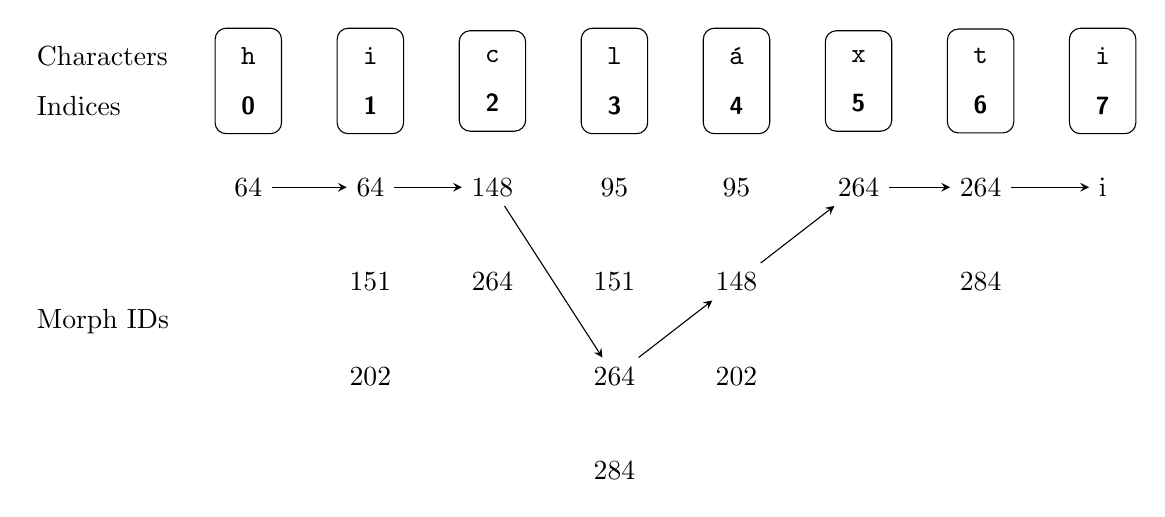
\begin{tikzpicture}[node distance=1.55cm, auto, >=stealth]
	\tikzstyle{annot}=[text width=15ex]
	\tikzstyle{reduced}=[text width=3ex]
\tikzstyle{block} = [rectangle, draw, text width=1em, text centered, rounded corners, minimum height=3em, inner sep=7pt]
  \node[annot](annot1) at (-1cm, 0cm){\vspace{3pt}Characters\vspace{3pt}\\Indices};
  \node[annot,below of=annot1] at (-1cm, -1.5cm)(annot2){Morph IDs};
    \node [block, right of=annot1] (idx0) {\vspace{3pt}\texttt{h}\vspace{3pt}\\\textsc{\small\textsf{\textbf{0}}}};
    \node [below of=idx0,node distance=1.35cm] (idx0-1) {64};
        \node [block,right of=idx0] (idx1) {\vspace{3pt}\texttt{i}\vspace{3pt}\\\textsc{\small\textsf{\textbf{1}}}};
    \node [below of=idx1,node distance=1.35cm] (idx1-1) {64};
    \node [below of=idx1-1,node distance=1.2cm] (idx1-2) {151};
    \node [below of=idx1-2,node distance=1.2cm] (idx1-3) {202};
            \node [block,right of=idx1] (idx2) {\vspace{3pt}\texttt{c}\vspace{3pt}\\\textsc{\small\textsf{\textbf{2}}}};
    \node [below of=idx2,node distance=1.35cm] (idx2-1) {148};
    \node [below of=idx2-1,node distance=1.2cm] (idx2-2) {264};
                \node [block,right of=idx2] (idx3) {\vspace{3pt}\texttt{l}\vspace{3pt}\\\textsc{\small\textsf{\textbf{3}}}};
    \node [below of=idx3,node distance=1.35cm] (idx3-1) {95};
    \node [below of=idx3-1,node distance=1.2cm] (idx3-2) {151};
    \node [below of=idx3-2,node distance=1.2cm] (idx3-3) {264};
       \node [below of=idx3-3,node distance=1.2cm] (idx3-4) {284};
                    \node [block,right of=idx3] (idx4) {\vspace{3pt}\texttt{\'{a}}\vspace{3pt}\\\textsc{\small\textsf{\textbf{4}}}};
    \node [below of=idx4,node distance=1.35cm] (idx4-1) {95};
    \node [below of=idx4-1,node distance=1.2cm] (idx4-2) {148};
    \node [below of=idx4-2,node distance=1.2cm] (idx4-3) {202};
                        \node [block,right of=idx4] (idx5) {\vspace{3pt}\texttt{x}\vspace{3pt}\\\textsc{\small\textsf{\textbf{5}}}};
    \node [below of=idx5,node distance=1.35cm] (idx5-1) {264};
                            \node [block,right of=idx5] (idx6) {\vspace{3pt}\texttt{t}\vspace{3pt}\\\textsc{\small\textsf{\textbf{6}}}};
    \node [below of=idx6,node distance=1.35cm] (idx6-1) {264};
    \node [below of=idx6-1,node distance=1.2cm] (idx6-2) {284};
                                \node [block,right of=idx6] (idx7) {\vspace{3pt}\texttt{i}\vspace{3pt}\\\textsc{\small\textsf{\textbf{7}}}};
    \node [below of=idx7,node distance=1.35cm] (idx7-1) {i};
\draw[->] (idx0-1) -- (idx1-1);
\draw[->] (idx1-1) -- (idx2-1);
\draw[->] (idx2-1) -- (idx3-3);
\draw[->] (idx3-3) -- (idx4-2); 
\draw[->] (idx4-2) -- (idx5-1); 
\draw[->] (idx5-1) -- (idx6-1); 
\draw[->] (idx6-1) -- (idx7-1); 
\end{tikzpicture}
\caption{Finding the optimal path through the morphs (morph IDs) associated with the word \textit{hicl\'{a}xti}}
% where morphs are represented by their IDs. A \emph{morph sequence} is a mapping from morphs to characters.}
\label{fig:best-paths}
\end{mdframed}
\end{figure}
The second major objective of Stage 3 is to abstract away from individual 
characters by eliminating repeated morph IDs. 
This is straightforward in cases of uninterrupted 
occurrences of the same morph ID, such as the consecutive 64s in \eqref{eq:best-path}. 
Consecutive morph IDs were simply mapped onto a \emph{single} instance of the same ID. Thus, for example,
\begin{equation*}
\texttt{64, 64} \quad \mapsto \quad \texttt{64}
\end{equation*}
However, sometimes optimal paths
exhibit morph interdigitation, as does our optimal path \eqref{eq:best-path}, in which morphs 148 and 264 are interleaved. 
%Because Morfessor does not deal 
%with interdigitation, 
Stage 3, however, collapsed sequences of interleaved morphs into two adjacent monolithic
morphs. That is,
\begin{equation*}
\texttt{148, 264, 148, 264, 264} \quad \mapsto \quad \texttt{148, 264}
\end{equation*}
Orphaned characters such as the \textit{i} in \eqref{eq:best-path} 
were retained in place. Thus, the abstracted, or compressed, version of path \eqref{eq:best-path} was
\begin{equation}\label{eq:reduced-best-path}
\texttt{hicl\'{a}xti} \quad \mapsto \quad \texttt{64, 148, 264, i}
\end{equation}
The final step within Stage 3 was to replace the morph IDs in the compressed paths 
with atomic unicode characters. Each morph ID was uniquely associated with a atomic unicode character, in particular, a character 
from the CJK (Chinese, Japanese, Korean) unicode block. The 
CJK correspondents of morph IDs 64, 148, and 264 
were as in figure~\ref{tab:morphs-chinese}.
\begin{figure}[t]
\setlength{\extrarowheight}{8pt}
\centering
\begin{tabular}{ccc}
\toprule
Morph ID & & CJK char \\
\midrule
64 & $\mapsto$ & \raisebox{-0.13cm}{
\includegraphics[scale=.3]{cjk-char-0-2}}\\
148 & $\mapsto$ & \raisebox{-0.13cm}{
\includegraphics[scale=.3]{cjk-char-0-1}} \\
264 & $\mapsto$ & \raisebox{-0.12cm}{
\includegraphics[scale=.3]{cjk-char-0-0}} \\
%i & $\mapsto$ & i \\
\bottomrule
\end{tabular}
\caption{Mapping morphs to atomic symbols from the CJK unicode block}
\label{tab:morphs-chinese}
\end{figure} 
These CJK characters along with the orphaned \textit{i} were joined together to form a single string as follows:
\begin{center}
\raisebox{-0.1cm}{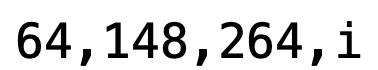
\includegraphics[scale=0.4]{reduced-morph-IDs}} \quad $\mapsto$ \quad \raisebox{-0.1cm}{
\includegraphics[scale=0.4]{cjk-sequence}} \quad $\mapsto$ 
\quad \raisebox{-0.10cm}{\includegraphics[scale=0.4]{conjoined-cjk-sequence}}
\end{center}
The experimental input files to Morfessor consisted of strings like \raisebox{-0.10cm}{\includegraphics[scale=0.4]
{conjoined-cjk-sequence}}. Figure~\ref{fig:morfessor-input} shows an excerpt from a Morfessor input file.

%repeated morph ID results in a doubling of the path's weight as long as the morph ID's immediately preceding instance is within three positions of the repeated instances
%
% Given a path of morph IDs, if a morph ID is repeated in the path, and if its recurrence is 3 or more  the  same morph ID is recurs within or fewer character positions let $\mu$ be one of morph IDs at index $n$. If $\mu$ is also present at indices $n-3$, $n-2$, or $n-1$ (i.e., within three preceding positions), the weight of this path is \textit{doubled}. That is, it is \emph{two times} the average of its component morphs.
%
%and/or positionfeatures weighting to morphs.  in which each feature (i.e., surface unit) was inherently 
%weighted by its reconstructed activity (see section~\ref{sec:mixing-fiction}), 
%and each morph's weight was then computed as the average of the activities of its component features.
%The sequence consists of a list of pairs; eachcharacter in a given word tio the morphs that 
%def update\_wt(weighted_sequence, morphID):
%		try: int\_ID = int(morphID)
%		except TypeError:
%			morph_obj = morphID
%			item_wt = 1.0
%		except ValueError:
%			morph_obj = morphID
%			item_wt = 1.0
%		else:
%			morph\_obj = morph\_dict[int\_ID][-1]
%			item\_wt = morph\_obj.get\_weight()
%		seq\_wt = weighted\_sequence[0]
%		sequence = weighted\_sequence[-1]
%		new\_avg = (seq_wt+item\_wt)/2.0
%		for n in range(1,3):
%			try: item = sequence[-n]
%			except IndexError: 
%				break
%			else:
%				if item == morphID:
%					return 2.0*new\_avg
%		return new\_avg
		
%\begin{figure}[ht]
%\centering
%\setlength{\extrarowheight}{8pt}
%\begin{tabular}{lcc}
%\toprule
%\text{Word} & \text{Morph ID} & \text{Char Indices} \\
%\midrule 
% \texttt{hicl\'{a}xti:} & & \\
%& \texttt{64} & \texttt{[0,1]} \\
%%\texttt{148:[2,4]} \texttt{[2,3,5,6]} \\
%%\texttt{64:[0,1]} \texttt{151:[1,3]} \texttt{148:[2,4]} \\ \texttt{284:[3,6]} 
%%\texttt{64:[0,1]} \texttt{2o2:[1,4]} \texttt{264:[2,3,5,6]}
%%\texttt{64:[0,1]} \texttt{148:[2,4]} \texttt{284:[3,6]}
% & \texttt{95:} & \texttt{[3,4]} \\
%  & \texttt{148:} & \texttt{[2,4]} \\
%   & \texttt{151:} &  \texttt{[1,3]} \\
%    & \texttt{202:} &  \texttt{[1,4]} \\
% & \texttt{264:} &  \texttt{[2,3,5,6]} \\
% & \texttt{284:} & \texttt{[3,6]} \\
% & \texttt{i:} & \texttt{[7]} \\
%\bottomrule
%\end{tabular}
%\label{fig:computing-mappings}
%\caption{Finding the optimal morph path.}
%\end{figure}



%We did not want overlapping segments within a single analysis; that is, within the same analysis,
%each character index 
%\begin{algorithm}[h]
%\KwData{\textbf{M}, \textbf{C}, \textbf{X}, \textbf{R}}
%\KwResult{Optimized \textbf{M} and \textbf{C} matrices}
%def update\_weight(self):
%		sum\_wt = 0.0
%		for my\_fwp in self.fwp\_list:
%			sum_wt += my\_fwp.get\_weight()
%		%try: self.weight = sum_wt/float(len(self.fwp_list))
%		%except ZeroDivisionError: self.weight = 0.0
%\label{alg:update-wt}
%\caption{The weight of a morph is computed as the average of the activities of its  component features.}
%\end{algorithm}
		
%def avg\_wt(morphID\_list, morph\_dict):
%	s = 0.0
%	\#print "avg_wt"
%	morph_objs = list\_of\_morph\_objs(morphID_list, morph_dict)
%	for morph_obj in morph_objs:
%		s += morph\_obj.get\_weight()
%	try: quotient = s/float(len(morph\_objs))
%	except ZeroDivisionError: return 0.0
%	else: return quotient

%STEPS: [(0, [64]), (1, [64, 151, 202]), (2, [148, 264]), (3, [95, 151, 264, 284]), (4, [95, 148, 202]), (5, [264]), (6, [264, 284]), (7, u'i')]
	
%In the case of (\ref{ex:mapping}), for example,-->  
%some morphs can be eliminated because they share character indices with other morphs. 
%In fact, redundant, overlapping morphs
%\emph{must} be reduced as much as possible. 

% After eliminating morphs \texttt{151}, \texttt{202}, and \texttt{284}, 
%we arrive at the following compressed sequence of morph IDs computed at the end of Stage 2
%is optimized and compressed to yield a single best path through the word. 
% the best sequence or ``path" and then compress it.
 %That is, remove repeated instances of the same morphID.
% \begin{figure}[ht]
% %\subfigure[(Reduced) mappings from morphs to characters\label{fig:char-indices-to-morph-IDs}]{
%\centering
%\setlength{\extrarowheight}{5pt}
%\begin{tabular}{lcc}
%\toprule
%\text{Word} & \text{Morph ID} & \text{Char Indices} \\
%\midrule 
% \texttt{hicl\'{a}xti:} & & \\
%& \texttt{64:} & \texttt{[0,1]} \\
% & \sout{\texttt{95:}} & \sout{\texttt{[3,4]}} \\
%  & \texttt{148:} & \texttt{[2,4]} \\
%   & \sout{\texttt{151:}} &  \sout{\texttt{[1,3]}} \\
%    & \sout{\texttt{202:}} &  \sout{\texttt{[1,4]}} \\
% & \texttt{264:} &  \texttt{[2,3,5,6]} \\
% & \sout{\texttt{284:}} & \sout{\texttt{[3,6]}} \\
% & \texttt{i:} & \texttt{[7]} \\
%\bottomrule
%\end{tabular}
%%}
%\label{fig:computing-mappings}
%\caption{The mapping from morph IDs to the characters (i.e., character indices) of the word
%\textit{hicl\'{a}xti} following the elimination of unmatched morphs}
%\end{figure}

%\begin{exe} \ex \label{ex:comp-with-indices} 
%hicl\'{a}xti \quad \texttt{64:[0,1], 148:[2,4], 264:[2,3,5,6], i}
%\ex %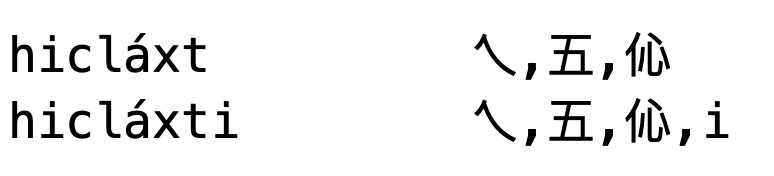
\includegraphics[width=.3\linewidth]{cjk-mappings-0}
%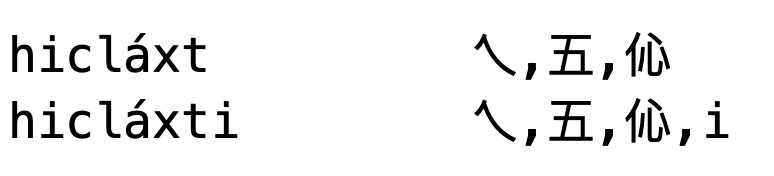
\includegraphics[scale=.3]{cjk-mappings-0}
%\end{exe}

%\begin{figure}[h]
%\centering
%%\includegraphics[width=.3\linewidth]{example-image}\quad
%\subfigure[Segmentation: Morphs and their constituent characters]{ 
%\centering
%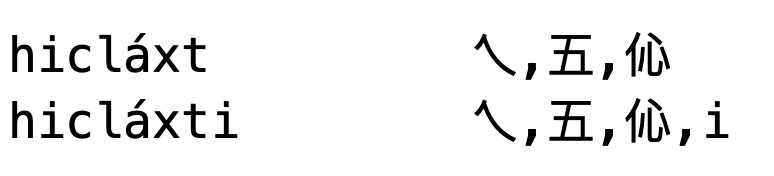
\includegraphics[width=.3\linewidth]{cjk-mappings-0}
%} \\[\baselineskip]
%\subfigure[Morphs mapped to CJK characters]{ 
%\centering
%\qquad \qquad 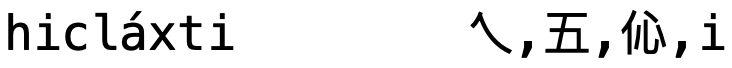
\includegraphics[width=.3\linewidth]{cjk-mappings-2}
%%\quad\includegraphics[width=.3\linewidth]{example-image-b}
%%\\[\baselineskip]% adds vertical line spacing
%%\includegraphics[width=.3\linewidth]{example-image}\quad\includegraphics[width=.3\linewidth]{example-image-a}\quad\includegraphics[width=.3\linewidth]{example-image-b}
%}
%\label{tab:morphs-chinese}
%\caption{Mapping morphs to atomic symbols from the CJK block of unicode characters}
%\end{figure}

%Note the \textit{i} at the end of the sequence. This is an ``orphan" alphabetic character that was never associated with a morph. Such stranded characters were not uncommon. They were retained so that every character would be accounted for.
%The idea is to abstract away from the individual characters as much as possible and allow morph to be a single, atomic entity, with no internal structure.] 
%The purpose of this stage, however, is to abstract away from the individual characters and treat each morph
%%as much as possible, so that each morph could be treated 
%as a single, atomic entity, with no internal structure.
%Thus, the compressed sequence in (\ref{ex:comp-with-indices}) would be look more like the following:
%\begin{exe} \ex \label{ex:comp-no-indices} 
%hicl\'{a}xti \qquad  $\to$ \qquad \texttt{64, 148, 264, i}
%\end{exe}
%The last step in Stage 3 is to \emph{encode} the morph-ID sequence in example (\ref{ex:comp-no-indices})by replacing each
%ID number with a unique, atomic unicode character---in particular, a character 
%from the CJK unicode block, as illustrated in figure~\ref{fig:map-and-replace}.
%The resulting sequence was then joined together to form a single string, as in 
%subfigure~\ref{subtab:cjk-replacement}.

% and then joining the characters together to form 
%a string, e.g., a four-character string in the case of (\ref{ex:comp-no-indices}).

%\begin{table}[ht!]
%\setlength{\extrarowheight}{6pt}
%\centering
%\begin{tabular}{ccc}
%\toprule
%Morph ID & & CJK char \\
%\midrule
%64 & $\to$ & \raisebox{-0.13cm}{
\includegraphics[scale=.3]{cjk-char-0-2}}\\
%148 & $\to$ & \raisebox{-0.13cm}{
\includegraphics[scale=.3]{cjk-char-0-1}} \\
%264 & $\to$ & \raisebox{-0.12cm}{
\includegraphics[scale=.3]{cjk-char-0-0}} \\
%i & $\to$ & i \\
%\bottomrule
%\end{tabular}
%\label{tab-cjk-mapping}
%\caption{Replacing morph (i.e., morph IDs) with CJK chars in the word \textit{hicl\'{a}xti}}
%\end{table}

%\begin{figure}[t]
%\centering
%\setlength{\extrarowheight}{6pt}
%\subfigure[Mapping\label{subtab:cjk-mapping}]{
%\centering
%\begin{tabular}{ccc}
%\toprule
%Morph ID & & CJK char \\
%\midrule
%64 & $\to$ & \raisebox{-0.13cm}{
\includegraphics[scale=.3]{cjk-char-0-2}}\\
%148 & $\to$ & \raisebox{-0.13cm}{
\includegraphics[scale=.3]{cjk-char-0-1}} \\
%264 & $\to$ & \raisebox{-0.12cm}{
\includegraphics[scale=.3]{cjk-char-0-0}} \\
%i & $\to$ & i \\
%\bottomrule
%\end{tabular}
%} \\
%%\label{tab-cjk-mapping}
%\subfigure[In Stage 3, the morphs in the word \textit{hicl\'{a}xti} are replaced by atomic CJK characters.\label{subtab:cjk-replacement}]
%{
%\centering
%%\begin{tabular}{ccc}
%%\toprule
%%Morph ID & & CJK char \\
%%\midrule
%%hicl\'{a}xti & $\to$ & hicl\'{a}xti \\
%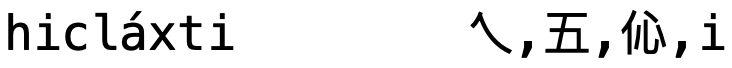
\includegraphics[scale=.3]{cjk-mappings-2}
%%64 & $\to$ & \raisebox{-0.13cm}{
\includegraphics[scale=.3]{cjk-char-0-2}}\\
%%148 & $\to$ & \raisebox{-0.13cm}{
\includegraphics[scale=.3]{cjk-char-0-1}} \\
%%264 & $\to$ & \raisebox{-0.12cm}{
\includegraphics[scale=.3]{cjk-char-0-0}} \\
%%i & $\to$ & i \\
%%\bottomrule
%%\end{tabular}
%}
%\label{tab:map-and-replace}
%\caption{Subfigures~\ref{subtab:cjk-mapping} and \ref{subtab:cjk-replacement}, baby!}
%\end{figure}

%\begin{figure}[t]
%\centering
%%\includegraphics[width=.3\linewidth]{example-image}\quad
%\subfigure[Segmentation: Morphs and their constituent characters]{ 
%\centering
%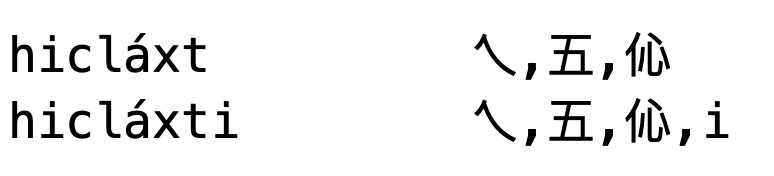
\includegraphics[width=.3\linewidth]{cjk-mappings-0}} \\
%[\baselineskip]
%\subfigure[Morphs mapped to CJK characters]{ 
%\centering
%\qquad \qquad 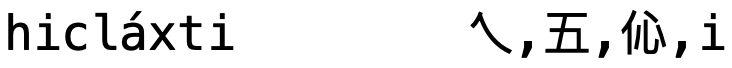
\includegraphics[width=.3\linewidth]{cjk-mappings-2}}
%%\quad\includegraphics[width=.3\linewidth]{example-image-b}
%%\\[\baselineskip]% adds vertical line spacing
%%\includegraphics[width=.3\linewidth]{example-image}\quad\includegraphics[width=.3\linewidth]{example-image-a}\quad\includegraphics[width=.3\linewidth]{example-image-b}
%\end{figure}

\begin{figure}[t] 
\centering
\begin{mdframed}
\vdots \vspace{6pt}
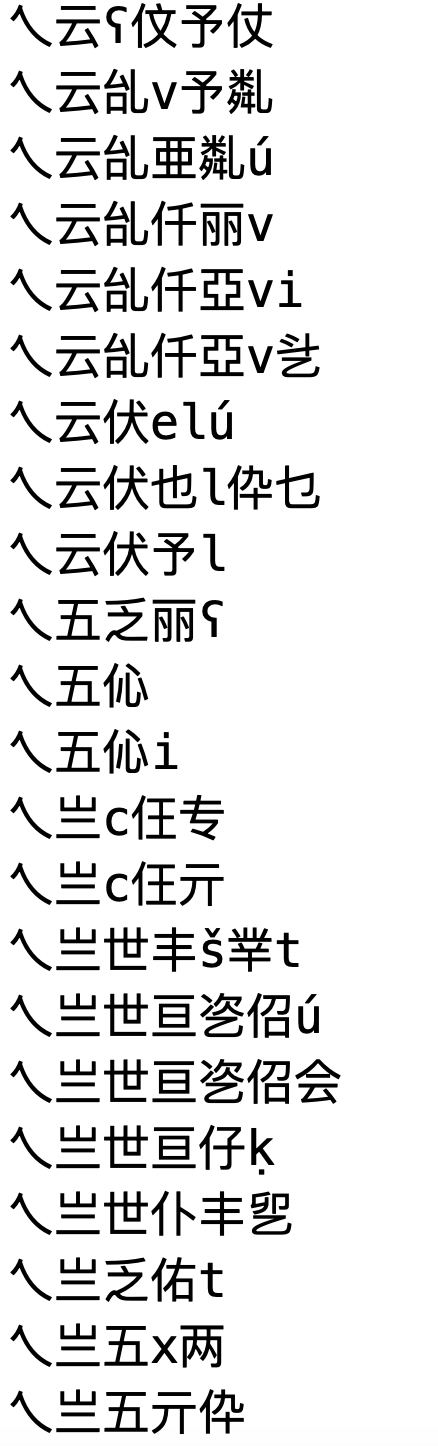
\includegraphics[scale=0.3]{input-to-morfessor-1} \\
\vdots
%\label{fig:morfessor-input}
\caption{Excerpt from a Morfessor input file} 
\label{fig:morfessor-input}
\end{mdframed}
\end{figure}

 
\subsubsection{\textsc{stage 4:} Decompress and evaluate}
 In Stage 4, the final stage, 
 Morfessor was fed both the experimental and control files for each experimental trial---i.e.,
 each combination of $\delta$ and $s$ values (see chapter~\ref{ch:experi}).
Morfessor then output a \textit{segmentation} file for both types of input file; that is, it
produced both an experimental and a control segmentation for 
each $\delta$ and $s$ valuation. 
Figure~\ref{fig:morfessor-output} 
shows an excerpt from an 
experimental segmentation file. The `+' signs indicate 
the boundaries between the morphological segments that Morfessor induced. 
Note that many of the
Morfessor-induced segments in figure~\ref{fig:morfessor-output} consist of multiple 
CJK characters. Since each CJK character corresponds to a morph, 
this means that many of the Morfessor-induced segments consisted of multiple
MCMM-induced morphs.

\begin{figure}[t]
%\centering
\begin{mdframed}
\vdots \vspace{6pt}
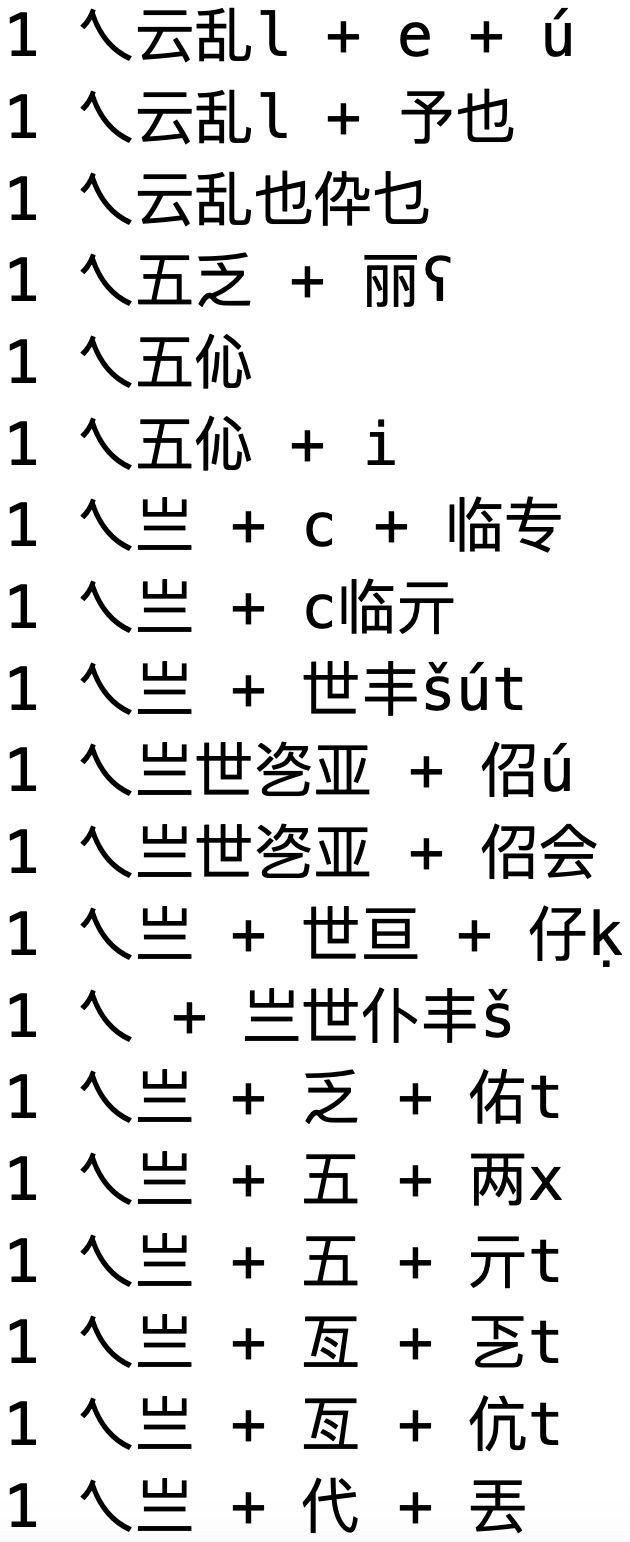
\includegraphics[scale=0.3]{output-from-morfessor-0} \\
\vdots
\caption{Excerpt from a Morfessor output file}
\label{fig:morfessor-output}
\end{mdframed}
\end{figure}
 %Morfessor then output an experimental and a control model. 
%  each representing a segmentation model), one control and one experimental, the latter still consisting of encoded words, except that the encoded words are now segmented.
% original (or ``normal") words, while the other comprised segmentation of the encoded versions of the original words. 
 %Note, however, that even the encoded words of the experimental file had started out as original words, they so altered in their encoded forms that they generally bore no resemblance to their original forms.
% described  computes a segmentation for each compressed/encoded word in the experimental set. We also run Morfessor on the control dataset, thus obtaining segmentations of the original words. We at this point have two segmented files, but the words in the experimental file are still encoded. 
%A ten percent sample of the data was previous  10 percent sample of these segmented compressed words and \emph{decompress} them, i.e.,
Both the experimental and control models had to be evaluated against the same gold standard.\footnote{Note also that each
pair of $s$ and $\delta$ values yielded a different word coverage
and thus 
each required its own control model.}
But to make this possible, Stage 4 first had to \emph{decode} (or \emph{decompress}) the strings in the experimental segmentation file; that is, it had to take experimental-string segmentations like the ones in 
figure~\ref{fig:morfessor-output} and convert the CJK characters back to the original character sequences.
To avoid altering Morfessor’s segmentation decisions, 
each morfessor-induced segment 
%(consist of multiple morphs) 
was decoded separately. The decoded segments were then reassembled. 
Morfessor's built-in evaluation utility was used to evaluate each model against the gold standard. 
For example, 
in the case of \textit{hicl\'{a}xti}, %our example word throughout this section, 
Morfessor was given the encoded string 
\begin{center}
\raisebox{-0.08cm}{\includegraphics[scale=0.4]{conjoined-cjk-sequence}}
\end{center}
and output the \emph{segmented} encoded string
\begin{center}
\raisebox{-0.08cm}{\includegraphics[scale=0.37]{segmented-encoded-string}}
\end{center}
whose first segment comprised the three  
CJK symbols corresponding to the morphs 64, 148, and 264, 
and the second segment was the \emph{i}. In the final decoding process, 
the morphs 64, 148, and 264 together (i.e., as a single segment) mapped onto the string \textit{hicl\'{a}xt}, 
and thus Morfessor's segmentation became \textit{hicl\'{a}xt + i}.
The same process was carried out for each word in the experimental segmentation file and the entire file was thus decoded. At this point, the words in the experimental segmentation file once again shared the same characters as their control counterparts.
%That is, each
%segment in experimental segmentation file was decoded separately in order to preserve Morfessor's segmentation decisions.
 %decoding process did not  placement of the  `+' signs remained distinct.
The decoded experimental segmentations and the control segmentations were then evaluated against the same gold-standard data set, which I created by manually segmenting 
one-tenth of the original, unprocessed wordlist. 
This was repeated for each experimental trial, i.e., for each of the $\delta$ and $s$ 
pairs as well as for each of the three data types (i.e., orthographic, transcriptions with stress, 
and transcriptions without stress).
I created a separate gold-standard file for each data type.

\section{Summary}
We began this chapter by pointing out that there is at present no single ideal way to evaluate Multimorph's output.
We thus adopted a multi-faceted approach to the evaluation, one that included both a qualitative and
a quantitative component. Moreover, the quantitative component had two complementary components, namely an intrinsic component and an extrinsic component. Most of this chapter focused on describing the intrinsic and the extrinsic evaluation procedure. Both involved considerable processing. 

The instrinsic evaluation required a set of gold-standard morphological word-to-morphological-category mappings. We took the morphological analyses from the Berman Longitudinal Corpus to serve gold-standard class assignments, since we lacked a gold-standard set of morph or morphome mappings. However, we had to modify these categories considerably, mapping them onto categories that were based more closely on form rather than abstract morphosyntactic category. These mappings were limited, though, since, if taken to an extreme, they would become tantamount to carrying out an morph/morphome annotation from scratch.

The extrinsic evaluation regarded Multimorph as an intermediate step in a larger process. It tested the hypothesis that Multimorph could ``pre-digest'' a wordlist for Morfessor and thus improve Morfessor's performance on that
wordlist.

In the next chapter, we examine the results of these evaluation approaches.


%   \item Mapping from features to prefix characters:
%   \begin{enumerate}
       %\ex \label{ex-1a} 
%       \item If there are at least two features of the form \texttt{a<b} and \texttt{a<c}, such that \textit{b} $\ne$ \textit{c}, then \textit{a} is at least part of a prefix. But what if the precedence features have an abstract component, as in the following?
%       \begin{itemize}
%       \item \texttt{x<C}
%       \item \texttt{x<V}
%       \end{itemize}
%       How does one determine inequality between abstract characters? Answer: C $\ne$ V. So there can still be inequality, just less of it. 
       %If there is additionally a bigram feature \texttt{a+t} or \texttt{t+a}, such that \textit{t} $\ne$ \textit{b}, \textit{t} $\ne$ \textit{c} (see above), then the prefix is either \textit{at-} or \textit{ta-}, respectively. 
%       \ex When there is a character \textit{a} satisfying rule \ref{ex-1a} has more than one character can only be determined by \emph{bigram} features. In particular, if there is additionally a bigram feature \texttt{a+t} or \texttt{t+a}, such that \textit{t} $\ne$ \textit{b}, \textit{t} $\ne$ \textit{c} (see above), then the prefix is either \textit{at-} or \textit{ta-}, respectively.
       %\ex 
%       \item If there is at least one positional feature of the form \texttt{a@[}$x$\texttt{]}, where $x$ is a positive integer, then \textit{a} is at least part of a prefix. If there are two or more consecutive positional features, i.e., features like \texttt{a@[}$x$\texttt{]}, \texttt{b@[}$x+1$\texttt{]}, \texttt{c@[}$x+2$\texttt{]}, and so on, then the prefix is the entire string of characters indicated by these features.
%    \end{enumerate}
%
%  \item Mapping from features to suffix characters:
%   \begin{enumerate}
%   \item If there are at least two features of the form \texttt{b<a} and \texttt{c<a}, such that \textit{b} $\ne$ \textit{c}, then \textit{a} is at least part of a suffix. If there is additionally a bigram feature \texttt{a+t} or \texttt{t+a}, where \textit{t} is a different character than either \textit{b} or \textit{c} (see above), then the prefix is either \textit{-at} or \textit{-ta}, respectively.
%
%   \item If there is at least one positional feature of the form \texttt{a@[}$x$\texttt{]}, where $x$ is a negative integer, then \textit{a} is at least part of a suffix. If there are two or more consecutive positional features, i.e., features like \texttt{a@[}$x${]}, \texttt{b@[}$x-1${]},\texttt{ c@[}$x-2${]}, and so on, then the suffix is the entire string of characters indicated by these features.
%   \end{enumerate}
%  \item If a cluster centroid has conflicting active features, then the cluster is void; it does not correspond to any morph.
%\end{enumerate}
%%EXAMPLES
%
%\begin{exe}
%%Cluster #0 from 3_3_1_K-50_N-6888_2015-01-24_14-48
%\ex Active features: e+w (1.0), e+i (1.0), l@[0] (1.0), e@[0] (1.0), e$<$w (0.9713), l+w (0.9466), e$<$i (0.8878), l<w (0.7655), e@[1] (0.7321), e+t (0.7049) \\
%Morph: None \\
%Pertinent rule: 4
%%
%%Cluster #2 from 3_3_1_K-50_N-6888_2015-01-24_14-48
%\ex Active feature: w+i (1.0), l+i (1.0), i+m (1.0), i+i (1.0), w$<$i (1.0), i@[-2] (1.0), m@[-1] (1.0), l<i (0.9941), i<i (0.8206), l+m (0.7164) \\
%Morph: -liim (suffix) \\
%Pertinent rule: 3b
%%
%%Cluster #5 from 3_3_1_K-50_N-6888_2015-01-24_14-48
%%Active features: m+i (1.0), i+m (1.0), m<i (1.0), i@[-2] (1.0), m@[-1] (1.0), m+m (0.9825), m@[0] (0.8077), w+m (0.7786), m+w (0.7006), m<m (0.6840)
%%Morph: None
%%Pertinent rule: 4
%%
%%Cluster #6 from 3_3_1_K-50_N-6888_2015-01-24_14-48
%\ex Active features: b@[0] (1.0), b$<$w (0.9285), b$<$i (0.9232), b+t (0.6000), b+r (0.5867), b$<$t (0.4608), b+m (0.4576), b@[1] (0.4512) \\
%Morph: b- (prefix) \\
%Pertinent rules: 2a and 2b 
%%
%%Cluster #13 from 4_star_K-350_N-_2014-07-20_03-45.K@303
%\ex Active features: p$<$q (1.0), p$<$d (0.9999), q$<$d (0.9999) \\
%Morph: p.q.d. (root)  (The feature p*d is not relevant, as it turns out.) \\
%Pertinent rule: 1b
%%
%%Cluster #1 from 4_star_K-350_N-_2014-07-20_03-45.K@303
%\ex Active features: w$<$t (1.0), w@[-2] (1.0), t@[-1] (1.0) \\
%Morph: -wt (suffix) \\
%Pertinent rule: 3b
%%
%%Cluster #26 from 4_star_K-350_N-_2014-07-20_03-45.K@303
%\ex Active features: r$<$i (0.99), r@[-3] (0.98), r+i (0.96), i@[-2] (0.9), i+r (0.84), r+m (0.8), h+r (0.8), r$<$m (0.79), r+t (0.74), w+r (0.68) \\
%Morph: None (There are active features for both a prefix and a suffix.) \\
%Pertinent rule: 4
%%
%%Cluster #184 from 4_star_K-350_N-_2014-07-20_03-45.K@303
%\ex Active feature: p$<$g (1.0) \\
%Morph: None \\
%Pertinent rule: 1b 
%%
%%Cluster #201 from 4_star_K-350_N-_2014-07-20_03-45.K@303
%\ex Active features: x$<$z (1.0), z$<$q (0.98) \\
%Morph: x.z.q. (root) \\
%Pertinent rule: 1b
%%
%%Cluster #219 from 4_star_K-350_N-_2014-07-20_03-45.K@303
%\ex Active features: d$<$h (1.0), h$<$z (1.0), z$<$d (0.99), z$<$t (0.99) \\
%Morph: None \\
%Pertinent rule: 4
%\end{exe}
%
%Via Chinese: Every symbol in an encoded morfessor segment is itself a distinct morph.
%
%\subsubsection{Stage 2: Match morph characters to word characters} Once a morph has been gleaned from a cluster's centroid vector, the characters of the morph must be matched to the corresponding characters in the cluster's member words. 
%
%The $\mathbf{M}$ matrix contains the cluster activities for each word. By consulting $\mathbf{M}$, we can ascertain the set of clusters to which each cluster belongs. Each cluster can be thought of as essentially equivalent to a particular morph, since the identities of morphs come from clusters. Indeed, Stage 1 ``extracts" from each cluster a $K$-length vector that  contains the key alphabetic characters associated with the cluster. Thus, via the cluster activities, each word is mapped to its set of morphs.
%
%At this point we will know which morphs are associated with each word, but we do not yet know the order of the morphs in words with more than one. Additionally, we will know, for each morph, whether it is a prefix ($P$), suffix ($SU$), or stem-component ($ST$). For example, suppose that the word \textit{whxlwm} (`and the dream') belongs to four clusters, namely those corresponding to the morphs \texttt{w}_{P}, \texttt{h}_{P}, \texttt{xlm}_{ST}, \texttt{w}_{ST}, where the subscripts $P$ and $ST$ stand for \textit{prefix} and \textit{stem-component}, respectively.
%
%First, the prefixes are matched to word characters. Then stem-components are matched, and finally any suffixes are matched (there are no suffixes in the present example). Whenever a morph character matches a word character, the word character is popped from the word, and the morph character is popped from the morph. The word character is then linked to the morph in question. 
%
%Thus, in our example, the matching algorithm proceeds as follows: First, each of the prefixes \texttt{h}_{P} and \texttt{w}_{P} (the order should not matter) are compared to the first character of \textbf{whxlwm}. The \texttt{w}_{P} matches, so we get \{ \texttt{w}_{P}:\texttt{w} \}. The \texttt{w} is popped 
%
%from \textbf{whxlwm} as well as from \texttt{w}_{P}, thus completing the prefix morph \texttt{w}_{P} and removing it from consideration. Next, \texttt{h}_{P} (the only remaining prefix) is matched to the \texttt{h} of \textbf{hxlwm}, leaving us with \{  \texttt{w}_{P}:\texttt{w} \texttt{h}_{P}:\texttt{h} \}, \textbf{xlwm}, and no more prefixes.
%
%Now only the stem-components remain. \texttt{w}_{ST} fails to match the first character 
%of \textbf{xlwm}. However, the \texttt{m} of \texttt{xlm}_{ST} does, yielding
% \{ \texttt{w}_{P}:\texttt{w} \texttt{h}_{P}:\texttt{h}, \texttt{xlm}_{ST}:m\}, 
% \textbf{lwm}, an stem-components {\texttt{lm}_{ST} and \texttt{w}_{ST}. 
% The \texttt{q} of {\texttt{lm}_{ST} matches the \texttt{q} in \textbf{qm}, giving us 
% \{\texttt{w}_{P}:\texttt{w} \texttt{h}_{P}:\texttt{h}, \texttt{xlm}_{ST}:\texttt{mq}\}, 
% \textbf{wm}, and stem-components \texttt{m}_{ST} and 
% \texttt{w}_{ST}. Next, \texttt{w}_{ST} matches the \texttt{w} in \textbf{wm}, 
%completing the stem-component \texttt{w}_{ST}. We now have \{\texttt{w}_{P}:\texttt{w} \texttt{h}_{P}:\texttt{h}, \texttt{xlm}_{ST}:\texttt{mq}, \texttt{w}_{ST}:\texttt{w}\}, \textbf{m}, and  
% \texttt{m}_{ST}.
% Finally, \texttt{m}_{ST} matches \textbf{m}, completing \{\texttt{xlm}_{ST}\} and consuming the word's last remaining character.
%%	\begin{verbatim}
%%		.*(x).*(\u00F3).?.?(t).*
%%	\end{verbatim}
%%	\texttt{.*(x).*(\'{o}).?.?(t).*}
%\subsubsection{Stage 3: Compress}. Here, each morph to an atomic symbol, 
%so that, e.g., a three-character morph becomes in effect single-character item, 
%as do all morphs consisting of more than one character. In this way, most of 
%the words is shortened (in terms of character-count) and thus compressed.
%Each atomic morph symbol is a unique unicode character. For example, 
%consider the 
%Hebrew words \textit{magdil} and \textit{gadol}, which share the root 
%\textit{g.d.l}. 
%Suppose that the Stage 2 outputs for these words are as in \eqref{ex:magdil} and 
%\eqref{ex:gadol}, respectively. 
%\begin{exe}  \ex \label{ex:unicode} \begin{xlist}
%	\ex magdil \quad ma-, \,\, g.d.l, \,\, i 
%	\label{ex:magdil}
%	\ex gadol \, \quad  g.d.l, \,\, a.o
%	\label{ex:gadol}
%	\end{xlist}
%\end{exe}
%Altogether, there are four \emph{unique} morphs in \eqref{ex:unicode}, namely \textit{ma-}, \textit{g.d.l}, 
%\textit{i}, and \textit{a.o}.
%Stage 3 will map each of these to a unique symbol, as in \eqref{ex:map}, for instance.
%\begin{exe}
%	\ex  \textit{ma-} $\mapsto$ \$ \quad \textit{g.d.l} $\mapsto$ \% \quad
%\textit{i} $\mapsto$ \& \quad \textit{a.o} $\mapsto$ \#
%\label{ex:map}
%\end{exe}
%Finally, each word is reassembled with atomic symbols being substituted for the morphs. 
%They are put together in the original order of their corresponding morphs.
%\begin{exe}  
%	\ex \label{ex:reassembled} \begin{xlist}
%	\ex magdil \quad \$\%\&
%	\label{ex:re-magdil}
%	\ex gadol \, \quad \%\#
%	\label{ex:re-gadol}
%	\end{xlist}
%\end{exe}
%% The atomic symbols are put together in the order of their corresponding character sequences, as illustrated in \eqref{ex:reassembled}. 
%Note, however, that in the case of interdigitation, the relative order of atomic symbols corresponding to interleaved sequences must be decided arbitrarily.
%
%\subsubsection{Stage 4: Test} 
%Two input files, a test and a 
%control file, are now fed to Morfessor. 
%The test file is the output of Stage 3.  %will contain the test data, i.e., the compressed words from Stage 3. 
%The control file consists of the original, unaltered words; its purpose is to serve as a baseline for measuring the effect 
%of the compression carried out in Stage 3. 
%% But what gives
%The idea here is to see if the MCMM's morphs, 
%now represented as atomic symbols, aide the 
%process of morphological segmentation.  % But how can we tell if the atomic symbols help?
%% What are they supposed to help?  Are they supposed to aide in the process of discovering the actual morphemes (i.e., the non-compressed, non-reduced morphemes)? If so, we need to somehow translate atomic symbols back into character sequences, but retaining the segmentation divisions computed on the strings of atomic symbols.
%Morfessor induces morphological segmentations for each file, yielding a \emph{control segmentation} and a \emph{test segmentation}. The words in the test segmentation at this point still consist of the atomic symbols from Stage 3. Without disrupting Morfessor's segmentation decisions, the atomic symbols were converted back into morphs (i.e., Stage 3 was undone).
%\begin{exe}
%	\ex   \$ $\mapsto$  \textit{ma-}
%	\quad \% $\mapsto$ \textit{g.d.l} 
%	\quad  \& $\mapsto$ \textit{i}
%	\quad  \# $\mapsto$ \textit{a.o}
%\label{ex:map}
%\end{exe}
%\begin{exe}  
%	\ex \label{ex:reassembled} \begin{xlist}
%	\ex  \$ \, + \, \% \, + \,  \& \quad $\mapsto$ \quad  ma \,+ \, gdl  \, + \, i
%	\label{ex:reconverted-magdil}
%	\ex  \% \, + \, \# \quad $\mapsto$  \quad gdl \, + \, ao
%	\label{ex:reconverted-gadol}
%	\end{xlist}
%\end{exe}
% The result is a test segmentation file whose words have the same characters as those of the control file, but possibly quite different segmentations. The two segmentations were evaluated against a common gold standard.
%%That is, do they make the task easier? 
%%Do they improve segmentation accuracy? 
%%Morfessor %then
%% induces morphological segmentations for each file, yielding a \emph{control segmentation} and a \emph{test segmentation}. The words in the test segmentation will at this point still consist of the atomic symbols from Stage 3. Without disrupting Morfessor's segmentation decisions, change the atomic symbols back to morphs (i.e., undo Stage 3). Finally, evaluate the two segmentations against a common gold standard.
%
%\subsection{Gold-standard data}
%Recall that Morfessor is a nonlinear \emph{sequential} algorithm; that is, it possesses nonlinearity, but not nonsequentiality (see section~\ref{sec:nls})
%and is thus incapable of detecting non-concatenative roots and patterns. 
%Moreover, interdigitation is lost when atomic symbols are substitute for character sequences. 
%Two basic types gold-standard data were therefore required: one to assess Morfessor's output and one to evaluate the 
%stem-internal root-and-pattern morphology.
% 
%\paragraph{Morfessor gold standard}
%%I will need gold-standard segmentations against which to assess Morfessor's output.  
%Morfessor produces two output (or analysis) files, one for the test file (processed words) and one for the control file (original or uprocessed words)
%To obtain gold-standard datasets for Morfessor, I manually segmented $\frac{1}{10}$ of the original, unprocessed wordlist.
%This amounts to a total of three unprocessed wordlists: a list of transcribed words, a list of transcribed words with stress marked, and a list of words spelled according to orthographic conventions. 
%
%\paragraph{Non-concatenative gold standard}
%To evaluate my system's performance on non-concatenative morphology, I need gold-standard roots for both the transcribed wordlists and the orthographic data. For the transcribed data, I extracted root annotations from the CHILDES morphological analyses. 

%For the orthographic wordlist, I will take advantage of the root annotations provided in the original dataset of \cite{daya-et-al:2008} (see section~\ref{sec:data}).
% 
%\paragraph{Gold-standard annotation}
%How are we going to figure this out? The control will serve as the baseline. 
%But we also need a gold standard segmentation to provide a frame of reference for comparing the test and control segmentations. 
%That is, the respective accuracies of the test and control segmentations 
%is measured with respect to the gold standard.

%How large does the gold-standard set need to be? 1000 words? 1/10 of the total data set?

%\subsection{Ancillary (Gold-Standard-Based) Evaluation}
%This evaluation will involve mapping \textsc{mila-ma}'s categories onto different sets of gold-standard classes. How will these sets differ? The idea, I guess, is to use sets with varying amounts of granularity, or different amounts of modification, or perhaps different types of modification.
%For example, do we want the categories to create a strict partition? Maybe the gold-standard classes could/should overlap.
%
%An MCMM clusters its input vectors (= words) according to shared hidden-unit activations. 
%Its clusters overlap one another; i.e.,
%a single word can belong to several clusters at once. % because a word can contain multiple morphemes. 
%%Evaluating overlapping clusters is more complicated than evaluating disjoint clusters. 
%To evaluate these clusters,
%I will use the measures \emph{BCubed Precision} and \emph{BCubed Recall}, 
%which are specially designed for overlapping clusters \citep{amigo-et-al:2009}.
%%Precision and recall evaluate a system's output against an external gold standard. 
%
%I will use a
%finite-state morphological analyzer, namely the MILA Morphological Analysis tool (\textsc{mila-ma}) 
%\citep{hebrew-resources:2008} to generate gold-standard classes. It is, however, non-trivial to apply \textsc{mila-ma} to this purpose.
%is not entirely straightforward. First, there is the general problem of evaluating an unsupervised clustering algorithm
%against external criteria. One usually has an idea about what the output should be, 
%but without a training set,
%it is difficult to be specific about this. 
%Second, one must consider that
%\textsc{mila-ma}'s particular categories may not be appropriate for cluster evaluation in every case.
%
%For example, \textsc{mila-ma} tends to use atomic categories such as \textsc{masc} and \textsc{pl} as opposed to \textsc{masc.pl}. In the case of Hebrew, \textsc{masc} and \textsc{pl} are abstract because neither corresponds to an actual morpheme. That is, the Hebrew \textsc{masc.pl} suffix \textit{-im} is fusional; it cannot be split into separate \textsc{masc} and \textsc{pl} substrings (cf. \textsc{masc.sg} forms, 
%which have no ending, and the \textsc{fem.pl} suffix \textit{-wt}).
%A clustering algorithm would be 
%disinclined to treat \textsc{masc} and \textsc{pl} as \textsc{mila-ma} does, since this would mean creating separate \textsc{masc} and \textsc{pl} clusters  despite the lack of a \emph{particular} \textsc{masc} suffix and a \emph{particular} \textsc{pl} suffix.
%%lack of shared formal elements. clusters because such clusters would not be based on shared formal elements; \textsc{masc} 
%%would contain words ending in -$\emptyset$ and \textit{-im}, and \textsc{pl} would contain words ending in \textit{-wt} and \textit{-im}.
%For this and similar reasons, \textsc{mila-ma}'s categories will need to be mapped to a somewhat adapted set 
%of gold-standard classes.

%****************
%\begin{description}
%\item[Stage 1: Extract.] Derive morphs from cluster centroids. That is, for each cluster centroid vector,  map the \emph{active} features to a particular sequence of alphabetic characters. The mappings is governed by a set of mapping rules. The resulting sequence of alphabetic characters is the morph. Repeat this process for each cluster (i.e., cluster centroid).
%
%\textbf{Example:} Suppose that \texttt{z<k} and \texttt{k<r} are the active features in a given cluster's centroid. These features would map to the (potentially discontinuous) character sequence \textit{zkr}. The morph would thus be the root \textit{z.k.r}.
%
%\item[Stage 2: Match.] Map morph characters to word characters. That is, given a cluster and its morph (obtained in Stage 1), go through the cluster's words, and in each word, determine which characters are the morph's characters. Label these characters as components of the morph in question. Repeat this process for each cluster/morph.
%Each morph is a (possibly discontinuous) sequence of alphabetic characters. 
%Given a cluster and its newly extracted morph, identity the morph's characters in each of the clusters words. 
%That is, for each word, match the morph's characters to the \emph{correct} word characters. Note that there is potential for ambiguity here. Suppose, for example, that the morph in question is the \textit{-wt}. It's easy enough to find a single \texttt{t} in a string of letters, but \texttt{t} is a frequently occurring letter, and it could easily occur elsewhere in the word. I have to make sure my matching algorithm selects the right character in cases like this. Repeat this process for each cluster. 
%For each word $w$ in a given cluster, identify the characters in $w$ that correspond to the morph's characters. counterparts of each the morph characters to their counterpart character in the word in question. with their matching characters in the word in 
%the characters of the morph to the corresponding characters in the cluster's member words.
%
%\paragraph{Example:}  
%Consider a cluster whose member words are \textit{mazkir}, \textit{hizkir}, \textit{zoker}, \textit{zokrim}, and \textit{zikron}. The morph in this case is the root \textit{z.k.r}. Stage 2 identifies the root consonants in each word and labels them as components of the morph \textit{z.k.r}. Here, the morph's characters are ``labeled" via boldface type:
%%\footnote{In reality, of course, a larger and more sophisticated labeling/indexing system is necessary, as every morph will require a distinct label/index.}:  
%\textit{ma\textbf{zk}i\textbf{r}},
%\textit{hi\textbf{zk}i\textbf{r}}, \textit{{z}o\textbf{k}e\textbf{r}}, \textit{\textbf{z}o\textbf{kr}im},
%and \textit{\textbf{z}i\textbf{kr}on}.
%The process is repeated for each cluster/morph.
%
%\item[Stage 3: Compress.] Map each morph to a single unique unicode character.
%\textbf{Example:} Consider the 
%Hebrew words \textit{magdil} and \textit{gadol}, which share the root \textit{g.d.l}. 
%Suppose that the Stage-2 outputs for these words are as in \eqref{ex:magdil} and \eqref{ex:gadol}, respectively. 
%\begin{exe}  \ex \label{ex:unicode} \begin{xlist}
%	\ex magdil \quad ma-, \,\, g.d.l, \,\, i 
%	\label{ex:magdil}
%	\ex gadol \, \quad  g.d.l, \,\, a.o
%	\label{ex:gadol}
%	\end{xlist}
%\end{exe}
%Altogether, there are four \emph{unique} morphs in \eqref{ex:unicode}, namely \textit{ma-}, \textit{g.d.l}, 
%\textit{i}, and \textit{a.o}.
%Each of these is mapped to a unique atomic symbol, as in \eqref{ex:map}.
%\begin{exe}
%	\ex  \textit{ma-} $\mapsto$ \$ \quad \textit{g.d.l} $\mapsto$ \% \quad
%\textit{i} $\mapsto$ \textit{i} \quad \textit{a.o} $\mapsto$ \#
%\label{ex:map}
%\end{exe}
%%Let the atomic symbols inherit the sequential order of their counterpart morphs. 
%In general, the atomic symbols inherit the ordering of the original morphs. 
%The exceptional cases are those of interdigitation. When two morphs are interleaved, 
%they are unordered with respect to each other.
%However, when they are mapped to atomic symbols, they necessarily 
%take on an arbitrary relative order because there is no way to interleave two 
%\emph{atomic} units: either $A$ precedes $B$ or $B$ precedes $A$; 
%there is no other option.
%%but with the atomic symbols now taking the places of of the original morphs. Put the symbols in the same order as their morph counterparts.  hat for morphs that are two or more characters long.. They are put together in the same order as the original morphs. This reducing or elsince it replaces whole character sequences, even discontinuous ones, with atomic symbols (see section~). 
%\begin{exe}  
%	\ex \label{ex:reassembled} \begin{xlist}
%	\ex magdil \quad \$\%\textit{i}
%	\label{ex:re-magdil}
%	\ex gadol \, \quad \%\#
%	\label{ex:re-gadol}
%	\end{xlist}
%\end{exe}
%%Now, when the characters of the two morphs are interleaved, i.e. in the case of interdigitation, the relative order of the morphs is indeterminate. However, when these two morphs are mapped to atomic symbols, they necessarily take on an arbitrary relative order. That is, either $A$ precedes $B$ or $B$ precedes $A$; there is no other option. 
%The mapping from morphs to atomic symbols thus abstracts interdigitation.  
%
%\item[Stage 4: Test.]
%%-- concatenative morphs.]
%Feed both the control file (i.e., the file containing the original wordlist) and the test file (i.e., the output of Stage 3) to
%Morfessor \citep{creutz-and-lagus:2005, creutz-and-lagus:2007}. Morfessor then induces morphological segmentations for each input file, yielding a \emph{control segmentation} and a \emph{test segmentation}. The words in the test segmentation will at this point still consist of the atomic symbols from Stage 3. Without disrupting Morfessor's segmentation decisions, change the atomic symbols back to morphs (i.e., undo Stage 3). Finally, evaluate the two segmentations against a common gold standard.
%%control file, will 
%%%now be fed to Morfessor. 
%%The test file is the output of Stage 3.  The control file will contain the original, unaltered words. 
%%It will provide a baseline 
%%for measuring the effect of the compression carried out in Stage 3. 
%%The idea here is to see if the MCMM's morphs, 
%%now represented as atomic symbols, aide the process of morphological segmentation. 
%%That is, do they make the task easier? 
%%Do they improve segmentation accuracy? 
%\end{description}

